\documentclass[oneside,12pt]{book}

% e-book format
\usepackage[paperwidth=210mm,paperheight=148mm,margin=10mm]{geometry}

% Cyrillization
\usepackage[T1,T2A]{fontenc}
\usepackage[utf8]{inputenc}
\usepackage[english,russian]{babel}
\usepackage{indentfirst}

% font setup for screen reading
\renewcommand{\familydefault}{\sfdefault}
\normalfont

% pdflatex options
\usepackage[unicode,colorlinks,linkcolor=blue,bookmarks=true]{hyperref}
\usepackage[pdftex]{graphicx}
\usepackage[usenames,dvipsnames,svgnames]{xcolor}

% listings
\usepackage{verbatim}
\usepackage{listings}
\lstset{
basicstyle=\small, % or \tiny \small or \footnotesize
extendedchars=true,inputencoding=utf8, % i18n
frame=single, % show frames around
numbers=left, numberstyle=\small,numbersep=1mm,% line numbering
tabsize=4, % tab style
keywordstyle=\color{Blue},%\texttt,
keywordstyle={[2]\color{Green}},%\texttt,
keywordstyle={[3]\color{Brown}},%\texttt,
keywordstyle={[4]\color{Red}},%\texttt,
keywordstyle={[5]\color{Blue}},%\texttt,
commentstyle=\color{Cyan}%\texttt%,
% showspaces=false
}

\usepackage{lstmk}\lstdefinestyle{mk}{language=mk}
\usepackage{lstrc}\lstdefinestyle{rc}{language=rc}

\newcommand{\lst}[3]{\lstinputlisting[title=\href{#2}{#1}]{#3}}
\newcommand{\lstx}[4]{\lstinputlisting[title=\href{#2}{#1},language=#4]{#3}}

% software menu & keys
\usepackage[os=win]{menukeys} 
\usepackage{amssymb} % windows key
\newcommand{\winstart}{$\boxplus$}
\newcommand{\winr}{\keys{\winstart+R}}
\newcommand{\file}[1]{\textbf{\textsf{#1}}}
\newcommand{\lms}{$\lhd$}
\newcommand{\dblms}{$\lhd\lhd$}
\newcommand{\rms}{$\rhd$}
\newcommand{\checkbox}{$\boxtimes$}
\newcommand{\uncheckbox}{$\square$}

% disable oneliner page breaks
\usepackage[defaultlines=2,all]{nowidow}

% books bib management
\usepackage{biblatex}
\addbibresource{../bib/python.bib}
\addbibresource{../bib/eskd.bib}
\addbibresource{../bib/electronics.bib}
\addbibresource{../bib/latex.bib}
\addbibresource{../bib/sat.bib}
\addbibresource{../bib/math.bib}
\addbibresource{../bib/sysdesign.bib}

\usepackage{makeidx}
\makeindex

% extra char sets
\usepackage{wasysym} % smileys

% set lists style
% \usepackage{enumitem}
% \setlist{nosep}

% misc

% \usepackage{titling}

\newcommand{\email}[1]{$<$\href{mailto:#1}{#1}$>$}
\newcommand{\internet}{Internet}

\newcommand{\cm}[1]{Cortex-M#1}
\newcommand{\cmx}{\cm{x}}

\newcommand{\linux}{Linux}
\newcommand{\emlinux}{em\linux}

\newcommand{\cpp}{$C^{+}_{+}$}
\newcommand{\py}{Python}

\newcommand{\vcs}{\hyperref[vcs]{VCS}}
\newcommand{\make}{\hyperref[make]{Make}}
\newcommand{\spice}{ngSPICE}
\newcommand{\latex}{\LaTeX}

\newcommand{\eclipse}{\textcircled{$\equiv$}\textsc{eclipse}}
\newcommand{\vim}{(g)Vim}

\newcommand{\note}[1]{\footnote{\ #1}}
\newcommand{\cp}[1]{\note{копипаста \url{#1}}}

\newcommand{\win}{\winstart Windows}

\newcommand{\mk}{МК}

\newcommand{\ram}{RAM}


\newcommand{\pref}[1]{/стр.\pageref{#1}/}

% selecting
\usepackage{framed}
\newcommand{\term}[1]{\textcolor{Green}{#1}}
\renewcommand{\emph}[1]{\textcolor{Blue}{#1}}
\newcommand{\prog}[1]{\textcolor{Brown}{#1}}
\newcommand{\pack}[1]{\textcolor{Magenta}{#1}}

% math
\usepackage{cancel}

% titles

\hypersetup{
	pdftitle={Азбука халтурщика-ARMатурщика},
	pdfauthor={ruOpenWrt, HackSpace <<Чебураторный завод>>, Консорциум хоббитов
	России, Bill Collis (Часть 1)}, 
	pdfsubject={https://github.com/ponyatov/Azbuka}
}


\begin{document}

\begin{titlepage}

\noindent
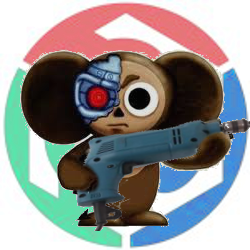
\includegraphics[height=0.4\textheight]{logo/CHBZ.png}
\hspace{1cm}

\includegraphics[height=0.15\textheight]{logo/LinuxPowered.png}
\hspace{1cm}

\includegraphics[height=0.4\textheight]{logo/OpenHardware.png}

\vspace{1.5cm}

\begin{centering}

{\Huge \textbf{\textsc{Азбука халтурщика-ARMатурщика \bigskip}}}

{\Huge \textbf{\textit{разработка встраиваемых систем}}}

{\Large 
основы бытовой автоматики,

систем управления и сбора данных
}

\end{centering}

\vspace{1cm}

{\large
\noindent
\copyright\
\href{https://groups.google.com/forum/\#!forum/openwrt2ru}{ruOpenWrt}
 \\
\copyright\
HackSpace
<<\href{https://github.com/ponyatov/CHBZ/raw/master/presentation.pdf}{Чебураторный
завод}>> \\
\copyright\
Консорциум хоббитов России
}
\end{titlepage}


\tableofcontents

% \clearpage\secly{О книге}

Эта книга\ --- комплект документации по аппаратно-программной платформе
ALYEH:

\begin{itemize}[nosep]
  \item \textcolor{red}{А}збука ARMатурщика
  \item \textcolor{red}{L}inux для встраиваемых систем
  \item д\textcolor{red}{Y}намический язык программирования \termdef{Ы}{Ы}
  \item библиотека \cpp\ для встраива\textcolor{red}{E}мых систем  
  \item \textcolor{red}{H}ardware библиотека универсальных модулей
\end{itemize}
\bigskip

\emph{В текущем состоянии эта книга\ --- конспект материалов, которые я сейчас
собираю, в черновой верстке. Объем материала очень большой, фактически это целая
специальность для приличного техникума, что-то типа ``Технология цифрового
производства''. Поэтому 146\% пока составляет сырая копипаста, с редкими
вкраплениями собственного бреда. В процессе адаптации, обкатки на студентах и
доработки эта поделка должна принять более вменяемый вид. Но учитывая полное
отсутствие обратной связи, этого никогда не случиться.}
\bigskip

Это учебное пособие было создано для интересующихся любительской электроникой,
самодельными цифровыми системами управления (Arduino, устройствами на
микроконтроллерах и т.п.), и программистов-лю\-би\-те\-лей. В связи с полной
деградацией системы образования пособие также рекомедуется для применения при
обучении в ВУЗах по специализациям, связанным с применением цифровой электроники
и компьютерной техники.

Большой упор был сделан на использование открытого некоммерческого программного
обеспечения, для удешевления учебного процесса, уменьшения себестоимости ваших
проектов\note{вряд ли ли у вас окажется лишняя пачка килобаксов на покупку пары
коммерческих САПР, по крайней мере пока ваш стартап не взлетит в Top\$100K}, и
стимулирования вашего участия в развитии этих программных пакетов.

Книга очень объемна и разнообразна по материалу, и построена как справочник с
группировкой материала по тематике. Для тех, кто только начинает, в разделе
\ref{learnplans}\ расписаны \termdef{пошаговые учебные планы}{учебный план} с
точки зрения параллельного изучения нескольких предметов с постепенным
усложнением\note{как это происходит при традиционном offline обучении}. Как
известно, главная часть любого обучения\ --- практическая. Особое внимание
уделено набору лабораторных работ.

\bigskip
В качестве видеоматериала были использованы 
\href{https://www.youtube.com/playlist?list=PLddc343N7YqgCWlspw08g6t0iFos9gAi4}{видеоуроки
физики}\\
\copyright\ Ерюткин Е.С., учитель физики высшей категории 
\href{http://sch1360v.mskobr.ru/}{ГБОУ СОШ №1360}, г.Москва

\bigskip
Мы признательны Bill Collis за разрешение использовать материалы его книги
<<\href{www.techideas.co.nz}{An Introduction to
Practical Electronics,
Microcontrollers and
Software Design}>> \cite{bcollis} в
русскоязычном варианте <<Азбуки>> (\ref{bcollis}), и конечно он вполне
заслуженно включен в основные соавторы этой книги.

\bigskip
Так как для работы в области электроники необходимо владение технологиями
изготовления конструктива, в книгу включен соответствующий раздел. 
Эти книги рекомендуются популярным поставщиком хоббийных настольных
микро-станков \href{http://sherline.com/}{Sherline Products}. Так как от
владельцев авторских прав не получено разрешение на полный официальный перевод,
для этих книг сделан только перевод-подстрочник, который поможет вам читать
оригинал:
\begin{itemize}
  \item Joe Martin, Craig Libuse \textbf{Tabletop Machining}
  \cite{tabletop} (\ref{tabletop})
  \item Doug Briney \textbf{Home Machinists Handbook}
  \cite{briney} (\ref{briney})
\end{itemize}

Отечественных книг по использованию маленьких ``часовых'' и настольных станков
просто не существует, хотя они и выпускались серийно. Исключение\ --- книга
Евгений Васильев \textbf{Маленькие станки} \cite{vasil}, но она имеет обзорный
характер.

\bigskip
\textbf{Лицензия на эту книгу пока не выбрана, так что она пока просто пишется в
духе OpenSource: любой может использовать ее часть, изменять или дополнять, до
тех пор, пока не накладываются какие-либо административные, финансовые или
юридические ограничения на распространение и развитие оригинальной версии или ее
открытых форков: \url{https://github.com/ponyatov/A}}
\bigskip

Приглашаем всех желающих участвовать в развитии этого учебного пособия на форум
\href{https://groups.google.com/forum/\#!forum/openwrt2ru}{ruOpenWrt} и в группу
\url{http://vk.com/samarahackerspace}, нам нужна обратная связь по качеству
материала, результаты тестирования на вас или ваших студентах, дополнения и
замечания.


% \secrel{Введение в практическую электронику} \label{bcollis}
% \addcontentsline{toc}{section}{An Introduction to 
Practical Electronics, 
Microcontrollers and
Software Design \copyright\ Bill Collis}

Эта часть основана на книге:
\bigskip

\textbf{An Introduction to 
Practical Electronics, 
Microcontrollers and
Software Design}

Second Edition, 01 May-2014

\copyright\ Bill Collis

\url{www.techideas.co.nz}

\bigskip
Мы признательны автору за разрешение использовать материалы его книги в
русскоязычном варианте <<Азбуки>>, и конечно он вполне заслуженно включен в
основные соавторы этой книги.

\bigskip
We are grateful to the author for permission to use materials of his book in the
russian version of <<Azbuka>>, and of course he was deservedly included in the
main co-authors of this book.

\bigskip
\begin{verbatim}
From: Bill Collis <Bill.Collis@..........nz>
Date: 2014-11-24 0:53 GMT+04:00
Subject: Electronis Book
To: "dponyatov@gmail.com" <dponyatov@gmail.com>

Hi Dmitry
thanks for your email.
I am looking at the future of the book myself and thinking I will open source
it. If you will only be in using it in Russian language then that is ok and you
need to reference the original book.

Thanks
Bill
\end{verbatim}

% \chapter{1 Введение в практическую электронику 13}

Эта книга\note{оригинал: B.Collis The Introduction to Practical 
Electronics\ldots}\ имеет слеующий ряд основных направлений:

\begin{itemize}
  \item Распознавание электронных компонентов и их правильное использование
  \item Наработка цельного набора компетенций в базовой электронике
  \item Использование макетных плат
  \item Навыки ручной пайки
  \item Использование закона Ома для выбора токоограничивающих резисторов
  \item Делитель напряжения
  \item Использование EDA CAD\note{\keys{E}\,lectronic \keys{D}\,esign
  \keys{A}\,utomation, САПР автоматизации проектирования электроники}\ для
  разработки и подготовки производства печатных плат
  \item Программирование микроконтроллеров и их сопряжение
  \item Транзистор в ключевом режиме
  \item Теория источников питания
  \item Принципы и схемы электропривода
  \item Моделирование решений через тестирование и испытания
  \item Следование кодексу практики
  \item Безопасные приемы работы
\end{itemize}

\section{Ваше обучение по специальности <<Технология>>}

\begin{itemize}

\item \textbf{Технологическая практика}

\begin{itemize}

\item\textbf{Быть четким}: разработка четких спецификаций для ваших
технологических проектов.

\item\textbf{Планирование}: думать прежде чем делать, и использовать во время
работы наброски типа блок-схем, принципиальных схем, чертежей разводки плат,
диаграмм и эскизов.

\item\textbf{Работа на результат}: испытания, тестирование и сборка электронных
схем, проектирование и изготовление печатных плат, написание программ для
микроконтроллеров.

\end{itemize}

\item \textbf{Технологические знания}

\begin{itemize}

\item\textbf{Технологическое моделирование}: прежде чем строить электронное
устройство, важно понять как оно работает сначала путем моделирования и/или
тестирования аппаратного и программного обеспечения.

\item\textbf{Технологические продукты}: знания о компонентах и ​​их
характеристиках.

\item\textbf{Технологические системы}: электронное устройство является более,
чем набором компонентов, это функционирующая система с входами, выходами и
контролирующим процессом.

\end{itemize}

\item \textbf{Nature of Technology}

\begin{itemize}

\item\textbf{Characteristics of Technological Outcomes} – knowing about
electronic components especially microcontrollers as the basis for modern technologies.

\item\textbf{Characteristics of Technology} – electronic devices now play a
central role in the infrastructure of our modern society; are we their masters, how have they changed our lives?

\end{itemize}

\end{itemize}

\section{Ключевые компетенции Ново-Зеландской программы}

\begin{itemize}

\item\textbf{Thinking} – to me the subject of technology is all about thinking.
My goal is to have students understand the technologies embedded within electronic devices. To achieve this students
must actively enage with their work at the earliest stage so that they can construct their own
understandings and go on to become good problem solvers. In the beginning of their learning
in electronics this requires students to make sense of the instructions they have been given
and search for clarity when they do not understand them. After that there are many new and
different pieces of knowledge introduced in class and students are given problem solving
exercises to help them think logically. The copying of someone elses answer is flawed but
working together is encouraged. At the core of learning isbuilding correct conceptual models
and to have things in the context of the ‘big picture’.

\item\textbf{Relating to others} – working together in pairs and groups is as
essential in the classroom as it is in any other situation in life; we all have to share and negotiate resources and equipment
with others; it is essential therefore to actively communicate with each other and assist one
other.

\item\textbf{Using language symbols and texts} – At the heart of our subject is
the language we use for communicating electronic circuits, concepts, algorithms and computer programming syntax; so
the ability to recognise and using symbols and diagrams correctly for the work we do is vital.

\item\textbf{Managing self} – This is about students taking personal
responsibility for their own learning; it is about challenging students who expect to read answers in a book or have a teacher tell them
what to do. It means that students need to engage with the material in front of them.
Sometimes the answers will come easily, sometimes they will not; often our subject involves a
lot of trial and error (mostly error). Students should know that it is in the tough times that the
most is learnt. And not to give up keep searching for understanding.

\item\textbf{Participating and contributing} – We live in a world that is
incredibly dependent upon technology especially electronics, students need to develop an awareness of the importance
of this area of human creativity to our daily lives and to recognise that our projects have a
social function as well as a technical one.

\end{itemize}

% 
\secrel{Вводная электронная схема}\label{bcentry}\secdown

\secrel{Где купить комплектующие?}

В Новой Зеландии есть некоторое количество отличных поставщиков компонентов с
разумными ценами, включающих \url{www.surplustronics.co.nz}, и
\url{www.activecomponents.com}. Зарубежные поставщики, которых я использую,
включают \url{www.digikey.co.nz}, \url{www.sparkfun.com}, \url{ebay.com}
и \url{aliexpress.com}.

\bigskip
Для России можно отметить сеть магазинов
``\href{http://voltmaster.ru/}{Больтмастер}''\note{\href{http://voltmaster-samara.ru/}{Самара}}.

\bigskip
Для модулей пока что доступна поставка из Китая по почте:
\href{http://www.aliexpress.com/}{AliExpress}\ с оплатой с виртуальной карты
VISA платежной системы \href{https://qiwi.ru/}{QIWI}. Доставка занимает от 2х
недель до 2х месяцев. Удобно покупать модули в виде микросхем, уже запаянных с
обвязкой на кусок текстолита (\term{breakout board}): Arduino Mini, Maple Mini,
датчики, контроллеры двигателей. Также интересны наборы (магазины) элементов:
пачки резисторов, конденсаторов и т.п. в выводном исполнении, по нескольку
десятков номиналов.

\secrel{Макетная плата: \term{breadboard}}

\begin{youtube}
\url{https://www.youtube.com/watch?v=vQdUSE1auz8}

\url{https://www.youtube.com/watch?v=k9jcHB9tWko}

\url{https://www.youtube.com/watch?v=2wvn8_23phE}

\end{youtube}

\bigskip
\noindent
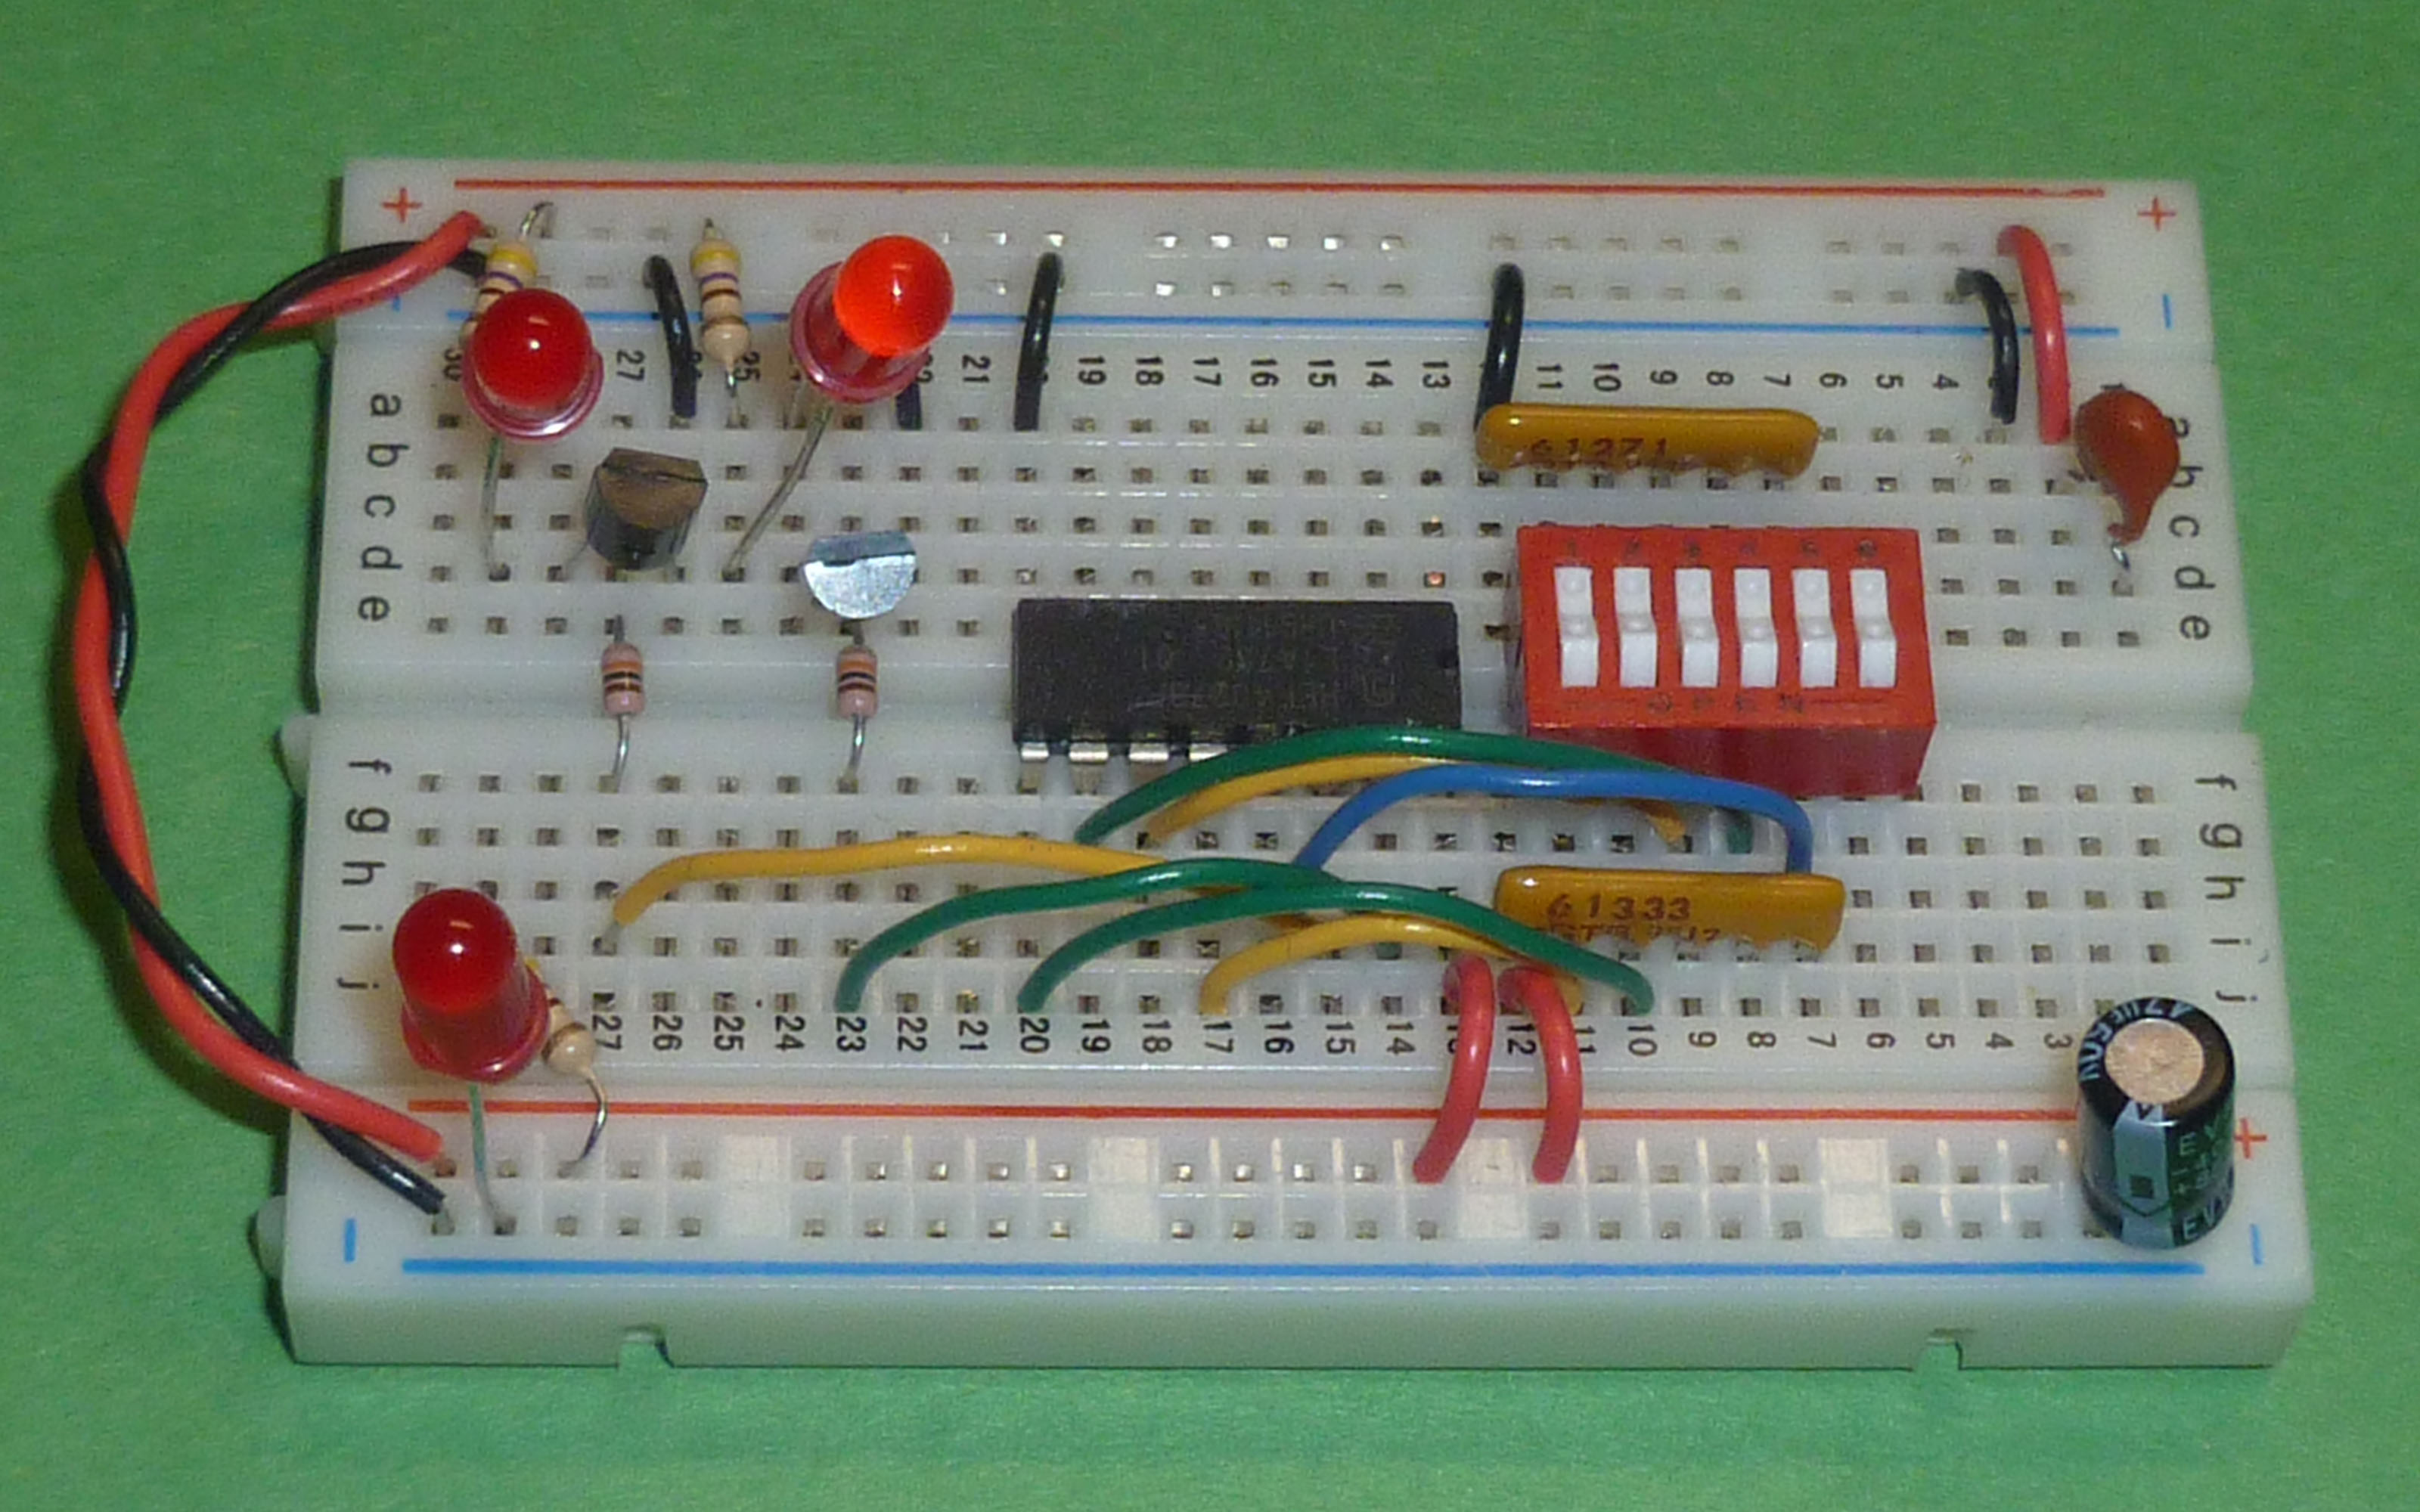
\includegraphics[height=0.3\textheight]{bcollis/breadboard2.jpg}
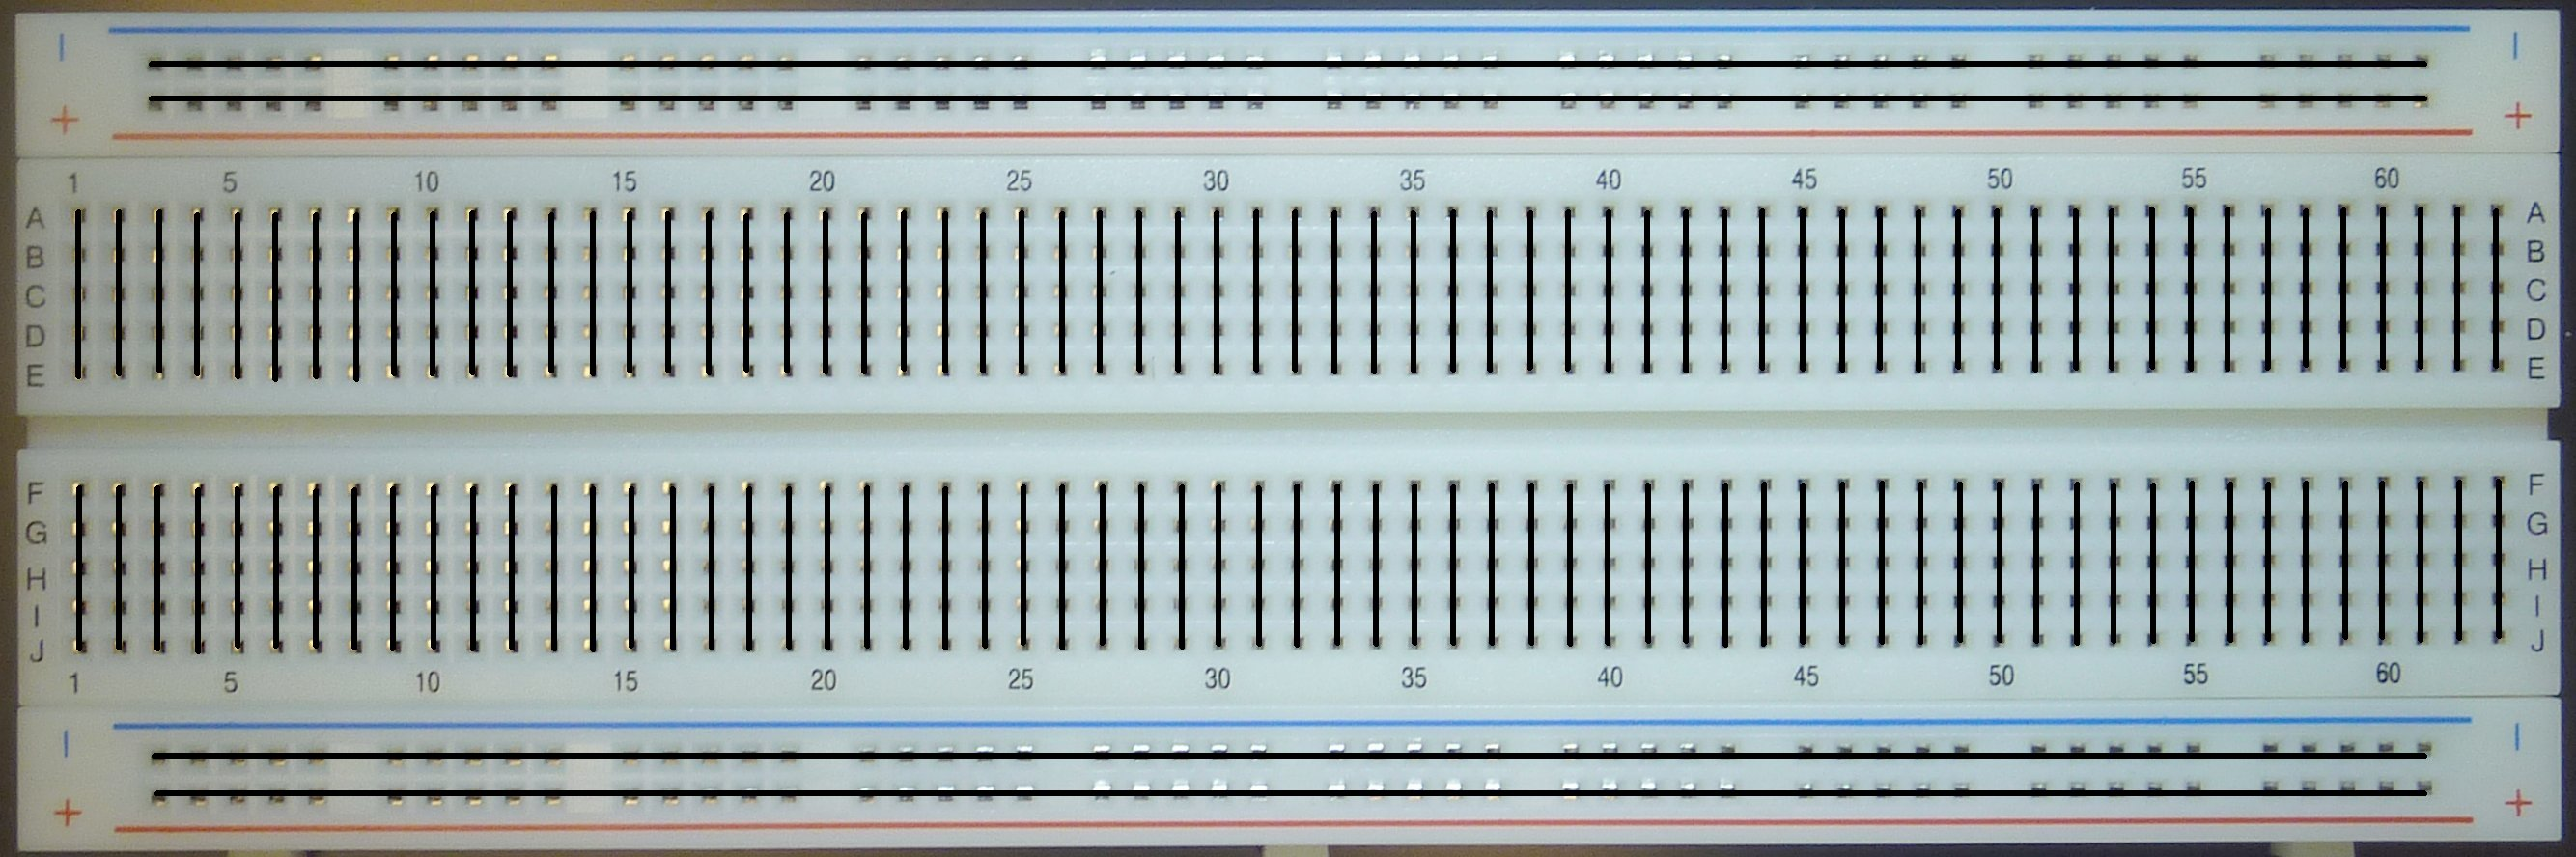
\includegraphics[height=0.3\textheight]{bcollis/BreadboardConnections.jpg}
\bigskip

\termdef{Breadboard}{breadboard} ([б]еспаечная \termdef{[м]акетная
[п]лата}{макетная плата} , \termdef{БМП}{БМП}, ``\termdef{вафля}{вафля}'')\ ---
пластмассовый блок с отверстиями и металлическими полоск\'{о}выми зажимами,
создающими соединения между \termdef{элементами схемы}{элемент}. Отверстия
расположены так, что \termdef{компоненты}{компонент} и отрезки провода могут
быть соединены вместе формируя схему, без использования паяльника. Верхние и
нижние ряды, как правило, используются для \termdef{шин питания}{шина питания},
красный сверху для плюса, и внизу черный/синий для минуса (\termdef{общий
провод}{общий провод}, или \termdef{``земля''}{земля}). На длинных вафлях шины
питания поделены на отдельные сегменты, и требуют соединения короткими
перемычками.

\secrel{Простейшая схема}

Эта схема может быть собрана вот так \ref{ch21lay}, обратите внимание, что
\termdef{светодиод}{светодиод} должен находиться в правильном положении. Если у
вас есть светодиод и \termdef{резистор}{резистор}, соединенные в
\termdef{замкнутый контур}{замкнутый контур}, светодиод должен загореться.

\bigskip
\noindent\begin{tabular}{p{0.45\textwidth} p{0.45\textwidth}}
Принципиальная схема \label{ch21sch}
&
Компоновка \label{ch21lay} \\
&\\
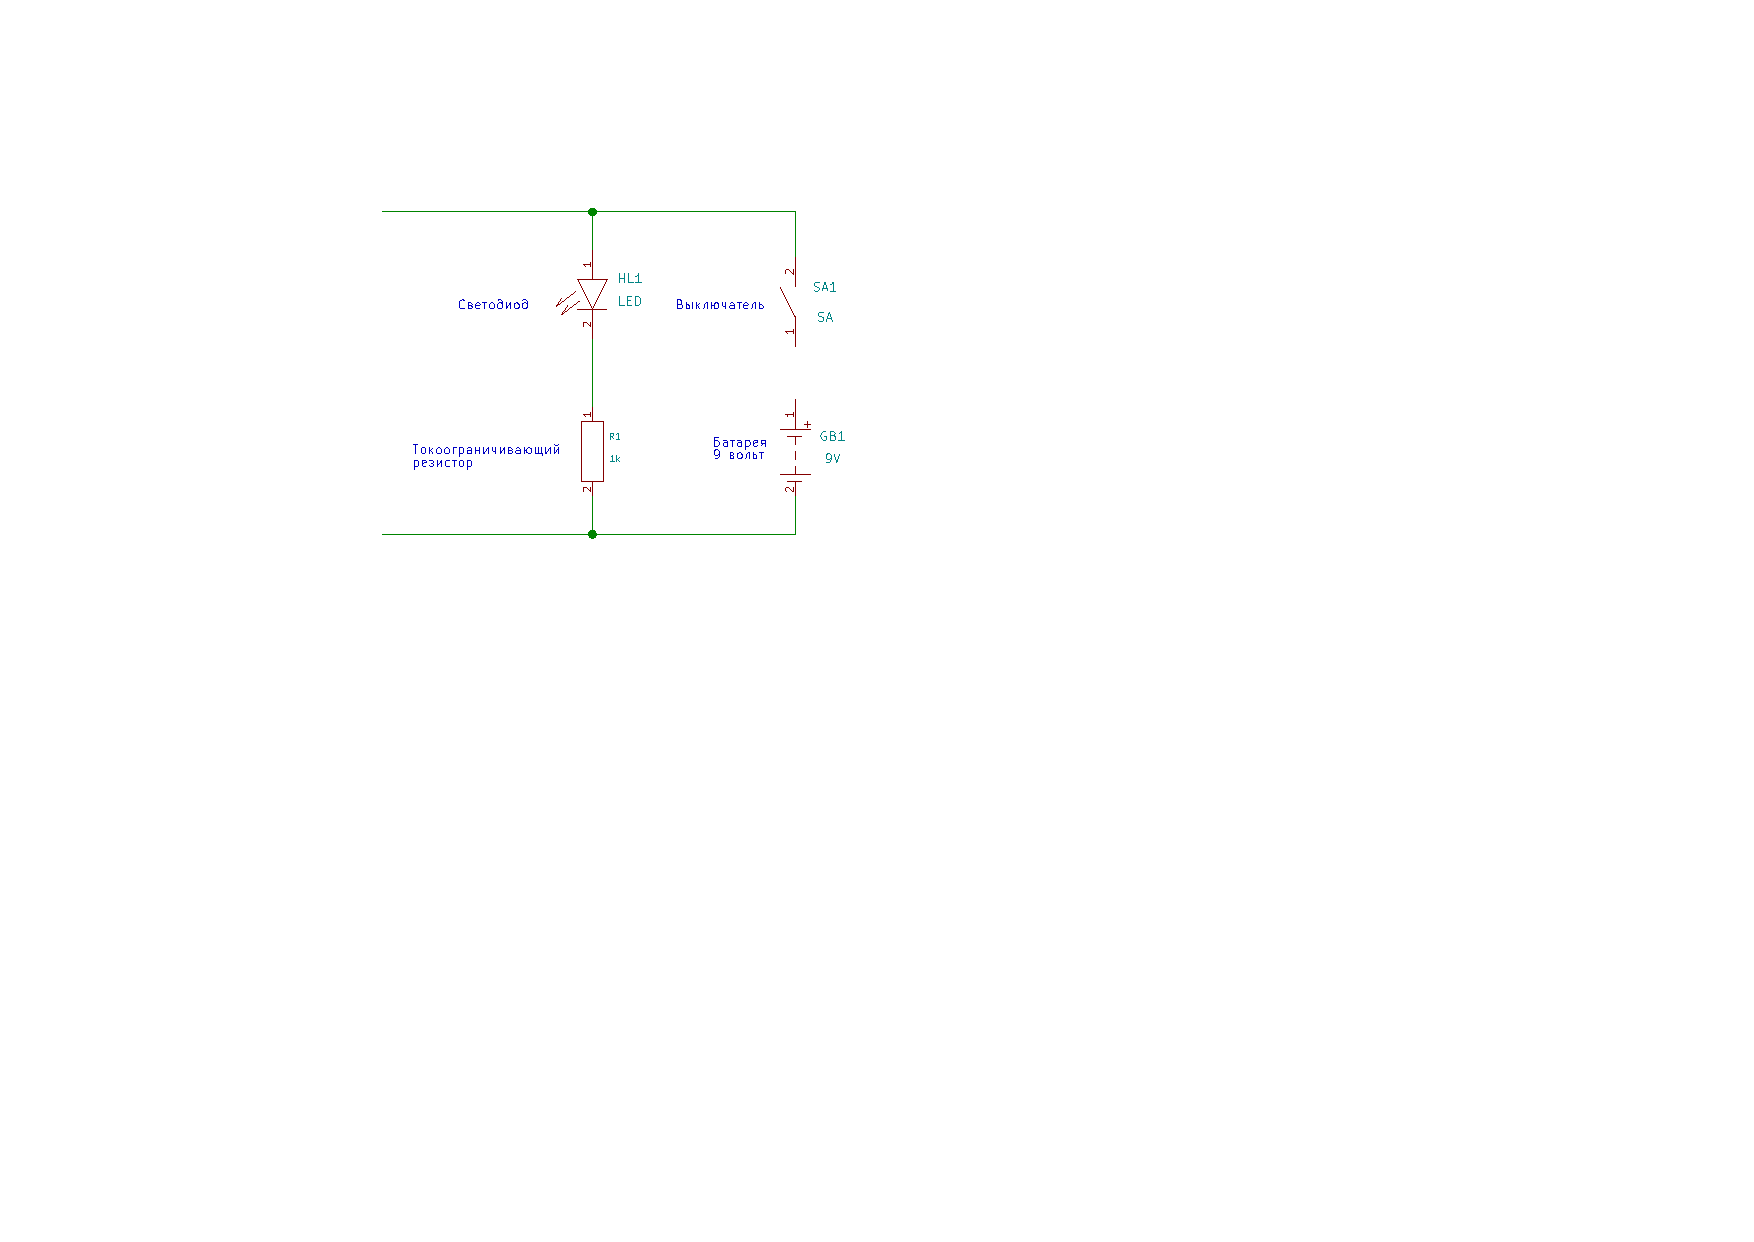
\includegraphics[width=0.45\textwidth]{bcollis/led1/led1.pdf}
&
\\
\end{tabular}

\bigskip
Светодиоду требуется \emph{для включения} около 2\,В\note{[В]ольт}, батарея на
9\,В, так что с напряжением все нормально. \emph{Но если вы подключите светодиод
напрямую к батарее, он сгорит! Для светодиодов главный рабочий параметр\ ---
\termdef{допустимый рабочий ток}{допустимый рабочий ток}, обычно он не превышает
10..20\,mA\note{1\,[м]иллиАмпер = 0.001\,[А]мпер}}. Так что
1\,k\note{1\,[К]илоОм = 1000\,Ом}\ резистор используется для ограничения тока
через светодиод.

\bigskip
Недопустимо подавать на светодиоды напряжение обратной полярности. Светодиоды
имеют невысокое (несколько вольт) обратное пробивное напряжение. В схемах, где
возможно появление обратного напряжения, светодиод должен быть защищён
параллельно включенным обычным диодом в противоположной полярности.

\bigskip
Если вы отключите любой провод в схеме, она перестает работать, схема должна
быть завершенной, чтобы электроны могли течь по проводникам из
\termdef{источника питания}{источник питания}.

\secrel{Ток и напряжение, сечение проводника, плотность тока}\label{bctok}

\begin{youtube}

\url{https://www.youtube.com/watch?v=Dq4fSp6wz-o}

\begin{enumerate}[nosep]
  \item \url{https://www.youtube.com/watch?v=3ZeveDL1\_bg}
  Электрический ток Источники тока
  \item \url{https://www.youtube.com/watch?v=mt86jYUjPFI}
  Ток в металлах Действия электрического тока 
  \item \url{https://www.youtube.com/watch?v=42CEi94hGgA}
  Электрический ток. Сила тока
  \item \url{https://www.youtube.com/watch?v=SNPO5e9wZWU}
  Амперметр Измерение силы тока
  \item \url{https://www.youtube.com/watch?v=Yt91alAwp68}
  Электрическое напряжение
\end{enumerate}

\end{youtube}

В предыдущем разделе были использованы два важных понятия электроники\ ---
\termdef{ток}{ток} и \termdef{напряжение}{напряжение}. Необходимо объяснить эти
понятия, не залезая глубоко в физику. Проще всего объяснить какое-то явление на
примере другого явления, с которым человек регуляроно сталкивается в обыденной
жизни, и ощущает его собственными органами чувств. Для электрических явлений
лучше всего подходит \termdef{гидравлическая модель}{гидравлическая
модель}\note{\href{http://edwpl.ucoz.ru/publ/fundamenty\_ehlektroniki/induktivnye_ehlementy/induktivnosti/5-1-0-18}{пример
применения} гидравлической модели, осторожно, г***осайт}.
В \termdef{ГМ}{ГМ} электрические явления заменяются условными водопроводными:
\termdef{проводник}{проводник}\ --- труба, \termdef{электрический
ток}{электрический ток}\ --- поток воды в этой трубе,
\termdef{резистор}{резистор}\ --- сужение сечения трубы, препятствующее течению
тока, \termdef{диод}{диод}\ --- клапан, открывающися только в одну сторону, и
т.п. В результате маловразумительные абстрактные понятия физики электрических
явлений превращаются в почти ощутимые потоки и давление воды: все мы ежедневно
пользуемся водопроводом, даже в глухих регионах найдется бочка или хотя
бы дырявое ведро.

\bigskip
Таким образом, любому школьнику можно объяснить эти понятия:

\begin{rulebox}
Электрическое \termdef{напряжение}{напряжение}\ --- давление ``электрической
воды'' в проводнике-трубе.\\
Измеряется в \termdef{[В]\'{о}льтах}{Вольт}. 
\end{rulebox}

Как и обычное давление, \emph{напряжение\ --- разностная величина, так как
измеряется между двумя точками} электрической цепи. Для обычного давления за
опорную величину принимают атмосферное давление\note{не ощущаемое человеком, так
как оно уравновешено таким же внутренним давлением крови}. Для электричества
напряжение измеряют тоже между двумя точками, или между точкой и \termdef{общим
проводом}{общий провод}, принимаемым за 0. В физике напряжение определяют также
как \termdef{разность потенциалов}{разность потенциалов} между двумя точками.

\begin{framed}\noindent
Если взять проводник, и разделить его условной плоскостью, перпендикулярной
проводнику, в области пересечения этой плоскости и проводника получается
область\ --- \termdef{сечение проводника}{сечение проводника}.
\end{framed}

Сечение проводника легко увидеть и реально\ --- достаточно взять
толстый одножильный сплошной провод, и аккуратно отпилить (не откусить) его
точно поперек. Поверхность такого отпила и будет сечением.

\begin{rulebox}
Электрический \termdef{ток}{ток}\ --- количество ``электрической
воды'', проходящей через сечение проводника-трубы в единицу времени.
\termdef{Сила тока}{сила тока} измеряется в \termdef{[А]мп\'{е}рах}{Ампер}.
\end{rulebox}

\begin{framed}\noindent
\begin{equation}
j = \frac{I}{S}
\end{equation}
\begin{tabular}{l l l}
где& $j$ & \termdef{плотность тока}{плотность тока}, $\mbox{А}/\mbox{м}^{2}$ \\
&$I$ & сила тока, Ампер \\
&$S$ & \termdef{площадь сечения проводника}{площадь сечения проводника},
$\mbox{м}^{2}$
\end{tabular}
\end{framed}

Чем выше плотность тока, тем больше нагревается проводник (подробнее см
\ref{joul}), поэтому она учитывается при выборе провода, и ширины приводников
печатных плат. В этом случае часто используется численно другая величина\ ---
$\mbox{А}/\mbox{мм}^{2}$.

\secrel{Проводники и изоляторы, сопротивление и проводимость}\label{bcohm}

\begin{youtube}
\begin{enumerate}[nosep]
  \item \url{https://www.youtube.com/watch?v=q4I1hZ5YQ2w}
Электрическое сопротивление проводника.    
  \item \url{https://www.youtube.com/watch?v=SlxOEEaQ4Cg}
Удельное сопротивление 
\end{enumerate}

\url{https://www.youtube.com/watch?v=FCkR-3YE5Ac}

\end{youtube}

Используя гидравлическую модель, точно так же просто можно объяснить понятие
\termdef{проводимости}{проводимость}. Любой материал можно представить как
кусок вещества, имеющий пористую структуру, например как поролон или песок.
Через этот пористый материал течет ``электрическая вода'', т.е. ток. Это течение
вызвано действием напряжения, \term{приложенного} к концам проводника
(источником питания). Напряжение проталкивает электричество через материал,
поэтому чем больше напряжение, тем выше сила проходящего тока. Каждый материал
имееет свою ``пористость'', чем она больше, тем больше \term{проводимость}:

\begin{framed}
\begin{equation}\label{igu}
I = G \ U
\end{equation}
\begin{tabular}{l l l}
где & $I$ & сила тока, А \\
& $G$ & проводимость, См (сименс) \\
& $U$ & напряжение, В \\ 
\end{tabular}
\end{framed}

Чаще вместо проводимости используют обратную величину\ ---
\termdef{сопротивление}{сопротивление}:

\begin{framed}
\begin{equation}
R = \frac{1}{G} = G^{-1}
\end{equation}
\begin{tabular}{l l l}
где & $G$ & проводимость, См (сименс)\\
& $R$ & сопротивление, Ом\\
\end{tabular}
\end{framed}

Соответственно, формула \ref{igu}\ превращается в описанный в любом школьном
учебнике физики \termdef{закон Ома для постоянного тока}{закон Ома!для
постоянного тока}:

\begin{rulebox}
\begin{equation}\label{ohmlaw}
I = \frac{R}{U}
\end{equation}
\end{rulebox}

В зависимости от проводимости или сопротивления материалы делят на несколько
видов:

\bigskip
\begin{tabular}{ l l l }
& $G$, проводимость & $R$, сопротивление \\
\hline
сверхпроводник & $\infty$ & 0 \\ 
\termdef{проводник}{проводник} & большая & низкое \\
\termdef{изолятор}{изолятор}, 
\termdef{диэлектрик}{диэлектрик} & низкая & высокое \\
\end{tabular}
\bigskip

В зависимости от внешних условий: температуры, давления, агрегатного состояния
вещества\note{плазма, газ, жидкость, твердое тело}, примесей\ --- одно и то же
вещество может быть как проводником, так и изолятором.

Типичные проводники: металлы, ионизированный газ (плазма), растворы солей в воде
(электролиты), \emph{влажное} дерево

Типичные диэлектрики: пластики, стекло, керамика, \emph{сухое} дерево, вакуум,
газы в т.ч. воздух.

\bigskip
В электронике очень часто нужно иметь в определенном месте схемы заданное
сопротивление, для этого выпускаются специальные элементы с \emph{точно
калиброванным сопротивлением} между \termdef{выводами}{вывод элемента}:
\termdef{резисторы}{резистор}, иногда применяют устаревшее название \termdef{сопротивление}{сопротивление}
(часто проволочное). Их делают из керамики, на которую наматывают проволоку, или
напыляют тонкую пленку из специальных металлических сплавов с высоким
сопротивлением\note{часто в состав входят никель, хром, вольфрам}.
Иногда используется только кусочек такого сплава без керамики.
Для качественной пайки выводы резисторов делают из хорошо проводящего металла,
хорошо смачиваемого расплавленным припоем.

\secrel{Диэлектрическая и тепловая прочность изоляции}\label{bcisol}

\bigskip
Для диэлектриков существует специальный параметр, характеризующий их способность
работать как изолятор\ --- \termdef{диэлектрическая прочность}{диэлектрическая
прочность}.

\begin{framed}\noindent
Чем выше диэлектрическая прочность, тем большее напряжение способен выдерживать
изолятор без разрушения.
\end{framed}

\begin{framed}\noindent
При повышении температуры диэлектрическая прочность уменьшается 
\end{framed}

Именно поэтому

\begin{alarmbox}
Запрещается использовать любые удлинители в свернутом состоянии, или
использовать электрический провод, свернутый бухтой (катушкой)
\end{alarmbox}

\begin{alarmbox}
Не допускается нагрев любых частей электронной схемы или элементов
конструкции выше 40..50$^{o}C$
\end{alarmbox}

Для любого диалектрика существует некоторое значение напряжения, при котором он
начинает пропускать ток. При прохождении тока материал нагревается (\ref{joul}).
В результате нагрева проходящим током или от соседних соприкасающихся
поверхностей у диэлектрика увеличивается проводимость, что приводит к еще
большему проходящему через него току, и дополнительному нагреву. 

Если тепло не отводится во внешнюю среду (например в середине катушки провода
смотанного удлинителя), температура продолжает повышаться. В некоторый момент
температура достигает значения, при котором слой изоляции размягчается,
утрачивает механическую прочность, и соседние проводники сближаются или
соприкасаются с плохим контактом (происходит \termdef{короткое
замыкание}{короткое замыкание}).

\alarm{В месте плохого контакта или большого тока температура резко повышается}
до значений, когда диалектрик воспламеняется или резко меняет химический состав,
распадаясь \emph{с выделением ядовитых соединений}\note{для типичной изоляции из
ПВХ\ --- сложные токсичные соединения с содержанием хлора} и полностью утрачивая
изолирующие свойства как в электрическом, так и в механическом смысле.

Самый опасный вариант, и типичный случай \termdef{выгорания проводки}{выгорание
проводки}\ --- \termdef{ток короткого замыкания}{ток короткого замыкания}
слишком маленький для срабатывания защитных устройств
(\termdef{предохранитель}{предохранитель}, \termdef{автомат}{автомат},
\termdef{устройство защитного отключения}{устройство защитного
отключения}, \termdef{УЗО}{УЗО}), но достаточный для нагрева изоляции до
температуры химического распада или воспламенения. Аварийного выключения не
происходит, а проводка продолжает гореть до победного конца. 

\secrel{Тепловое действие тока. Мощность}

\begin{youtube}
\begin{enumerate}[nosep]
  \item \url{https://www.youtube.com/watch?v=2LWAIOHRI8s}
  Нагревание проводников электрическим током \termdef{Закон Джоуля Ленца}{закон
  Джоуля Ленца}
  \item \url{https://www.youtube.com/watch?v=Mbt4OTgBRuw}
  \termdef{Мощность}{мощность} электрического тока
\end{enumerate}
\end{youtube}

\secrel{Масштабные множители}\label{bcmux}

\begin{youtube}
\url{https://www.youtube.com/watch?v=i3ABWmCl1EI} Перевод единиц измерения
\end{youtube}

Практически для всех единиц измерения необходимо использование
\termdef{масштабных множителей}{масштабные множители}, когда величины численно
или слишком большие (много цифр до запятой), или слишком маленькие (много цифр
после запятой):

\bigskip
\begin{tabular}{ l l l }
пико & p & $10^{-12}$ \\
nano & n & $10^{-9}$ \\ 
микро & u, $\mu$ & $10^{-6}$ \\ 
милли & m & $10^{-3}$ \\
\hline
кило & k, K & $10^{3}$ \\
мега & M & $10^{6}$ \\
гига & G & $10^{9}$ \\
\end{tabular}
\bigskip

10\,mA = $10 \times 10^{-3}$\ A = $10 \times 0.001$ A = 0.010 A

5\,КОм = $5 \times 10^{3}$ Ом = $5 \times 1000$ Ом = 5000 Ом

\secrel{Использование мультиметра}\label{bcmmetr}

\begin{youtube}
\url{https://www.youtube.com/watch?v=BEgvm4o-u2Q}

\url{https://www.youtube.com/watch?v=UMwYLwsPgCY}

\begin{enumerate}[nosep]
  \item \url{https://www.youtube.com/watch?v=GBuGSj1uPGk}
  \item \url{https://www.youtube.com/watch?v=VJ3RBS42IVY}
\end{enumerate}

\url{https://www.youtube.com/watch?v=q3R4s6WE1cI}
\end{youtube}

Возьмите мультиметр (\ref{mmetr}) и измерьте напряжение на резисторе, близко ли
оно к 7\,В ? Также измерьте ток через диод, не превышает ли он допустимый ?

\begin{framed}
\emph{Напряжение} измеряется \term{в [В]\'{о}льтах} подключением
\term{измерительного прибора} (мультиметра) \emph{параллельно}\ элементу, при этом нужно
\begin{itemize}
\item
\term{режим измерения} включить на
\term{режим измерения постоянного напряжение} $V-$/DCV (или переменного,
обозначается как $V\sim$/ACV) а
  \item \term{диапазон
измерения} \emph{выставить на максимальное значение напряжения}
\item
Последовательно уменьшая диапазон измерения, найдите диапазон, в котором
мультиметр показывает наибольшее количество знаков после запятой.
\end{itemize}
\end{framed}

Если диапазон
слишком большой, прибор покажет значение в районе 0, а если слишком низкий\ ---
выведет [1]. Обычно работают в диапазоне, соответствующем максимальому
напряжению питания (в нашем случае 20\,V\note{[V]olt = [В]ольт}), иногда для
слабых напряжений переключаясь на одну..две ступени ниже. Но\ ---
\emph{возможны случаи\note{в \emph{любых схемах} содержащих
\term{индуктивности}: катушки пр\'{о}вода, трансформаторы, электродвигатели,
динамики и т.п.} когда напряжение в части схемы на порядки (в десятки..тысячи
раз) превосходит напряжение питания}.

\begin{framed}
\emph{Ток} измеряется \term{в [А]мп\'{е}рах} подключением \term{измерительного
прибора} (мультиметра) \emph{последовательно}\ с элементом \term{в разрыв цепи}, при этом
нужно
\begin{itemize}
\item
\term{режим измерения} включить на
\term{режим измерения постоянного тока} $A-$/DCA (или переменного, обозначается
как $A\sim$/ACA) а
  \item \term{диапазон
измерения} \emph{выставить на максимальное значение тока}
\item
Последовательно уменьшая диапазон измерения, найдите диапазон, в котором
мультиметр показывает наибольшее количество знаков после запятой.
\end{itemize}
\end{framed}

Обратите внимание, что напряжение измеряется \term{вольтметром} на полностью
собранной схеме, а для измерения тока нужно изменять схему, включая в нее
\term{амперметр}. Если измерения тока нужно проводить на готовом устройстве,
иногда ставят 2хконтактный \term{джампер} (как на материнских платах
компьютеров): при измерении амперметр подключают к его контактам, а потом
джампер замыкают специальной съемной проводящей перемычкой. Этом прием вы можете
использовать в своих устройствах для регулярного измерения \term{тока
потребления}, и расчета \term{потребляемой мощности}:

\begin{equation}
W_{\mbox{потребляемая}}\mbox{[Ватт]} =
U_{\mbox{питания}}\mbox{[Вольт]}
\times
I_{\mbox{устройства/элемента}}\mbox{[Ампер]}
\end{equation}

\begin{framed}
Переключив мультиметр в \term{режим прозвонки (т\'{е}стера)}, можно проверить
\begin{itemize}
\item наличие
электрического соединения между двумя точками \emph{обязательно отключенной от
источника питания} схемы,
\item исправность диода или светодиода,
\item исправность конденсатора большой \term{емкости} и
\item любые другие случаи когда нужно определить что две точки электрически
соединены между собой, постоянно или временно.
\end{itemize}
\end{framed}

Если между \term{щщуп}ами мультиметра в режиме прозвонки\note{= тестера}\
\term{сопротивление} протекающему току не превышает 1\,КилоОм\note{см.
паспорт на прибор}, раздается звуковой сигнал.

Если щщупы подключить к исправному \emph{разряженному} конденсатору большой
емкости (``электролиту''), раздастся короткий целчок или даже ``пик''.

Тестером также можно определить тип и \term{цокол\'{е}вку\note{``раскопытку''}}
транзистора; как это сделать описано в \ref{vt}.

\emph{Диоды} проверяются двумя подключениями \emph{в разной полярности}\ --- при
\emph{красном щщупе} на \term{аноде (+)} диода (в \term{прямой полярности
включения}) диод проводит ток, а в \term{обратной полярности} нет (красный щщуп
на \term{катоде (-)}).

Проверьте \emph{светодиод}: отключите его из схемы, и проверьте как диод.
Если светодиод исправен, в \emph{прямой полярности} светодиод будет \emph{очень
слабо светиться}.

\secrel{Определение сопротивления резистора по цветовому коду}

Когда берете резистор, проверьте его \termdef{номинал}{номинал} (значение). В
наших схемах каждый резистор имеет свою цель, и значение выбирается в
зависимости от того, хотим ли мы б\'{о}льший или меньший ток в этой части цепи.
Чем выше \term{номинал} резистора, тем меньше ток. Чем ниже номинал резистора,
тем выше ток. Для \termdef{выводн\'{ы}х}{выводн\'{о}й корпус} резисторов,
которые мы будем использовать на макетках, маркировка наносится на корпус в
виде набора цветных полосок:

\bigskip
Цветовая маркировка на 5 цветных полосок:
\begin{tabular}{|l|l|l|l|l|}
\hline
 цифра & цифра & цифра & множитель & точность \\
\hline
\end{tabular}

\bigskip Цифра:
\begin{tabular}{l l l l l l l l l l}
0&1&2&3&4&5&6&7&8&9\\
\textcolor{Black}{$\blacksquare$} &
\textcolor{Brown}{$\blacksquare$} &
\textcolor{Red}{$\blacksquare$} &
\textcolor{Orange}{$\blacksquare$} &
\textcolor{Yellow}{$\blacksquare$} &
\textcolor{Green}{$\blacksquare$} &
\textcolor{Blue}{$\blacksquare$} &
\textcolor{Magenta}{$\blacksquare$} &
\textcolor{Grey}{$\blacksquare$} &
$\square$ \\
\end{tabular}

\bigskip Множитель:
\begin{tabular}{l l l l l l l l l l}
\textcolor{Black}{$\blacksquare$} & $10^{0}=1$ &
\textcolor{Brown}{$\blacksquare$} & $10^{1}=10$ &
\textcolor{Red}{$\blacksquare$} & $10^{2}=100$ &
\textcolor{Orange}{$\blacksquare$} & $10^{3}=1000$ \\
\textcolor{Yellow}{$\blacksquare$} & $10^{4}=10000$ &
\textcolor{Green}{$\blacksquare$} & $10^{5}=100000$ &
\textcolor{Blue}{$\blacksquare$} & $10^{6}=1000000$ \\
\textcolor{Gold}{$\blacksquare$} & $10^{-1}=0.1$ &
\textcolor{Silver}{$\blacksquare$} & $10^{-2}=0.01$ \\
\end{tabular}

\bigskip Точность:
\begin{tabular}{l l l l l l l l l l l}
\textcolor{Brown}{$\blacksquare$} & $\pm 1\%$ &
\textcolor{Red}{$\blacksquare$} & $\pm 2\%$ &
\textcolor{Gold}{$\blacksquare$} & $\pm 5\%$ &
\textcolor{Silver}{$\blacksquare$} & $\pm 10\%$ \\
\end{tabular}

\bigskip
\begin{tabular}{l l l l l l l l l l l l l}
-[&
\textcolor{Brown}{$\blacksquare$}&
\textcolor{Black}{$\blacksquare$}&
\textcolor{Black}{$\blacksquare$}&
\textcolor{Yellow}{$\blacksquare$}&
\textcolor{Brown}{$\blacksquare$}&
]- 
& $100\times 10^{4}\pm 1\%$ & 1M & 1 миллион Ом & 1M $\Omega$ & 1 000 000 Ом \\
&1&0&0&4&1\\
-[&
\textcolor{Brown}{$\blacksquare$}&
\textcolor{Black}{$\blacksquare$}&
\textcolor{Black}{$\blacksquare$}&
\textcolor{Red}{$\blacksquare$}&
\textcolor{Red}{$\blacksquare$}&
]- 
& $100\times 10^{2}\pm 2\%$ & 10k & 10 тысяч ом & 10,000 Ом & 10k $\Omega$ \\
&1&0&0&2&2\\
-[&
\textcolor{Brown}{$\blacksquare$}&
\textcolor{Black}{$\blacksquare$}&
\textcolor{Black}{$\blacksquare$}&
\textcolor{Brown}{$\blacksquare$}&
\textcolor{Gold}{$\blacksquare$}&
]- 
& $100\times 10^{1}\pm 5\%$ & 1k & 1 тысяча ом & 1000 Ом & 1k $\Omega$ \\
&1&0&0&1&5\\
-[&
\textcolor{Orange}{$\blacksquare$}&
$\square$&
$\blacksquare$&
\textcolor{Black}{$\blacksquare$}&
\textcolor{Brown}{$\blacksquare$}&
]- 
& $390\times 10^{0}\pm 1\%$ & 390R & 390 Ом & 390$\Omega$ \\
&3&9&0&0&1\\
-[&
\textcolor{Brown}{$\blacksquare$}&
\textcolor{Black}{$\blacksquare$}&
\textcolor{Black}{$\blacksquare$}&
\textcolor{Black}{$\blacksquare$}&
\textcolor{Brown}{$\blacksquare$}&
]- 
& $100\times 10^{0}\pm 1\%$ & 100R & 1000 Ом & 100$\Omega$ \\
&1&0&0&0&1\\
-[&
\textcolor{Yellow}{$\blacksquare$}&
\textcolor{Magenta}{$\blacksquare$}&
\textcolor{Black}{$\blacksquare$}&
\textcolor{Gold}{$\blacksquare$}&
\textcolor{Brown}{$\blacksquare$}&
]- 
& $470\times 10^{-1}\pm 1\%$ & 47R & 47 Ом & 47$\Omega$ \\
&4&7&0&-1&1\\
\end{tabular}

\secrel{Светодиоды}

\noindent
\begin{tabular}{p{0.7\textwidth}p{0.3\textwidth}}
\noindent\parbox[b]{0.65\textwidth}{В настоящее время светоизлучающие диоды
используются в индикаторах и дисплеях на различном оборудовании, однако они все
больше и больше используются в качестве замены для \termdef{галогенных
ламп}{лампа!галогенная} и \termdef{ламп
накаливания}{лампа!накаливания}\note{использующие светящиеся проводники внутри
стеклянных колб} во многих других приложениях. Они включают в себя ходовые огни
на транспорте, светофоры,  большие уличные TV-экраны.}&
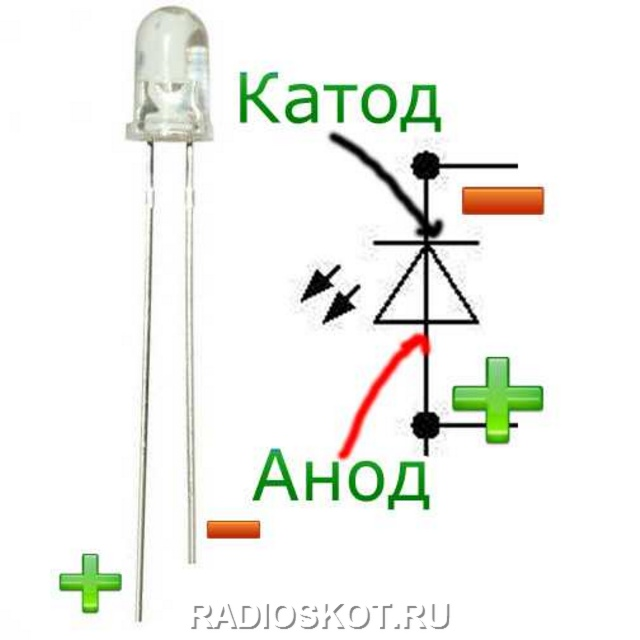
\includegraphics[width=0.25\textwidth]{bcollis/led.jpeg}
\\
\end{tabular}

\noindent
\begin{tabular}{p{0.3\textwidth} p{0.7\textwidth}}
\noindent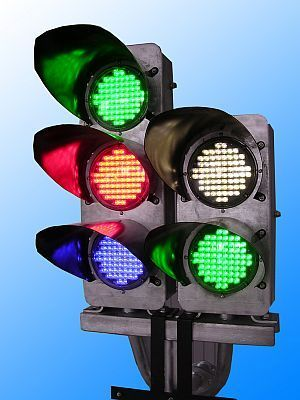
\includegraphics[width=0.3\textwidth]{bcollis/ledtraffic.jpeg}&
\noindent\parbox[b]{0.65\textwidth}{По сравнению с \term{лампами накаливания},
светодиоды почти не дают тепла, и поэтому очень эффективны. Они также имеют
гораздо б\'{о}льшее время жизни, например 10 лет, по сравнению с 10 месяцами для
ламп накаливания. Таким образом, в некоторых ситуациях например сигналов
светофора, если там установлены светодиоды, они дают значительную экономию как
по потребляемой мощности, так и по стоимости технического обслуживания. Хотя
есть небольшая проблема со светодиодными светофорами\ --- они не плавят снег,
который на них налипает!}\\
\end{tabular}

\secrel{Некоторые характеристики светодиодов}

\paragraph{\termdef{Интенсивность}{интенсивность}}: измеряется в мКд
(милликанделлах)

\paragraph{\termdef{Угол обзора}{угол обзора}}: угол от оси, до линии, где
интенсивность падает до 50\%

\paragraph{\termdef{Прямое напряжение}{прямое напряжение!светодиода}}:
напряжение необходимое для получения полной яркости светодиода

\paragraph{\termdef{Прямой ток}{прямой ток!светодиода}}: рабочий ток, дающий
максимальную яркость

\paragraph{\termdef{Пиковая длина волны}{пиковая длина волны}}: самая яркая
спектральная линия излучаемого света

\secrel{Задание на исследование светодиода}

Пользуясь сайтом одного из поставщиков, найдите информацию и
характеристики/атрибуты для двух светодиодов: обычный красный 5 мм и 5 мм
высокой интенсивности.


\bigskip
\begin{tabular}{|l|p{0.3\textwidth}|p{0.3\textwidth}|}

Cветодиод
&
Красный 5\,мм
&
Высокая интенсивность 5\,мм
\\
\hline

Поставщик&&\\

Номер детали&&\\

Стоимость (\$)&&\\

Яркость (мКд)&&\\

Прямое напряжение ($U_{F}$)&&\\

Длина волны (нм)&&\\

Прямой ток ($I_{F}$)&&\\

\end{tabular}

\clearpage\secrel{Добавление выключателя в схему}

Выключатель\ --- способ для ручного управления схемой пользователем

\bigskip\noindent
\begin{tabular}{p{0.45\textwidth} p{0.45\textwidth}}
Принципиальная схема
&
Компоновка
\\
\noindent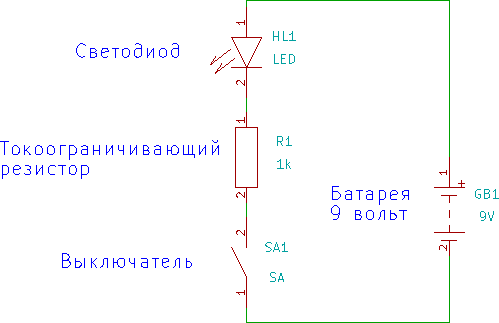
\includegraphics[width=0.45\textwidth]{bcollis/led2/led2.pdf}
&
\\
\end{tabular}

\secrel{2.7 Задание на установку выключателя 18}

2.7 Switch assignment

Find a small switch and carefully disassemble it (take it apart) draw how it
works and explain its operation. Make sure you explain the purpose of the
spring(s).

Here are simplified drawings of a small slide switch when it is in both
positions. When the switch is on electricity can flow, when it is open the
circuit is broken.


\secrel{Важные понятия схемотехники}

Кратко повторим:
\bigskip

Схема состоит из нескольких компонентов и источника питания, соединенных
проводами.

\emph{Поток электронов} (часто называют \termdef{носители заряда}{носители
заряда}) течет в цепи; однако если нет \emph{полной (замкнутой) цепи}, электроны
не могут течь.

\emph{Напряжение} (U) является мерой энергии в цепи, оно используется в качестве
меры энергии, подаваемой от батареи или энергии (напряжения) через часть схемы.

\emph{Ток (I) представляет собой поток электронов} от батареи по контуру и
обратно к батарее. Ток измеряется в амперах (обычно мы будем использовать
миллиампер или мА). Обратите внимание, что \emph{электрический ток это не ток
электронов или ток зарядов}. Так же, как течение реки не эквивалентно потоку
воды.

\emph{Сопротивление} работает \emph{на уменьшение тока}, резисторы в схеме
оказывают сопротивление току.

\emph{Проводники}, такие как провода, соединяющие компоненты вместе, не имеют
(теоретически) никакого сопротивления току.

\bigskip
Действительно важное понятие, для ясного понимания:

Напряжение прикладывается параллельно компонентам, а ток течет через компоненты.


% % \secrel{2.9 Изменение величины сопротивления 19}
% % \secrel{2.10 Добавление транзистора в схему 20}
% % \secrel{2.11 Чтение схем 21}
% % \secrel{2.12 Входная цепь\ --- LDR 22}
% % \secrel{2.13 Рабочая схема датчика темноты 23}
% % \secrel{2,14 Защитные цепи - использование диода 24}
% % \secrel{2.15 Задача исследования диода 24}
% % \secrel{2.13 Финальная схема датчика темноты 23}

\secup

% 
% \chapter{3 Вводное конструирование печатной платы 26}
% % 3.1 Eagle Schematic and Layout Editor Tutorial  26
% % 3.2 An Introduction to Eagle  27
% % 3.3 The Schematic Editor  28
% % 3.4 The Board Editor . 33
% % 3.5 Making Negative Printouts . 37
% % 3.6 PCB Making  38
% 
% \chapter{4 Пайка, припой и паяльники 41}
% % 4.1 Soldering facts . 42
% % 4.2 Soldering Safety  42
% % 4.3 Soldering wires to switches  43
% % 4.4 Codes of practice  44
% % 4.5 Good and bad solder joints  45
% % 4.6 Short circuits . 46
% % 4.7 Soldering wires to LED’s . 48
% \chapter{5 Введение в теорию электроники 49}
% % 5.1 Making electricity  49
% % 5.2 ESD electrostatic discharge  51
% % 5.3 Magnets, wires and motion  52
% % 5.4 Group Power Assignment  52
% % 5.5 Electricity supply in New Zealand  53
% % 5.6 Conductors  54
% % 5.7 Insulators  54
% % 5.8 Choosing the right wire  55
% % 5.9 Resistors . 56
% % 5.10 Resistor Assignment . 56
% % 5.11 Resistivity  56
% % 5.12 Resistor prefixes . 57
% % 5.13 Resistor Values Exercises . 58
% % 5.14 Capacitors  60
% % 5.15 Component symbols reference  61
% % 5.16 Year 10/11 - Typical test questions so far  62
% \chapter{6 Введение в электронику микроконтроллера 63}
% % 6.1 What is a computer? . 64
% % 6.2 What does a computer system do?  64
% % 6.3 What does a microcontroller system do? . 65
% % 6.4 What exactly is a microcontroller?  66
% % 6.5 Getting started with AVR Programming  67
% % 6.6 Breadboard  67
% % 6.7 Breadboard+Prototyping board circuit  68
% % 6.8 Checking your workmanship . 70
% % 6.9 Getting started with Bascom & AVR  71
% % 6.10 The compiler . 71
% % 6.11 The programmer . 71
% % 6.12 USBASP programming cable  72
% % 6.13 Your first circuit  73
% % 6.14 An introduction to flowcharts . 74
% % 6.15 Bascom output commands . 75
% % 6.16 Exercises  76
% % 6.17 Two delays . 77
% % 6.18 Syntax errors -‘bugs’ . 78
% % 6.19 Microcontroller portswrite a Knightrider program using LED’s  79
% % 6.20 Knightrider v2  80
% % 6.21 Knightrider v3  81
% % 6.22 Commenting your programs  83
% % 6.23 Learning review  83
% % 6.24 What is a piezo and how does it make sound?. 84
% % 6.25 Sounding Off . 85
% % 6.26 Sound exercises . 87
% % 6.27 Amp it up . 88
% \chapter{7 Входные цепи микроконтроллера 91}
% % 7.1 Single push button switch  91
% % 7.2 Pullup resistor theory  93
% % 7.3 Switch in a breadboard circuit  93
% % 7.4 Checking switches in your program  94
% % 7.5 Program Logic – the ‘If-Then’ Switch Test  95
% % 7.6 If-then exercises  96
% % 7.7 Switch contact bounce . 97
% % 7.8 Reading multiple switches  99
% % 7.9 Bascom debounce command . 100
% % 7.10 Different types of switches you can use  101
% % 7.11 Reflective opto switch  102
% \chapter{8 Обзор программирования 104}
% % 8.1 Three steps to help you write good programs  104
% % 8.2 Saving Programs . 104
% % 8.3 Organisation is everything  104
% % 8.4 Programming template  105
% % 8.5 What you do when learning to program . 106
% % 8.6 AVR microcontroller hardware  107
% % 8.7 Power supplies 107
% % 8.8 Programming words you need to be able to use correctly  110
% % 8.9 Year10/11 typical test questions so far  111
% \chapter{9 Введение в поток выполнения программы 112}
% % 9.1 Pedestrian crossing lights controller  112
% % 9.2 Pedestrian Crossing Lights schematic  113
% % 9.3 Pedestrian Crossing Lights PCB Layout 114
% % 9.4 Algorithm planning example – pedestrian crossing lights . 115
% % 9.5 Flowchart planning example – pedestrian crossing lights . 116
% % 9.6 Getting started code  117
% % 9.7 Modification exercise for the pedestrian crossing . 117
% % 9.8 Traffic lights program flow  118
% \chapter{10 Вводное программирование: использование подпрограмм 126}
% % 10.1 Sending Morse code  127
% % 10.2 LM386 audio amplifier PCB. 130
% % 10.3 LM386 PCB Layout . 132
% \chapter{11 Вводное программирование: Использование переменных 134}
% % 11.1 Stepping or counting using variables  135
% % 11.2 For-Next  137
% % 11.3 Siren sound - programming using variables  139
% % 11.4 Make a simple siren  141
% % 11.5 Siren exercise  142
% % 11.6 A note about layout of program code . 143
% % 11.7 Using variables for data  144
% % 11.8 Different types of variables  145
% % 11.9 Variables and their uses  146
% % 11.10 Vehicle counter  147
% % 11.11 Rules about variables  148
% % 11.12 Examples of variables in use . 148
% % 11.13 Byte variable limitations  149
% % 11.14 Random Numbers  150
% % 11.15 The Bascom-AVR simulator  151
% % 11.16 Electronic dice project  152
% % 11.17 Programming using variables – dice  152
% % 11.18 Dice layout stage 1 . 153
% % 11.19 Dice layout stage 2 . 154
% % 11.20 Dice Layout final 155
% % 11.21 First Dice Program flowchart . 156
% % 11.22 A note about the Bascom Rnd command  157
% % 11.23 Modified dice . 158
% % 11.24 Modified Knightrider  160
% \chapter{12 Основные дисплеи 161}
% % 12.1 7 segment displays . 161
% % 12.2 Alphanumeric LED displays  172
% \chapter{13 Проект портативного аудиоусилителя на TDA2822M 174}
% % 13.1 Portfolio Assessment Schedule . 175
% % 13.2 Initial One Page Brief . 176
% % 13.3 TDA2822M specifications  177
% % 13.4 Making a PCB for the TDA2822 Amp Project . 178
% % 13.5 Extra PCB making information  182
% % 13.6 Component Forming Codes of Practice. 183
% % 13.7 TDA2811 wiring diagram  184
% % 13.8 SKETCHUP Quick Start Tutorial  185
% % 13.9 Creating reusable components in SketchUp  186
% \chapter{14 Основы логического программирования 187}
% % 14.1 Quiz Game Controller  187
% % 14.2 Quiz game controller system context diagram  188
% % 14.3 Quiz game controller block diagram  188
% % 14.4 Quiz game controller Algorithm . 190
% % 14.5 Quiz game schematic . 191
% % 14.6 Quiz game board veroboard layout . 192
% % 14.7 Quiz Controller flowchart  196
% % 14.8 'Quiz Controller program code 197
% % 14.9 Don’t delay - use logic  199
% \chapter{15 Разработка алгоритма: Система сигнализации 202}
% % 15.1 Simple alarm system – stage 1 . 202
% % 15.2 Alarm System Schematic . 203
% % 15.3 A simple alarm system – stage 2 208
% % 15.4 A simple alarm system – stage 3 209
% % 15.5 A simple alarm system – stage 4 210
% % 15.6 More complex alarm system . 211
% % 15.7 Alarm unit algorithm 5 212
% % 15.8 Alarm 6 algorithm 213
% \chapter{16 Основы теории цепей постоянного тока 215}
% % 16.1 Conventional Current . 215
% % 16.2 Ground  215
% % 16.3 Preferred resistor values  215
% % 16.4 Resistor Tolerances  216
% % 16.5 Combining resistors in series . 216
% % 16.6 Combining resistors in parallel  217
% % 16.7 Resistor Combination Circuits  218
% % 16.8 Multimeters . 219
% % 16.9 Multimeter controls  220
% % 16.10 Choosing correct meter settings  221
% % 16.11 Ohms law  222
% % 16.12 Voltage & Current Measurements  223
% % 16.14 Continuity  224
% % 16.15 Variable Resistors  225
% % 16.16 Capacitors  226
% % 16.17 Capacitor Codes and Values . 226
% % 16.18 Converting Capacitor Values uF, nF , pF  226
% % 16.19 Capacitor action in DC circuits . 227
% % 16.20 The Voltage Divider  228
% % 16.21 Using semiconductors  229
% % 16.22 Calculating current limit resistors for an LED . 230
% % 16.23 The Bipolar Junction Transistor  231
% % 16.24 Transistor Specifications Assignment  232
% % 16.25 Transistor Case styles  232
% % 16.26 Transistor amplifier in a microcontroller circuit  232
% % 16.27 Transistor Audio Amplifier  233
% % 16.28 Speakers . 234
% % 16.29 Switch types and symbols  235
% \chapter{17 Основы планирования проекта 236}
% % 17.1 System Designer  237
% % 17.2 Project mind map . 241
% % 17.3 Project timeline . 243
% % 17.4 System context diagram  245
% % 17.5 Block Diagram 256
% % 17.6 Board Layouts  258
% % 17.7 Algorithm design  263
% % 17.8 Flowcharts  265
% \chapter{18 Пример дизайна системы: Таймер клеевого пистолета 268}
% % 18.1 System context diagram  268
% % 18.2 Hot glue gun timer block diagram . 269
% % 18.3 Hot glue gun timer algorithm . 270
% % 18.4 Hot glue gun timer flowchart  271
% % 18.5 Hot glue gun timer program. 272
% \chapter{19 Основные интерфейсы и их программирование 273}
% % 19.1 Parallel data communications  274
% % 19.2 LCDs (liquid crystal displays) . 275
% % 19.3 Alphanumeric LCDs  276
% % 19.4 ATTINY461 Development PCB with LCD . 277
% % 19.5 Completing the wiring for the LCD 279
% % 19.6 LCD Contrast Control  280
% % 19.7 Learning to use the LCD  281
% % 19.8 Repetition again - the ‘For-Next’ and the LCD  282
% % 19.9 LCD Exerises . 283
% % 19.10 Defining your own LCD characters . 286
% % 19.11 LCD custom character program  286
% % 19.12 A simple digital clock . 288
% % 19.13 Adding more interfaces to the ATTiny461 Development board . 290
% % 19.14 Ohms law in action – a multicoloured LED . 292
% \chapter{20 Основы интерфейса аналого-цифрового преобразования 295}
% % 20.1 ADC - Analog to Digital conversion . 295
% % 20.2 Light level sensing  295
% % 20.3 Voltage dividers review . 296
% % 20.4 AVR ADC connections  296
% % 20.5 Select-Case  297
% % 20.6 Reading an LDR’s values . 299
% % 20.7 Marcus’ year10 night light project . 301
% % 20.8 Temperature measurement using the LM35  304
% % 20.9 A simple temperature display . 305
% % 20.10 LM35 temperature display  309
% % 20.11 Force Sensitive Resistors  312
% % 20.12 Piezo sensor . 312
% % 20.13 Multiple switches and ADC . 313
% \chapter{21 Основы проектирования системы 314}
% % 21.1 Understanding how systems are put together  314
% % 21.2 Food Processor system block diagram . 314
% % 21.3 Subsystems  314
% % 21.4 Food Processor system functional attributes - algorithm  314
% % 21.5 Food Processor system flowchart  315
% % 21.6 Toaster Design 316
% % 21.7 Toaster - system block diagram  316
% % 21.8 Toaster Algortihm . 316
% \chapter{22 Основы проектирования системы: Тайм-трекер 317}
% % 22.1 System context diagram and brief  318
% % 22.2 Time tracker block diagram . 319
% % 22.3 Algorithm development . 320
% % 22.4 Schematic  320
% % 22.5 Time tracker flowchart and program version 1 321
% % 22.6 Time Tracker stage 2 . 322
% % 22.7 Time Tracker stage 3 . 324
% % 22.8 Time Tracker stage 4 . 326
% \chapter{23 Основы вычислений времени 330}
% % 23.1 Ohms law calculator  330
% % 23.2 more maths - multiplication . 335
% % 23.3 Algorithms for multiplication of very large numbers . 337
% % 23.4 Program ideas - algorithm and flowchart exercises . 339
% \chapter{24 Основы строковых переменных 340}
% % 24.1 Strings assignment . 342
% % 24.2 ASCII Assignment  344
% % 24.3 Time in a string . 347
% % 24.4 Date in a string  349
% % 24.5 Scrolling message assignment  351
% % 24.6 Some LCD programming exercises.  352
% \chapter{25 Cиловые интерфейсы 353}
% % 25.1 Microcontroller power limitations  353
% % 25.2 Power  355
% % 25.3 Power dissipation in resistors . 355
% % 25.4 Diode characteristics  356
% % 25.5 Using Zener diodes . 357
% % 25.6 How diodes work  358
% % 25.7 How does a LED give off light? . 359
% % 25.8 LCD Backlight Data . 360
% % 25.9 Transistors as power switches  361
% % 25.10 High power loads  362
% % 25.11 AVR Power matters  362
% % 25.12 Darlington transistors - high power . 364
% % 25.13 ULN2803 Octal Darlington Driver  366
% % 25.14 Connecting a FET backlight control to your microcontroller  368
% % 25.15 FET backlight control  369
% \chapter{26 Теория источников питания 370}
% % 26.1 Typical PSUs . 371
% % 26.2 The four stages of a PSU (power supply unit)  372
% % 26.3 Stage 1step down transformer  372
% % 26.4 Stage 2AC to DC Conversion  374
% % 26.5 Stage 3Filtering AC component . 375
% % 26.6 Stage 4Voltage Regulation  375
% % 26.7 Ripple (decibel & dB) . 379
% % 26.8 Line Regulation . 380
% % 26.9 Load Regulation  380
% % 26.10 Current Limit . 381
% % 26.11 Power, temperature and heatsinking . 384
% % 26.12 Typical PSU circuit designs  386
% % 26.13 PSU block diagram  386
% % 26.14 PSU Schematic  386
% % 26.15 Practical current limit circuit.  389
% % 26.16 Voltage measurement using a voltage divider  391
% % 26.17 Variable power supply voltmeter program  393
% \chapter{27 Типичные вопросы тестирования 2011/12/13 годов 395}
% \chapter{28 Расширенное программирование: Массивы 397}
% \chapter{29 Подтягивающие резисторы AVR 402}
% \chapter{30 Дополнительноподключение клавиатуры 403}
% % 30.1 Keypad program 1  403
% % 30.2 Keypad program 2  405
% % 30.3 Keypad program 3 – cursor control . 406
% % 30.4 Keypad texter program V1  409
% % 30.5 Keypad texter program 1a  413
% % 30.6 ADC keypad interface  414
% \chapter{31 Тонкости циклов Do-Loop \& While-Wend 417}
% % 31.1 While-Wend or Do-Loop-Until or For-Next? . 418
% \chapter{32 Подключение двигателя постоянного тока 423}
% % 32.1 H-мост 425
% % 32.2 H-Bridge Braking  427
% % 32.3 L293D H-Bridge IC  428
% % 32.4 L298 H-Bridge IC  430
% % 32.5 LMD18200 H-Bridge IC . 431
% % 32.6 LMD18200 program  434
% % 32.7 Darlington H-Bridge  435
% % 32.8 Stepper motors . 438
% % 32.9 PWM - pulse width modulation  445
% % 32.10 PWM outputs  446
% % 32.11 Uses for PWM  447
% % 32.12 ATMEL AVRs PWM pins . 448
% % 32.13 PWM on any port  449
% % 32.14 PWM internals  450
% \chapter{33 Пример расширенной системы: Будильник 452}
% % 33.2 Analogue seconds display on an LCD  457
% % 33.3 LCD big digits  460
% \chapter{34 Резистивный сенсорный экран 468}
% % 34.1 Keeping control so you dont lose your ‘stack’ . 474
% \chapter{35 Пример проектирования системы: Регулятор температуры 475}
% \chapter{36 Расширенное программирование: Машины состояний 478}
% % 36.1 Daily routine state machine . 478
% % 36.2 Truck driving state machine  480
% % 36.3 Developing a state machine  484
% % 36.4 A state machine for the temperature alarm system . 485
% % 36.5 Using System Designer software to design state machines  488
% % 36.6 State machine to program code  490
% % 36.7 The power of state machines over flowcharts  493
% % 36.8 Bike light – state machine example . 495
% % 36.9 Bike light program version1b  497
% % 36.10 Bike light program version2  499
% \chapter{37 Переработанный проект будильника 501}
% % 37.1 System Designer to develop a Product Brainstorm . 501
% % 37.2 Initial block diagram for the alarm clock  503
% % 37.3 A first (simple) algorithm is developed  505
% % 37.4 A statemachine for the first clock . 506
% % 37.5 Alarm clock state machine and code version 2 508
% % 37.6 Token game – state machine design example  509
% \chapter{38 Студенческий проект: Расширенный оконный контроллер 514}
% % 38.1 Window controller state machine #1  514
% % 38.2 Window controller state machine #3.  515
% % 38.3 Window controller state machine #5  516
% % 38.4 Window controller program . 517
% \chapter{39 Альтернативные техники кодирования машин состояния 524}
% \chapter{40 Сложно: последовательная связь 526}
% % 40.1 Simplex and duplex . 526
% % 40.2 Synchronous and asynchronous  526
% % 40.3 Serial communications, Bascom and the AVR  527
% % 40.4 RS232 serial communications  528
% % 40.5 Build your own RS232 buffer  530
% % 40.6 Talking to an AVR from Windows XP . 531
% % 40.7 Talking to an AVR from Win7 . 533
% % 40.8 First Bascom RS-232 program  535
% % 40.9 Receiving text from a PC . 536
% % 40.10 BASCOM serial commands  537
% % 40.11 Serial IO using Inkey()  538
% % 40.12 Creating your own software to communicate with the AVR  541
% % 40.13 Microsoft Visual Basic 2008 Express Edition . 542
% % 40.14 Stage 1 – GUI creation . 543
% % 40.15 Stage 2 – Coding and understanding event programming  552
% % 40.16 Microsoft Visual C# commport application  557
% % 40.17 Microcontroller with serial IO.  562
% % 40.18 PC software (C#) to communicate with the AVR . 567
% % 40.19 Using excel to capture serial data  571
% % 40.20 PLX-DAQ  573
% % 40.21 StampPlot  574
% % 40.22 Serial to parallel  576
% % 40.23 Keyboard interfacing – synchronous serial data  581
% % 40.24 Keyboard as asynchronous data . 588
% % 40.25 GPS  591
% \chapter{41 Цифровой радиоканал 597}
% % 41.1 An Introduction to data over radio  597
% % 41.2 HT12E Datasheet, transmission and timing  604
% % 41.3 HT12 test setup . 607
% % 41.4 HT12E Program  609
% % 41.5 HT12D datasheet . 610
% % 41.6 HT12D Program  612
% % 41.7 Replacing the HT12E encoding with software  613
% \chapter{42 Введение в I2C 617}
% % 42.1 I2C Real Time Clocks  618
% % 42.2 Real time clocks  619
% % 42.3 Connecting the RTC  619
% % 42.4 Connecting the RTC to the board . 619
% % 42.5 Internal features  620
% % 42.6 DS1307 RTC code  621
% % 42.7 DS1678 RTC code  626
% \chapter{43 Студенческий проект: Таймер полива теплицы 631}
% % 43.1 System block diagram  631
% % 43.2 State machine  631
% % 43.3 Program code  632
% \chapter{44 Проект Велосипедного аудиоусилителя 642}
% \chapter{45 Графические LCD 648}
% % 45.1 The T6963 controller  648
% % 45.2 Graphics LCD (128x64) – KS0108  653
% % 45.3 Generating a negative supply for a graphics LCD  658
% \chapter{46 Проект Отслеживания температуры GLCD 660}
% % 46.1 Project hardware  660
% % 46.2 Project software planning . 662
% % 46.3 Draw the graph scales  663
% % 46.4 Read the values  664
% % 46.5 Store the values  666
% % 46.6 Plot the values as a graph  667
% % 46.7 Full software listing . 669
% \chapter{47 Прерывания 672}
% % 47.1 Switch bounce problem investigation . 674
% % 47.2 Keypad- polling versus interrupt driven . 675
% % 47.3 Improving the HT12 radio system by using interrupts . 680
% % 47.4 Magnetic Card Reader  682
% % 47.5 Card reader data structure  682
% % 47.6 Card reader data timing  683
% % 47.7 Card reader data formats . 684
% % 47.8 Understanding interrupts in Bascom- trialling . 684
% % 47.9 Planning the program . 687
% % 47.10 Pin Change Interrupts PCINT0-31  690
% \chapter{48 Таймеры/Счётчики 692}
% % 48.1 Timer2 (16 bit) Program  693
% % 48.2 Timer0 (8bit) Program  694
% % 48.3 Accurate tones using a timer (Middle C) 695
% % 48.4 Timer1 Calculator Program . 696
% % 48.5 Timer code to make a siren by varying the preload value . 697
% \chapter{49 Проект скроллинга графического LED дисплея: массивы и таймеры 698}
% % 49.1 Scrolling text code  701
% % 49.2 Scrolling text – algorithm design  703
% % 49.3 Scrolling test - code  704
% \chapter{50 Проект медицинского прибора: реализация таймера 709}
% % 50.1 Block diagram  709
% % 50.2 Blower - state machine  710
% % 50.3 Blower program code . 711
% \chapter{Проект часов на 7-сегментном индикаторе\\
% реализация на сдвоенном таймере}
% % 51.1 Understanding the complexities of the situation  715
% % 51.2 Hardware understanding. 716
% % 51.3 Classroom clock – block diagram . 717
% % 51.4 Classroom clock - schematic  718
% % 51.5 Classroom clock - PCB layout  718
% % 51.6 Relay Circuit Example  719
% % 51.7 Classroom clock – flowcharts . 723
% % 51.8 Classroom clock – program . 724
% \chapter{52 ИС драйвера дисплея MAX 7219/7221 739}
% % 52.1 AVR clock/oscillator  743
% \chapter{53 Подключение через мобильную связь: ADH8066 744}
% % 53.1 ADH prototype development  745
% % 53.2 ADH initial test setup block diagram  747
% % 53.3 Process for using the ADH  748
% % 53.4 ADH communications . 750
% % 53.5 Initial state machine  751
% % 53.6 Status flags . 752
% % 53.7 Second state machine  753
% % 53.8 StateMachine 3 . 754
% % 53.9 Sending an SMS text . 755
% % 53.10 Receiving an SMS text . 756
% % 53.11 Splitting a large string (SMS message)  757
% % 53.12 Converting strings to numbers  760
% % 53.13 Full Program listing for SM3  761
% \chapter{54 Передача данных через \internet\ 778}
% % 54.1 IP address  779
% % 54.2 MAC (physical) address  779
% % 54.3 Subnet mask  780
% % 54.4 Ping  780
% % 54.5 Ports  781
% % 54.6 Packets . 781
% % 54.7 Gateway 782
% % 54.8 DNS  784
% % 54.9 WIZNET812  785
% % 54.10 Wiznet 812 Webserver V1  792
% % 54.11 Transmitting data  797
% % 54.12 Wiznet Server2 (version1)  809
% % 54.13 ‘Main do loop . 811
% % 54.14 process any messages received from browser . 812
% % 54.15 Served webpage . 814
% \chapter{55 Задание: математика в реальном мире 816}
% % 55.1 Math sssignment - part 1  819
% % 55.2 Math assignment - part 2 . 820
% % 55.3 Math assignment - part 3 . 821
% % 55.4 Math assignment - part 4 . 822
% % 55.5 Math assignment - part 5 . 823
% % 55.6 Math assignment - part 6 . 824
% % 55.7 Extension exercise  824
% \chapter{56 Цветной графический LCD на основе SSD1928 825}
% % 56.1 System block diagram  825
% % 56.2 TFT LCDs  826
% % 56.3 System memory requirements  827
% % 56.4 System speed  827
% % 56.5 SSD and HX ICs  827
% % 56.6 Colour capability  827
% % 56.7 SSD1928 and HX8238 control requirements  828
% % 56.8 SSD1928 Software . 829
% % 56.9 SSD1928 microcontroller hardware interface . 833
% % 56.10 Accessing SSD control registers . 834
% % 56.11 SSD1928_Register_routines.bas  836
% % 56.12 Accessing the HX8238.  840
% % 56.13 SSD1928_GPIO_routines.bas  840
% % 56.14 LCD timing signals . 842
% % 56.15 HX setups  843
% % 56.16 SSD setups  844
% % 56.17 SSD line / HSync timing  845
% % 56.18 SSD row / VSync/ frame timing  846
% % 56.19 HX and SSD setup routine . 848
% % 56.20 'SSD1928_HardwareSetup_Routines.bas  848
% % 56.21 SSD1928_Window_Control_Routines.bas . 852
% % 56.22 Colour data in the SSD memory  855
% % 56.23 Accessing the SSD1928 colour memory . 856
% % 56.24 'SSD1928_Memory_Routines.bas  856
% % 56.25 Drawing simple graphics . 858
% % 56.26 'SSD1928_Simple_Graphics_Routines.bas  858
% % 56.27 SSD1928_text_routines  861
% \chapter{57 Светофор: помощь и решение 865}
% \chapter{58 Компьютерное программирование: низкоуровневые детали 869}
% % 58.1 Low level languages869
% % 58.2 AVR Internals – how the microcontroller works . 870
% % 58.3 1. The 8bit data bus  871
% % 58.4 2. Memory  871
% % 58.5 3. Special Function registers  872
% % 58.6 A simple program to demonstrate the AVR in operation  872
% % 58.7 Bascom keyword reference . 874
% \chapter{59 USB-программатор: USBASP 876}
% \chapter{60 Программатор USBTinyISP 877}
% \chapter{61 Программирование на Си и AVR 881}
% % 61.1 Configuring a programmer  882
% % 61.2 First program . 884
% % 61.3 Output window  886
% % 61.4 Configuring inputs & outputs  887
% % 61.5 Making a single pin an input  888
% % 61.6 Making a single pin an output . 889
% % 61.7 Microcontroller type . 890
% % 61.8 Includes  890
% % 61.9 Main function . 891
% % 61.10 The blinkyelled program  892
% % 61.11 Counting your bytes  893
% % 61.12 Optimising your code  895
% % 61.13 Reading input switches  896
% % 61.14 Macros . 897
% % 61.15 Auto-generated config from System Designer  898
% % 61.16 Writing your own functions . 900
% % 61.17 AVR Studio editor features . 902
% % 61.18 AVR hardware registers  903
% % 61.19 Character LCD programming in C  904
% % 61.20 CharLCD.h Header file . 904
% % 61.21 Manipulating AVR register addresses  907
% % 61.22 Writing to the LCD  908
% % 61.23 Initialise the LCD . 910
% % 61.24 lcd commands  912
% % 61.25 Writing text to the LCD . 913
% % 61.26 Program Flash and Strings . 915
% % 61.27 LCD test program1 . 917
% % 61.28 CharLCD.h . 919
% % 61.29 CharLCD.c . 922
% \chapter{62 Объектно-Ориентированное Программирование (ООП) на \cpp\ и AVR 929}
% % 62.1 The black box concept  929
% % 62.2 The concept of a class  929
% % 62.3 First CPP program  930
% % 62.4 Creating an AVR CPP program in Atmel Studio 6  932
% % 62.5 Adding our class files to the project . 936
% % 62.6 First Input and output program  938
% % 62.7 Class OutputPin  940
% % 62.8 Class InputPin  940
% % 62.9 Inheritance  942
% % 62.10 Class IOPin  942
% % 62.11 Encapsulation  944
% % 62.12 Access within a class  944
% % 62.13 Class Char_LCD . 945
% % 62.14 Exercise – create your own Led class. . 950
% \chapter{63 Современные (2014) отладочные платы на AVR 953}
% % 63.1 Year10 ATTiny461 V4a development board  953
% % 63.2 Year11 ATTiny461 V7a development board  956
% % 63.3 Year 12 ATMega 20x4 Character LCD v6A . 959
% % 63.4 Year 13 ATMega GLCD 128x64 (2014) Veroboard . 961
% % 63.5 Year 13 ATMega GLCD (older pin connections)  966
% % 63.6 ATMEGA microcontroller pin connections  968
% % 63.7 ATMEGA16/644 40pin DIP package– pin connections . 969
% \chapter{64 Eagle: создание собственной библиотеки 970}
% % 64.1 Autorouting PCBS  977
% \chapter{65 Практические методы 979}
% % 65.1 PCB Mounting  979
% % 65.2 Countersink holes and joining MDF/wood  980
% % 65.3 MDF  981
% % 65.4 Plywood  981
% % 65.5 Acrylic  982
% % 65.6 Electrogalv  982
% % 65.7 Choosing fasteners . 983
% % 65.8 Workshop Machinery . 984
% % 65.9 Glues/Adhesives  986
% % 65.10 Wood Joining techniques  987
% % 65.11 Codes of Practice for student projects  988
% % 65.12 Fitness for purpose definitions and NZ legislation  989
% \chapter{66 ЧПУ 990}
% % 66.1 Machine overview  991
% % 66.2 Starting the CNC machine  992
% % 66.3 CamBam  993
% % 66.4 CamBam options . 993
% % 66.5 Drawing shapes in CamBam  994
% % 66.6 Machining commands  996
% % 66.7 A Box of Pi  997
% % 66.8 Holding Tabs  1003
% % 66.9 Engraving  1004
% % 66.10 Polylines  1005
% \chapter{67 Индекс 1008}


% % \chapter{KiCAD}

\cp{http://teholabs.com/knowledge/kicad.html}

\noindent
\includegraphics[height=0.5\textheight]{tmp/icon_kicad.png}


\cp{http://ru.wikibooks.org/wiki/KiCad}

KiCad\ --- распространяемый по лицензии GNU GPL программный комплекс САПР EDA с
открытыми исходными текстами, предназначенный для разработки электрических схем
и печатных плат.

Кроссплатформенность компонентов KiCad обеспечивается использованием 
библиотеки wxWidgets. Поддерживаются операционные системы Linux, 
Windows NT 5.x, Free\-BSD и Solaris.

Разработчик\ --- Жан-Пьер Шарра (фр. Jean-Pierre Charras), исследователь 
в LIS (фр. Laboratoire des Images et des Signaux\ --- Лаборатория Изображений 
и Сигналов) и преподаватель электроники и обработки изображений в фр. 
IUT de Saint Martin d’Hères (Франция).

\cp{http://ru.wikibooks.org/wiki/KiCad/Miniurok}

Этот раздел познакомит Вас с основами использования системы KiCad. Он содержит
информацию о всех шагах создания простой печатной платы: от рисования
электрической схемы до печати готового рисунка платы. Вам будут представлены
различные возможности KiCad и предложены эффективные пути решения различных
задач.

Руководство пользователя, поставляемое вместе с KiCad, содержит значительно
больше информации, чем этот урок. Ознакомтесь с ним, чтобы узнать больше об
использовании программы.



\secrel{Установка}\secdown

\secrel{\win}\label{kicadinstwin}

\menu{\winr{\url{http://www.kicad-pcb.org/}}>Download>\winstart}

\menu{\winr{\url{http://kicad.nosoftware.cz/}}>
\file{KiCad\_testing\-201x.xx.xx-BZRxxxx\_Win\_full\_version.exe}}

\bigskip

\menu{Installer Language>\emph{English}>Ok} 
в русифицированном инсталляторе кривые шрифты

\menu{KiCAD 20xx.xx.xx Setup>Next}

\menu{Лицензия>Agree}

\menu{Components>\checkbox\ все>Next}

\menu{Location>\file{C:/KiCad}>Install}

\menu{Completing Setup>\uncheckbox Wings3D>Finish}

\secrel{\linux}\label{kicadinstlin}

\begin{verbatim}
root# aptitude install kicad-doc-ru kicad
\end{verbatim}

\lst{+++\ $\sim$/.blackbox/menu}{}{/tmp/kicad.bbmenu}

\secrel{Настройка библиотек}

Для добавления библиотек, поставляемых с этой книгой, сделайте \emph{git
clone} или \emph{git pull}:

\begin{verbatim}
user:~$ git clone --depth=1 -o gh https://github.com/ponyatov/odurino.git odurino
user:~$ cd odurino
user:~/odurino$ git pull
\end{verbatim}

\menu{\prog{kicad}>\prog{eeschema}>Настройки>Библиотека}

\menu{Пользовательские пути поиска>Добавить>\file{/home/user/odurino/lib}}

\menu{Файлы библиотек>все стандартные>Удалить>OK}

\menu{Файлы библиотек>Добавить>R,L,C,SPICE,DA\_POWER,..>Открыть>OK}

\bigskip
Для проверки работы библиотек можете открыть проект

\menu{\prog{kicad}>Файл>Открыть>\file{~/Azbuka/bcollis/led1/led1.pro}}

или сразу схему

\menu{\prog{eeschema}>Файл>Открыть>\file{~/Azbuka/bcollis/led1/led1.sch}}

\secrel{Дотфайлы}

Посколько программа изначально писалась как юниксовая, пользовательские
настройки хранятся в dot-файлах:

\lst{~/.kicad}{}{kicad/kicad.dotfile}

\begin{description}
\item[KicadFrame*] размеры и положение окна менеджера проектов
\item[WorkingDir] каталог с текущим рабочим проектом
\item[fileN] список последних проектов (\ \menu{Файл>Последние файлы}\ )
\end{description}

\lst{~/.eeschema}{}{kicad/eeschema.dotfile}

\begin{description}
\item[SchematicFrame*] размеры и положение окна \prog{eeschema}
\item[fileN] список последних схем (\ \menu{Файл>Последние файлы}\ )
\end{description}

\secrel{Глобальные шаблоны}\label{kicadtemplates}

После установки \kicad\ можно скорректировать файлы глобальных шаблонов, чтобы
новые проекты создавались сразу с нужными настройками, прежде всего с нужным
нам набором библиотек:

\begin{verbatim}
sudo vim /usr/share/kicad/template/kicad.pro
\end{verbatim}

\lst{/usr/share/kicad/template/kicad.pro}{}{kicad/kicad.template}

\begin{description}
\item[LibDir] каталог библиотек, установите на свой или корпоративный/групповой
\item[LibNameN] задается список библиотек по умолчанию, приопишите ваш типовой
набор
\item[eeschema/libraries] схемные библиотеки \eeschema
\item[pcbnew/libraries] библиотеки надстеков для печатных плат \pcbnew
\end{description}

\secup


\section{Создание проекта в менеджере проектов \prog{kicad}}

В верхней части панели \term{менеджера проектов} \prog{kicad}
имеются большие кнопки запуска компонентов KiCad:

\begin{itemize}
\item \icoesch\ \prog{EeSchema}\ --- Редактор принципиальных схем
\item
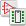
\includegraphics[height=0.1\textheight]{tmp/icon_cvpcb.png}\
\prog{CvPcb}\
--- Программа редактирования падстеков (отверстий и площадок)
\item 

\includegraphics[height=0.1\textheight]{tmp/icon_pcbnew.png}
\prog{Pcbnew}\ ---
Редактор печатных плат
\item

\includegraphics[height=0.1\textheight]{tmp/icon_gerbview.png}
\prog{GerbView}\ --- Программа просмотра фотошаблонов в формате Gerber
\item \prog{Bitmap2Component}\ --- Создание компонента из черно-белого
изображения (например логотипа)
\item 
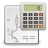
\includegraphics[height=0.1\textheight]{tmp/icon_pcbcalculator.png}
\prog{PcbCalculator}\ --- Калькулятор для печатных плат
\item 
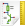
\includegraphics[height=0.1\textheight]{tmp/icon_pagelayout.png}
\prog{PageLayout}\ --- редактор формата листа схемы
\end{itemize}

Каждая кнопка запускает соответствующую программу. Мы будем использовать эти
программы по мере изучения.

\bigskip
Лучше всего для каждого проекта использовать раздельные папки; в противном
случае система может сбиться с толку, если файлы из разных проектов будут лежать
в одной папке. Проделайте следующие шаги:

\begin{enumerate}
  \item Создайте папку проекта \file{D:/ARM/SpindleDriver}
  \item Запустите программу KiCad
  \item Создайте проект (project)
  \begin{itemize}
    \item 
На панели инструментов KiCad выберите левую иконку с подсказкой\\
\menu{Начать новый проект}, используйте команду меню
\menu{Файл>Новый>Пустой} или сочетание клавиш \keys{Ctrl+N}.
    \item 
В диалоге \menu{Создать новый проект} выберите созданную папку
выберите только что созданную папку \file{D:/ARM/SpindleDriver} и
введите имя проекта \menu{\file{SpindleDriver}} и нажмите \menu{Сохранить}.
	\item
Если папка проекта содержит какие-то файлы, будет выведено окно выбора:
создать подпапку с именем проекта \menu{Yes}, или записать файл проекта
в указанную папку как есть \menu{No}. Нажмите No.
    \item 
Сохраните проект кнопкой \menu{Сохранить текущий проект}, \menu{Файл>Сохранить}
или \keys{Ctrl+S}.
	\item
В папке появится файл \file{SpindleDriver.pro}, содержащий установки вашего 
проекта. Файл имеет тектовый формат, поэтому при необходимости его можно открыть
в любом редакторе и вручную аккуратно подправить, например скорректировать
настройки зазоров печатной платы.
  \end{itemize}
\end{enumerate}

\section{Создание принципиальной схемы в \prog{eeschema}\ (часть 1)}

Запустите редактор принципиальных схем, нажав на панели KiCad большую кнопку
\icoesch.

При первом запуске \prog{eeschema}\ стартует с новым проектом и
показывает предупреждение, что файла схемы еще нет. Просто нажмите \menu{ОК}.

Если вас не устраивает черный фон рабочец области или цвета элементов схемы,
поменяйте настроки цветов \menu{Настройки>Цвета}. 

На правом краю окна редактора схем есть вертикальная панель инструментов,
которые мы и будем использовать для рисования схемы. Этими инструментами можно
выбирать объекты, размещать компоненты, вводить связи и т.д.

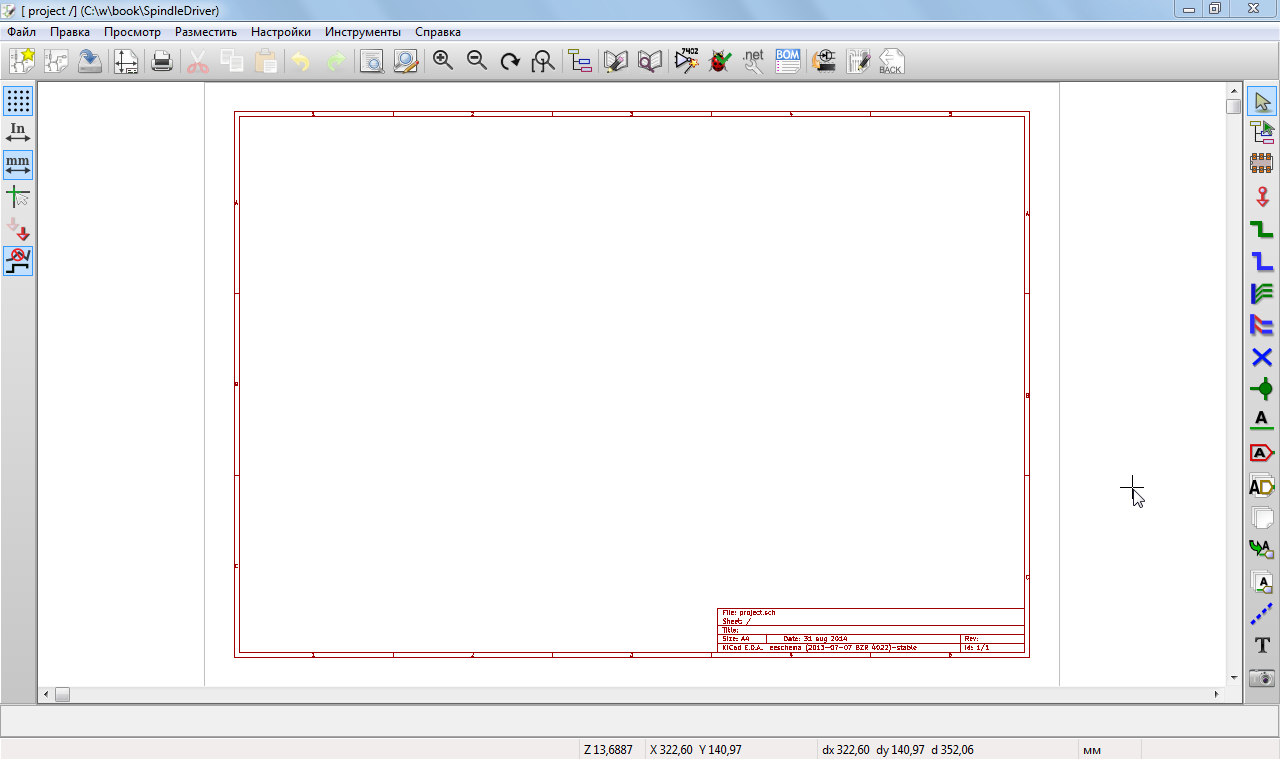
\includegraphics[width=0.9\textwidth]{kicad/ee15.png}

Завершение работы инструмента: вы можете выбрать другой инструмент из правой
инструментальной панели или же указать \menu{Отложить инструмент} по правому
клику мышки \keys{\rms}.

\section{Инструмент \emph{Добавить компоненты}}

\begin{itemize}
  \item 
На правой панели нажмите кнопку \menu{Разместить компонент}\
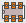
\includegraphics[height=2em]{kicad/ee21.png}. Курсор изменится со стрелки на
карандаш. Удобнее использовать сочетание клавиш \keys{Shift+A}.
Кликните в поле схемы чтобы начать размещение компонента. Появится диалог
\menu{Выбор компонента}. Вы можете выбрать компонент несколькими путями:
  \item
  \begin{enumerate}
    \item 
Если вы знаете точное имя копонента, введите его в поле \menu{Имя}, а
затем нажмите \keys{Enter} или \keys{OK}.
    \item 
Если вы знаете имя только приблизительно, в поле \menu{Имя} введите шаблон для
поиска, например, \menu{*BD*}, затем нажмите \keys{Enter} или \keys{OK}. Вы
увидите окно \\\menu{Выбрать компонент} со списком найденных компонентов.

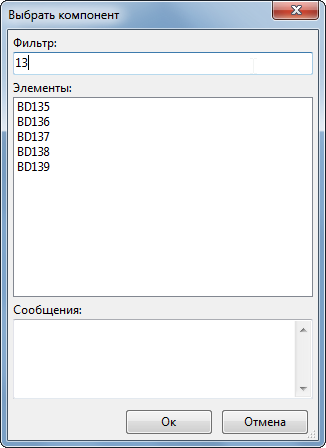
\includegraphics[height=0.5\textheight]{kicad/ee16.png}
    \item 
Вы можете искать компонент по ключевому слову, введя его в поле \menu{Имя},
затем кликнув \menu{Поиск по ключевому слову}. Однако на данный момент качество
библиотек все еще низкое, и немногие компоненты имеют ключевые слова, поэтому
эта возможность полезна косвенно.
    \item 
Можно выбрать недавно использованные компоненты из \menu{Списка истории}.
    \item 
Кнопка \menu{Список всех} вызывает диалог, в котором можно выбрать сначала
библиотеку \menu{74xx}, а затем ее компонент \menu{74HCT04}.
    \item 
Кнопка \menu{Выбор просмотром} вызывает \menu{Обзор библиотек}, позволяя
просмотреть библиотеки и находящиеся в них условные графические изображения.

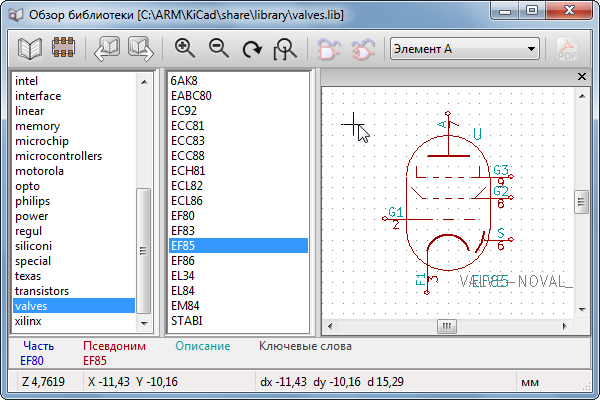
\includegraphics[height=0.5\textheight]{kicad/ee19.png}

  \end{enumerate} 
\end{itemize}

Вы также можете
вызвать обозреватель библиотек кнопкой\\
\menu{Просмотр библиотек и
компонентов}\ 
\includegraphics[height=2em]{kicad/ee20.png}

Выбрав элемент \dblms, вставьте символ в нужное место схемы \lms.
Позже вы сможете переместить его если нужно.
Зеркальное отражение компонента можно произвести следующим образом:

\begin{itemize}
  \item Поместите курсор на компоненте.
  \item По \rms\ выберите \menu{Ориентация компонента>Отражение}. 
  \item Без использования \term{контекстного меню}\ --- наведите мышь на
  компонент и нажмите кнопку \keys{X}\ или \keys{Y}.
\end{itemize}




\secrel{\prog{eeschema}: редактор электрических схем}

обеспечивает:

\begin{itemize}
\item создание однолистовых и иерархических схем,
\item проверку их корректности ERC (контроль электрических правил),
\item создание списка электрических цепей netlist для редактора топологии платы
pcbnew или для spice-моделирования схемы, 
\item доступ к документации на используемые в схеме электронные компоненты
(datasheet).
\end{itemize}


\secrel{Библиотеки компонентов}\secdown

\cp{http://habrahabr.ru/post/197582/}\bigskip

Модель компонента в САПР EDA состоит из следующих частей:

\begin{itemize}
  \item условное графическое обозначение (УГО) для схемного редактора
  \item модель компонента для редактора печатных плат (ПП)
  \item модель для симулятора (SPICE)
  \item 3D модель для передачи в универсальный САПР для работы с конструкцией
  \item дополнительные пользовательские данные: индексы компонента для
  заказа у разных поставщиков, ссылки на документацию, и т.п.
\end{itemize}

Части могут иметь несколько вариантов, например два варианта УГО (ГОСТ и ISO),
три корпуса (DIP, PLCC и LQFP), две модели для симулятора (идеальная и с
учетом паразитных эффектов), и 2 механических модели (габаритный кубик, и
подробная).

Кроме того, часто в один корпус упаковывается несколько одинаковых или разных
элементов. Одинаковые\ --- 2--4 операционных усилителя (ОУ), или вентили
логики. Разные\ --- части вакуумной лампы, разнесенные на схеме по разным
каскадам.

\bigskip

В составе KiCad поставляются библиотеки электронных компонентов (обычных и
поверхностно монтируемых SMD). Для многих библиотечных компонентов есть
3D-модели, созданные в \prog{Wings3D}.

Но как только вы начинаете работать со свежеустановленным KiCADом, тут же
обнаруживается, что библиотечные компоненты или не подходят\note{например не
соответствуют ГОСТ или стандартам предприятия}, или нужных компонентов попросту
нет в библиотеках.

Рассмотрим последовательное создание совершенно нового элемента на примере
модуля USB интерфейса HEX\_FT2232RL \ref{HEXFT2232RL}

\secrel{Создание УГО для схем}

Нам необходим встроенный редактор символов схем (библиотечных компонентов),
запускаем его следующим образом:

\begin{enumerate}
  \item Вначале запускаем \file{eeschema}
  \begin{itemize}
    \item[вверху] меню и панель инструментов
    \item[слева] область размерности и шага сетки редактора (настройка рабочей
    области)
    \item[справа] область элементов схем и перемещения по иерархии схемы
  \end{itemize}
  \item Далее запускаем встроенный
  \menu{Редактор библиотек}\ 
\includegraphics[height=2em]{kicad/ee22.png}

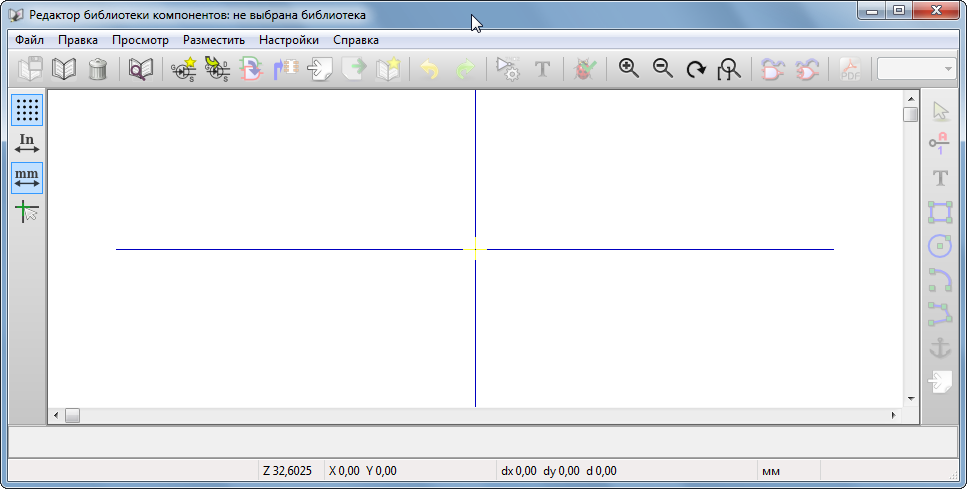
\includegraphics[height=0.5\textheight]{kicad/lib23.png}
\end{enumerate}

Необходимо создать новую библиотеку и первый собственный компонент:

\menu{Создать новый компонент}
\includegraphics[height=2em]{kicad/newel.png},

\menu{Свойства компонента>Общие Настройки},

\menu{Имя компонента>HEX\_FT232RL}

\menu{Обозначение по умолчанию>U}

\menu{Количество элементов в корпусе>1}

\menu{OK}
\bigskip

В верхней панели инструментов активировались несколько кнопок, выбираем

\menu{Сохранить текущий компонент в новой библиотеке}

\includegraphics[height=2em]{kicad/lib26.png}

В открывшемся диалоге выберите каталог для библиотеки
\file{/home/user/kicad/}, и укажите имя файла (новой) библиотеки
\menu{\file{MyModules}>Сохранить}.

\bigskip
Теперь нужно добавить созданную библиотеку в рабочий список.
\bigskip

Настроим дополнительный путь, где лежат файлы библиотек. Это могут быть ваши
личные библиотеки, специальная библиотека для конкретного проекта, или комплект
библиотек поставляемых вместе с этой книгой: выберите в меню
\menu{Настройки>Библиотека}, \menu{Пользовательские пути
поиска>добавить>\file{/home/user/kicad/}}, \menu{Ok}.

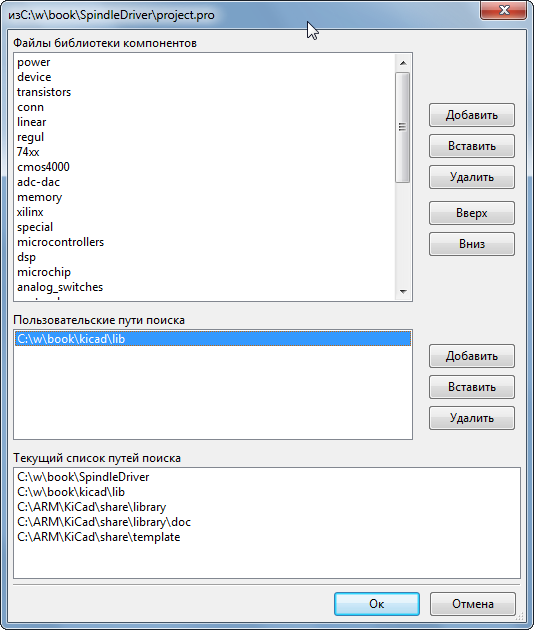
\includegraphics[height=0.5\textheight]{kicad/lib25.png}

\menu{Настройки>Библиотека},
\menu{Файлы библиотеки компонентов>power>\lms>Вставить}.
Выбираем только что созданную библиотеку \file{MyModules}.
Она будет вставлена в список до выбранной \file{power}.

\bigskip
Проделанные настройки применятся только к текущему проекту. Если Вы хотите 
чтобы новая библиотека всегда добавлялась к новым проектам, вам нужно добавить
новый путь поиска библиотек и ее название в файл шаблона, как это описано в
\ref{kicadtemplates}.

\bigskip
Если вы хотите изменить только что созданное или уже сущесствующее УГО, нужно
выбрать рабочую библиотеку, ту библиотеку в которой мы хотим работать (создавать
или редактировать компоненты). На панели инструментов нажимается кнопка

\menu{Выбор рабочей библиотеки}
\includegraphics[height=2em]{kicad/lib24.png},

\menu{Выбрать библиотеку>MyModules>Ok}.

Загружаем созданный ранее (пустой) компонент \file{HEX\_FT232RL} (или любой
другой)

\menu{Загрузить компонент для редактирования}
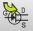
\includegraphics[height=2em]{kicad/editel.png}

\menu{Выбор компонента>Список всех>Элементы>\file{HEX\_FT232RL}>Ok}

\bigskip
\includegraphics[height=0.45\textheight]{odurino/usb/HEXFT232RL.png}

Сейчас у нас элемент не имеет графических элементов, и состоит только из
нескольких текстовых полей с обозначениями, слепленных в одной точке. Нужно их
растащить: \rms, САПР не может различить близкие элементы и уточняет для
какого поля мы хотим контекстное меню. Выбираем любое, \menu{Переместить поле}\
или кнопка \keys{M}. Перетаскиваем элемент, и \lms\ на свободном месте.

Пользуясь \ref{eskd}, отрисовываем на освободившемся месте УГО элемента,
пользуясь кнопками на панели справа. Рисование выполняется по сетке, шаг
выбирается \menu{\rms>Выбор сетки}, набор сеток фиксированный (?). При рисовании
ГОСТовских УГО округляем до ближайших дюймовых размеров\footnote{\ 1mil=1/1000
дюйма, 100mil=2.54mm=типовой шаг DIP микросхем}, или в меньшей сетке если нужно
точно гостовские размеры.

УГО имеет \term{точку привязки}, относительно которой отрисовываются элементы.
На практике важно то, что вокруг этой точки элемент вращается. Для перемещения
этой точки можно использовать кнопку

\menu{Переместить точку привязки}
\includegraphics[height=2em]{kicad/lib27.png}.

Добавляем выводы компонента: \menu{Добавить вывод
компонента}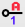
\includegraphics[height=2em]{kicad/lib28.png}.

\bigskip
Например для резистора создание выводов будет выглядеть вот так:

\bigskip
\menu{Свойства вывода}

\menu{Имя>A}

\menu{Номер>1}

\menu{Ориентация>Вправо}

\menu{Электр.тип>Пассивный}

\menu{Размер шрифта>1.27мм}

\menu{Длина>2.54мм}

\menu{Ok}

\bigskip

\menu{Имя>B}

\menu{Номер>2}

\menu{Ориентация>Влево}

\menu{Ok}

\bigskip
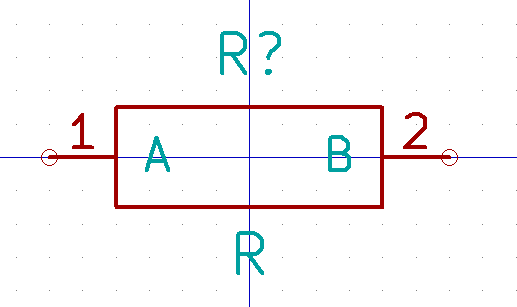
\includegraphics[height=0.5\textheight]{kicad/lib29.png}
\bigskip

Сохраняем библиотеку: \menu{Сохранить текущую
библиотеку}
\includegraphics[height=2em]{kicad/lib30.png}

\menu{Подтверждение>Включая последние изменения компонента?>Да}

\menu{Подтверждение>Компонент существует. Изменить его?>Да}

\menu{Подтверждение>Изменить файл библиотеки ?>Да}

\secrel{Модель печатной платы}

Модель печатной платы в программе \pcbnew\ состоит из нескольких
\termdef{слоев}{слой печатной платы} с разными функциями, для типичной
двухслойной ПП:

\begin{itemize}
  \item верх
  \begin{description}
  \item[Front] медь верхнего слоя
  \item[Adhes\_Front] карта нанесения клея для компонентов
  \item[SoldP\_] карта нанесения паяльной пасты
  \item[SilkS\_] шелкография: маркировка элементов, надписи, и т.п.
  \item[Mask\_] паяльная маска 
  \end{description}
  \item низ
  \begin{description}
  \item[Back] медь нижнего слоя
  \item[Adhes\_Back] карта нанесения клея для компонентов 
  \end{description}
  \item контуры
  \begin{description}
  \item[Контур ПП] слой определяющий физ.геометрию платы, используется при
  фрезеровке контуров, сверлении монтажных отверстий, разделке сверловкой и т.п.
  \item[Пояснения] вспомогательная текстовая информация
  \item[Чертеж] вспомогательная графическая информация: габаритные размеры, зоны
  монтажа,..
  \end{description}

\item В зависимости от технологии производства и пожеланий разработчика могут
добавляться любые дополнительные слои.
\end{itemize}

\secrel{Создание падстека}

\termdef{Падстек}{падстек}\ --- модель контактной площадки компонента, в виде
набора геометрий отдельно для каждого \term{слоя} печатной платы. Также включает
информацию о диаметре сверления.

% \secrel{PS:}
% 
% Компоненты и посадочные места корпусов можно ассоциировать с документацией,
% ключевыми словами и осуществлять быстрый поиск компонента по функциональному
% назначению.
% 
% \secup
% 
% \secru{Отрисовка схемы (часть 2)}
% 
% \secdown
% 
% \secru{Автоматическое обозначение элементов}
% 
% Автоматическое обозначение элементов и перенумерация выполняется кнопкой\\
% \menu{Обозначить компоненты на
% схеме}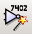
\includegraphics[height=2em]{kicad/ee000004.png}
% 
% \secru{Генерация списка цепей}
% 
% Список цепей (нетлист) используется для передачи информации о соединении
% компонентов между программами. Чаще всего СЦ создается после отрисовки схемы для
% передачи данных в программу трассировки печатной платы (ПП).

\secup


\secrel{\prog{gerbview}: просмотр фотошаблонов}

позволяет просматривать Gerber-файлы перед передачей печатных плат в
производство.


\section{Программа \prog{Wings3D} для создания 3D моделей}

Эта программа может вам пригодиться если вы планируете создавать 3D модели для PCB элементов.

Архив и файлы документации (Linux и Windows) в папке kicad/wings3d.

Взгляните на домашнюю страницу Wings3D чтобы узнать подробнее о программе.

pcbnew использует файлы в формате wrml (.wrl) экспортируемые из Wings3D (родной формат Wings3D - это .wings).

\subsection{Установка \prog{Wings3D} под \win}

\menu{\winr{\url{http://www.wings3d.com/}}>Downloads>Stable Release>\win
(32/64b)}

\menu{file{wings-n.n.n.exe}}

\menu{Compononets>\checkbox QuickLaunch>Next}

\menu{Location>\file{C:/Program Files/wings3d\_n.n.n}>Next>Install>Close}% 



% \secrel{Расчет схем и моделирование в \ngs}\label{spice}\secdown
% \secdown

на основе статьи

\cp{http://www.mithatkonar.com/wiki/doku.php/kicad/kicad\_spice\_quick\_guide}

\cp{http://physics.gmu.edu/~rubinp/courses/407/ngspice.pdf}

Electronic circuit simulation with gEDA and NG-Spice by Example

\copyright\ Andreas Fester

\bigskip

\prog{\spice}: [S]imulation [P]rogram with [I]ntegrated [C]ircuit
[E]mphasis\ --- пакет программ симуляции и расчета электронных схем,
была создана для моделирования \emph{интегральных микросхем}, расчета режимов
работы, оптимизаии, и предсказания поведения.

\bigskip
\spice\ может выполнять несколько видо схемотехнических расчетов, самые важные
из которых:

\begin{itemize}
  \item
Нелинейный анализ по постоянному току: вычисление передаточной характеристики по
постоянному току
  \item
Нелинейный анализ переходных процессов: вычисление токов и напряжений как
функции времени в условиях большого сигнала
  \item
Линейный AC анализ: вычисление выхода как функции от частоты. Выводится
\term{bode plot}
  \item
Анализ шума
  \item
Расчет чувствительности
  \item
Анализ искажений
  \item
Фурье-анализ: вычисление и отображение частотных спектров
  \item
Анализ Монте-Карло
\end{itemize}

\bigskip

\secrel{Доступные SPICE-пакеты}\secdown

Первоначально \spice\ был разработан в Университете Беркли. Другие версии
\spice\ являются форками этой реализации, и сейчас существует несколько
вариантов:

\begin{itemize}
\item \href{http://ngspice.sourceforge.net/}{\ngs}: самый доступный
бесплатный OpenSource SPICE-движок.
\item \url{http://www.ngspice.com/}\ --- on-line вариант \prog{ngspice}, удобен
для начального обучения
\item \href{http://www.linear.com/designtools/software/}{\lts}:
Популярная бесплатная коммерческая версия от Linear Technology для \win.
Работает в \prog{WINE}. Поставляется в комплекте с графической оболочкой,
но требуется проверка файлов расчетных заданий, которые она создает.
\item
\href{https://www.gnu.org/software/gnucap/}{gnucap}\note{уже включен в
виндозную сборку KiCAD}:
Не совсем SPICE, но пытается быть синтаксически совместмой.
\item \href{http://www.spiceopus.si/}{SpiceOpus}: Коммерческая, но
удобная, особенно в плане вывода графиков.
\item
\href{http://www.cadence.com/products/orcad/pspice_simulation/Pages/default.aspx}{PSpice}:
\win-only, дорогой коммерческий пакет, стандарт de-facto для
профессионального применения в USA в составе тяжелых EDA-продуктов.
Они традиционно предоставляют обрезанную \emph{gratis}-версию для студентов.
Также имеет в комплекте GUI.
\item \prog{MultiSim}, \prog{OrCAD}, \prog{DesignLab},.. коммерческие
EDA-пакеты, содержит в составе одну из версий \prog{P\spice}
\item Какие-то еще?
\end{itemize}

В этом разделе описан \ngs, который был написан с целью полностью переписать
оригинальную реализацию Беркли \spice. Сейчас он все еще содержчит часть кода
Беркли, но в этом коде было исправлено множество ошибок.
Важно пониать, что каждая реализация \spice\ может вести себя особенно в
некоторых случаях: некоторые из них более совместимы между собой, другие менее.
Всегда важно прочитать документацию, которая поставляется с конкретной
версией \spice. Дистрибутив \ngs\ пославляется с детальным руководством
пользователя, а этот раздел поможет вам начать. Хорошо иметь под рукой полное
руководство при чтении этого раздела, так как интересующие вас команды там
рассмотрены детальнее.

\secrel{Установка \ngs\ под \win}

\menu{\winr\url{http://ngspice.sourceforge.net/download.html}>\prog{ng-spice-rework}>\file{ngspice-xx\_xxxxxx.zip}}

\menu{unzip \file{ngspice-xx\_xxxxxx.zip}>\file{C:/spice}}

\menu{\winstart>Компьютер>\rms>Свойства>Дополнительные
параметры системы}

\menu{Переменные среды>\file{PATH=\ldots;C:/spice/bin}}

\secrel{Установка \lts\ (только \win)}

\menu{\winr>\url{http://www.linear.com/designtools/software/}}

\secrel{Установка \ngs\ под \linux}

\begin{verbatim}
root# aptitude install ngspice
\end{verbatim}

Пакет \pack{\ngs}\ также может быть легко собран и установлен компиляцией
их исходниов. После загрузки архива, соберите пакет для вашего дистрибутива:
\begin{verbatim}
tar xvzf ng-spice-rework-15.tgz
 cd ng-spice-rework-15
./configure --with-readline=yes
make
checkinstall
\end{verbatim}

Убедитесь что в системе присутствует библиотека \pack{GNU readline}, и она
включена в опциях \prog{configure}: ее использование делает интерфейс командной
строки более комфортным. Подробнее сборка \ngs\ описана в его руководстве в
составе дистрибутива.

\bigskip
Сборка \ngs\ для az\linux\ описана в разделе \ref{azspice}.

\secup

\secrel{Пошаговый пример использования}

Рассмотрим очень простой пример симуляции электронной схемы. В основном вы
будете рисовать ваши схемы в \eeschema, но интерактивная симуляция пока не
реализована.

\secdown

\secrel{Рисуем схему в \kicad}

Схема, которую мы хотим рассчитать\ --- простой \term{RC-фильтр}. Эта схема была
выбрана, так как она содержит очень ограниченное количетво элементов, и поэтому
понятна: источник напряжения, резистор и конденсатор. Использование редактора
схем вам уже должно быть знакомо из предыдущего раздела (\ref{eeschema}).
Запустите \eeschema\ и нарисуйте схему:

\bigskip
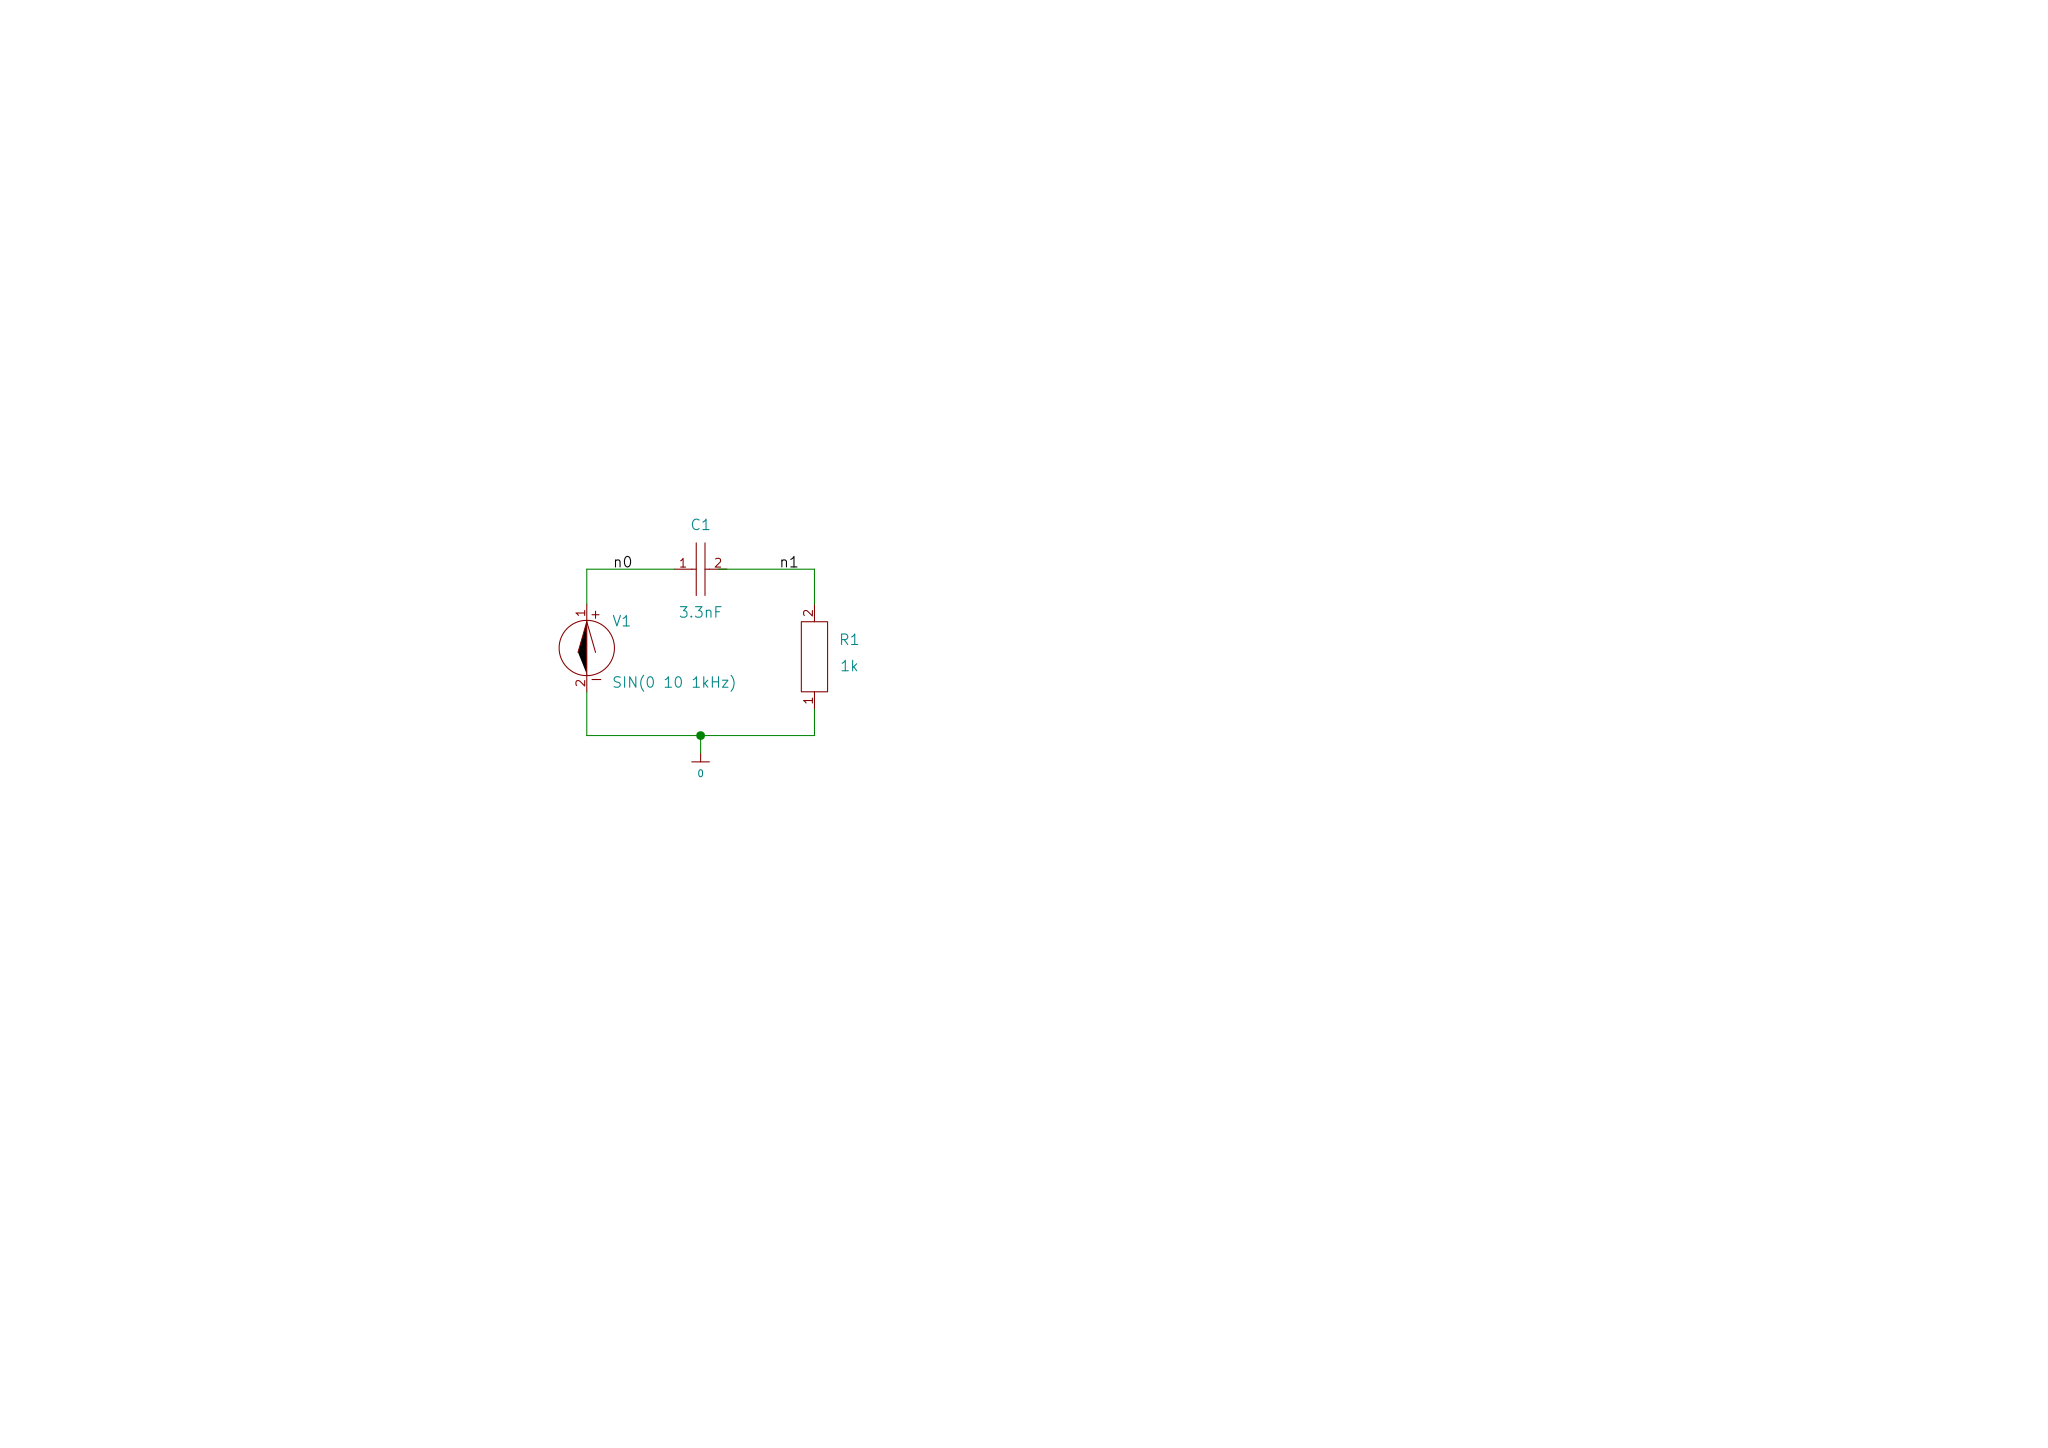
\includegraphics[height=0.5\textheight]{spice/RCfilter.pdf}
\fig{figspicerc}{Простой RC-фильтр}
\bigskip

Имена, указанные на проводниках\ --- \emph{имена цепей}. Они могут не
указываться, если вам не нужно на них ссылаться в расчете. При экспорте списка
цепей из \eeschema\ им будут присвоены униальные имена. Цепь может иметь любое
имя, за некоторым исключением: \emph{в списке должна быть одна цепь с именем
[\elem{0}], она подключается к общему проводу (земле)}. Рисуя схему, поместите
на нее один или несколько элементов [\elem{0}]\ из библиотеки \file{spice}.

\elem{V1}\ --- \term{независимый источник напряжения}. Его значение задано в
виде выражения \verb|SIN(0 10 1kHz)|, создающего синусоидальный (SIN) сигнал со
смещением (0)\,вольт, амплитудой (10)\,вольт и частотой (1kHz).

\bigskip
Рисуйте вашу схему, соблюдая несколько рекомендаций:
\begin{itemize}
  \item
Для именованных цепей используйте \emph{глобальные метки} вместо локальных.
В списке цепей глобальные идентификаторы цепей включаются как есть, а
локальные метки модифицируются, что делает сложным последующие ссылки на них при
SPICE-моделировании.
  \item
Используйте компонент [\elem{0}] из библиотеки \file{spice}, вместо обычного
комопнента [\elem{GND}]: ”\elem{0}” официальное имя главной земли в файлах
P\spice. Некоторые \spice-движки умеют транслировать $GND \rightarrow 0$, другие
нет.
\end{itemize}

\secrel{Создание списка цепей}

Входными данными для симуляции является \term{список цепей (netlist)}.
Список цепей создается через экспорт из \eeschema. Если
вы используете программу рисования схем, посмотрите в ее документации, умеет ли
она экспорт в \spice (\file{.cir}), и как это сделать.

\begin{itemize}
  \item
Кликните кнопку или пункт меню \menu{Сформирвать список цепей}.
  \item
Выберите вкладку \menu{Spice}, и убедитесь что включен крыжик \menu{\checkbox\
Формат по умолчанию}. Вам нужно сделать это только один раз, настройки
запоминаются.
\item
Нажмите кнопку \menu{Сформировать}
\end{itemize}

Если вы хотите запускать \ngs\ из диалога экспорта:
\begin{itemize}
  \item
Заполните полный путь с программе симуляции, типа
\file{C:/spice/bin/ngspice.exe} со всеми путями и расширениями, \kicad\ пока не
научился запускать симулятор через \verb|PATH|.
  \item
Нажмите кнопку \menu{Запустить симулятор}.
\end{itemize}

\bigskip
В результате экспорта будет создан файл

\lst{RCfilter.cir}{}{spice/RCfilter.cir}

Формат нетлиста \spice\ прост: каждая строка содержит один элемент схемы.
Первый столбец каждой строки содержит имя элемнта, затем идут имена цепей,
которым подключен каждый вывод, последним идет значение элемента.
Строки, наначинающиеся с [*]\ --- комментарии.
В нашем примере строка, начинающаяся с \elem{V1}, описывает источник напряжения,
подключенный к цепям \elem{n0} (вывод 1) и \elem{0} (вывод 2), значение
\verb|SIN(0 10 1kHz)|. Точно также заданы конденсатор и резистор. Так как цепи
\elem{n0,n1}\ заданы именами, перед ними стоит [/].

Первая и последняя строки имеют для \ngs\ особое значение: при чтении нетлиста
\ngs\ считает первую строку названием схемы. Последняя строка должна содержать
токен \elem{.end}.

Так как формат файла нетлиста настолько прост, его можно легко создать вручную
из любого текстового редактора. Некоторые статьи о \spice-симуляции даже
начинаются с такого способа, но он действительно неудобен для работы. Используя
\eeschema\ или другой редактор схем, намного проще изменять схему, и она может
быть легко распечетана или включена как иллюстрация в документацию. Единственный
реальный вариант, когда нужно работать напрямую в файлом\ --- если вам вдруг
понадобиться сформировать его автоматически, например при анализе паразитных
емкостей и индуктивностей печатной платы, которые определяются формой печатных
проводников.

\secrel{Запуск симуляции}

Теперь вы готовы симулировать схему. Прежде всего нам нужно решить, какие виды
расчетов, которые умеет делать \spice, нас интересуют:

\begin{itemize}
  \item \term{Анализ переходных процессов}\ показывает поведение
  схемы во времени.
  \item \term{Расчет по переменному току (AC)}\ дает измененения работы схемы с
  изменением (входой) частоты.
  \item \term{Параметрическая симуляция}\ позволяет анализировать изменения в
  работе схемы при изменении одного или нескольких параметров, например
  изменении частоты источника и емкости конденсатора.
\end{itemize}

Для начала посмотрим как ведет себя входное напряжение во времени. Мы хотим
выполнитьанализ переходных поцессов в схеме, и вывести напряжение между сетями
\elem{n0} и \elem{0}.

Запускаем \ngs:

\begin{verbatim}
$ ngspice

spinit found in c:\spice\share\ngspice\scripts\spinit
******
** ngspice-24 : Circuit level simulation program
** The U. C. Berkeley CAD Group
** Copyright 1985-1994, Regents of the University of California.
** Please get your ngspice manual from http://ngspice.sourceforge.net/docs.html
** Please file your bug-reports at http://ngspice.sourceforge.net/bugrep.html
** Creation Date: Jan 30 2012   22:58:51
******
ngspice 1 ->
\end{verbatim}

Теперь нам нужно загрузиь нетлист (выводится заголовок: первая строка файла):

\begin{verbatim}
ngspice 1 -> source RCfilter.cir

Circuit: * eeschema netlist version 1.1 (spice format) creation date: 26.12.2014 16:15:26
\end{verbatim}

Так как мы задали для входного напряжения частоту 1\,КГц, период
$T=1/F=0.001$\,с$=1$\,мс.
Мы хотим увидеть как входное наряжение меняется за первые 5 периодов, т.е.
5\,мс. Запускаем симуляцию следующей командой:

\begin{verbatim}
ngspice 2 -> tran 0.01ms 5ms
Doing analysis at TEMP = 27.000000 and TNOM = 27.000000

Warning: v1: no DC value, transient time 0 value used

Initial Transient Solution
--------------------------

Node                                   Voltage
----                                   -------
/n1                                          0
/n0                                          0
v1#branch                                    0

No. of Data Rows : 512
\end{verbatim}

Первый параметр \verb|tran| определяет \term{шаг расчета}, второй\ ---
\emph{конечное значение времени}. Если не указан третий параметр,
начальное время равно 0, иначе третий параметр указывает ненулевое
\emph{начальное время}. Ну, это все \smiley. Симуляция выполнена. Теперь нам
нужно увидеть результат симуляции.

\secrel{Просмотр результата расчета}

\spice\ создал таблицы с рассчитанными значениями: 512 значений для каждого узла
схемы. Для простого просмотра чисел выполним команду (не забудьте про кавычки,
без них не работает если первый символ [/]):

\begin{verbatim}
ngspice 3 -> plot "/n0"
\end{verbatim}

\clearpage
\noindent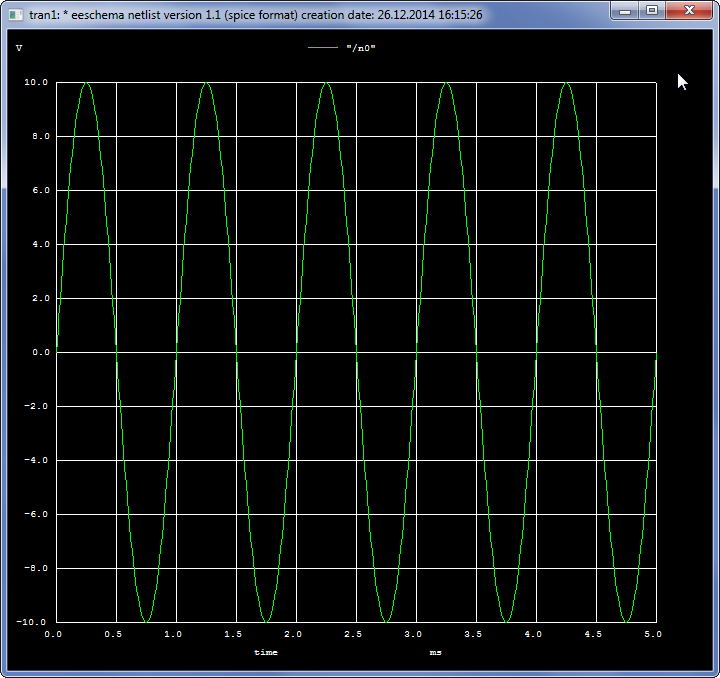
\includegraphics[height=\textheight]{spice/spice1.png}
\clearpage

Эта команда вывела напряжение при переходном процессе на цепи \net{n0}.

Как вы заметили, диаграмма сигнала отображается на черном фоне. Если вам нужны
другие цвета, например для вставки в документацию, их можно переопределить:

\begin{verbatim}
ngspice 12 -> set color0 = white
ngspice 13 -> set color1 = black
ngspice 14 -> set color2 = green
ngspice 3 -> plot "/n0"
\end{verbatim}

\noindent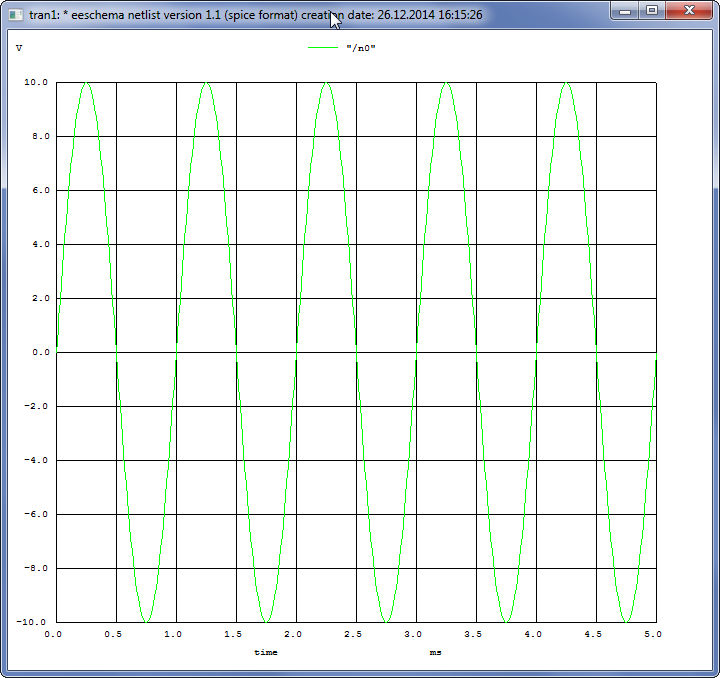
\includegraphics[height=0.5\textheight]{spice/spice2.png}

\bigskip
Диаграмма показывает форму входного сигнала, как мы и ожидали, но она нас мало
интересует, так как мы ее и задали. Нам интереснее например \emph{напряжение на
резисторе}, кроме того мы попробуем \emph{сравнить два сигнала}.
Это легко сделать указав два имени цепи:

\begin{verbatim}
ngspice 31 -> plot "/n0" "/n1"
\end{verbatim}

\clearpage
\noindent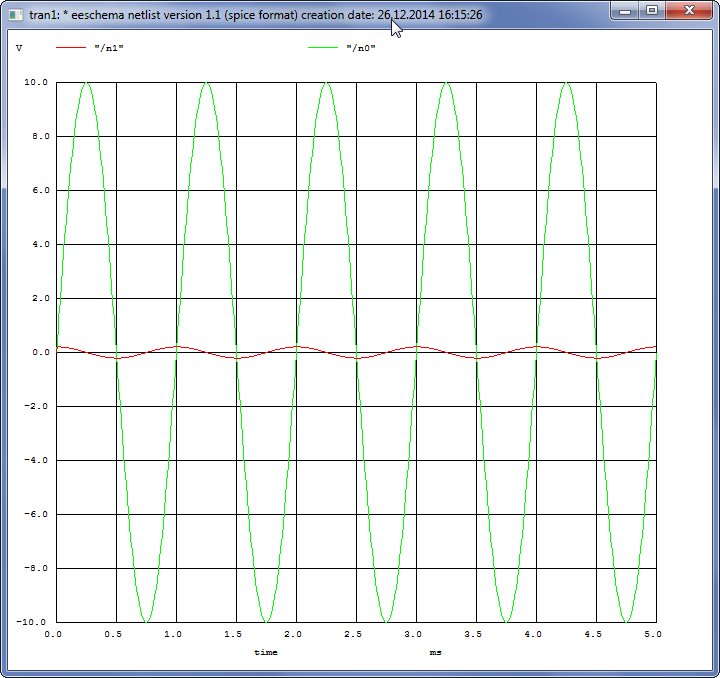
\includegraphics[height=\textheight]{spice/spice3.png}
\clearpage

\secrel{Расчет АЧХ по переменному току (AC симуляция)}

Сигнала на резисторе почти не видно. Теперь вопрос: какие частоты попускает наш
фильтр ? Для определения этого теперь выполним \term{расчет по переменному току
(AC симуляцию)}. Команда для этого \verb|ac ( DEC j OCT j LIN )N FStart FEnd|.

\verb|FStart| и \verb|FEnd|\ --- соответственно начальная и конечная частота.
Необязательные параметры \verb|DEC|, \verb|OCT| или \verb|LIN| указывают способ
изменения частоты: декадно, октавно или линейно. Если выборана октавная или
декадная \term{вариация частоты}, то параметр \verb|N| задает число
частот на декаду или октаву. Для выполнения \term{AC анализа} должен быть
изменен источни сигнала: сейчас он определен как синус с амплитудой 10\,В и
частотой 1\,КГц. Для анализа это должен быть \emph{источник переменного
апряжения}. Снова запускаем \eeschema\ и меняем значение источника:

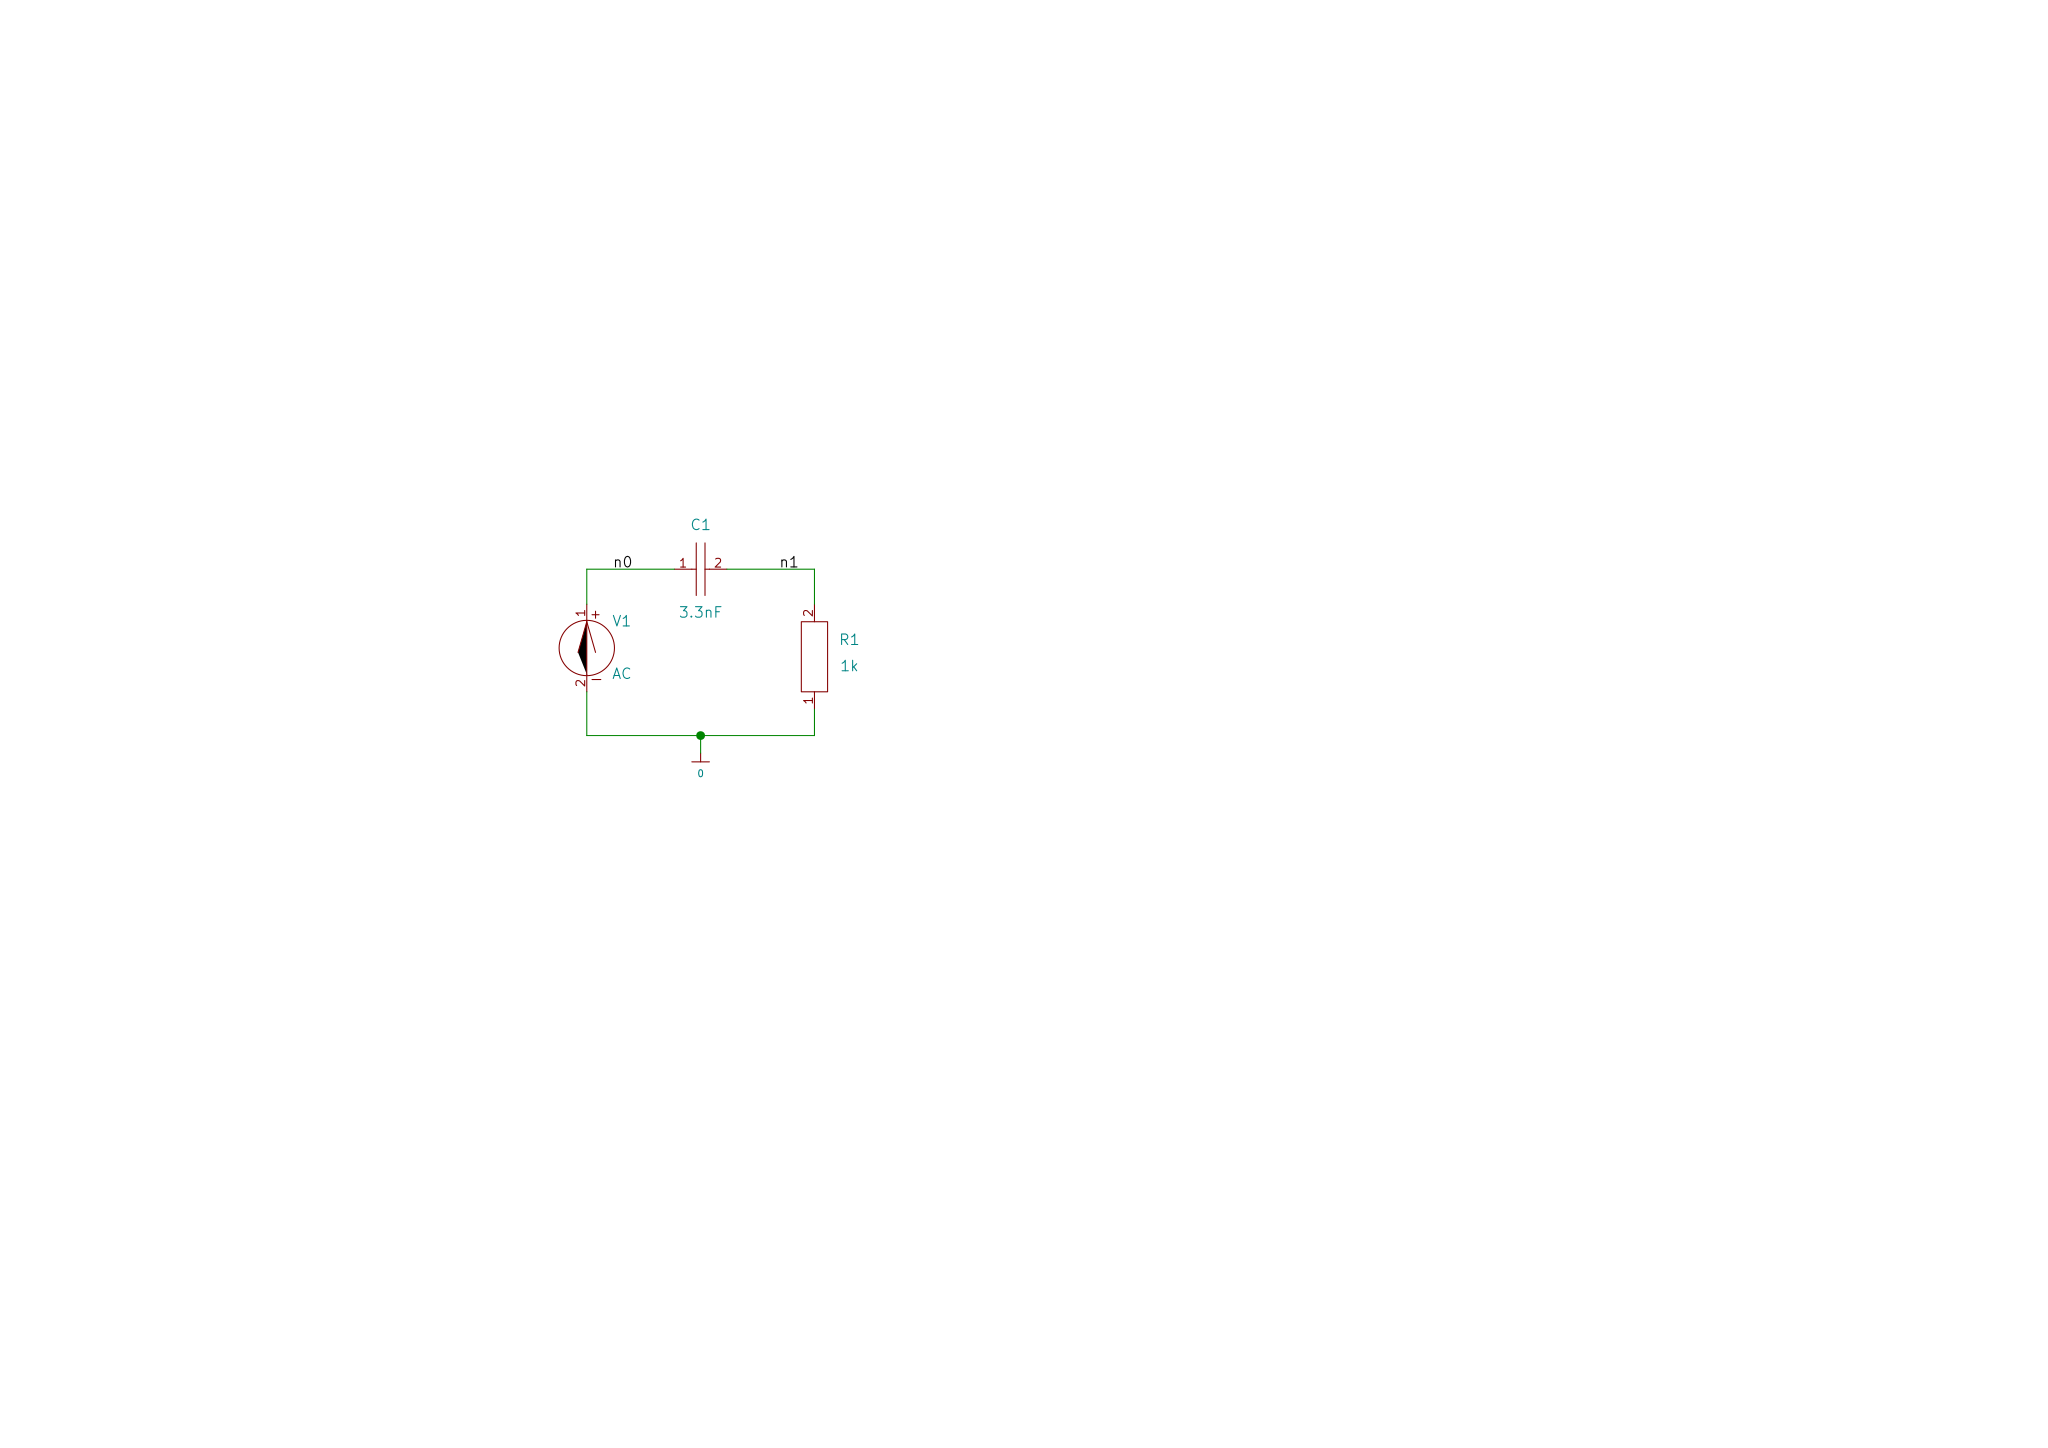
\includegraphics[height=0.5\textheight]{spice/ACanaliz.pdf}

Создаем нетлист, загружаем ео и запускаем команду AC анализа:

\begin{verbatim}
$ ngspice ACanaliz.cir
ngspice 1 -> ac lin 1000 0.1 250kHz
Doing analysis at TEMP = 27.000000 and TNOM = 27.000000

Warning: v1: has no value, DC 0 assumed


No. of Data Rows : 1000

ngspice 2 -> plot "/n1"
ngspice 3 -> plot "/n0" "/n1"
\end{verbatim}

Эта команда выполяняет \term{линейный AC анализ} от (почти) 0\,Гц до 250\,КГц.
Результат можно увидеть как напряжение для источника, так и напряжение на
\elem{R1}:

\pagebreak\noindent
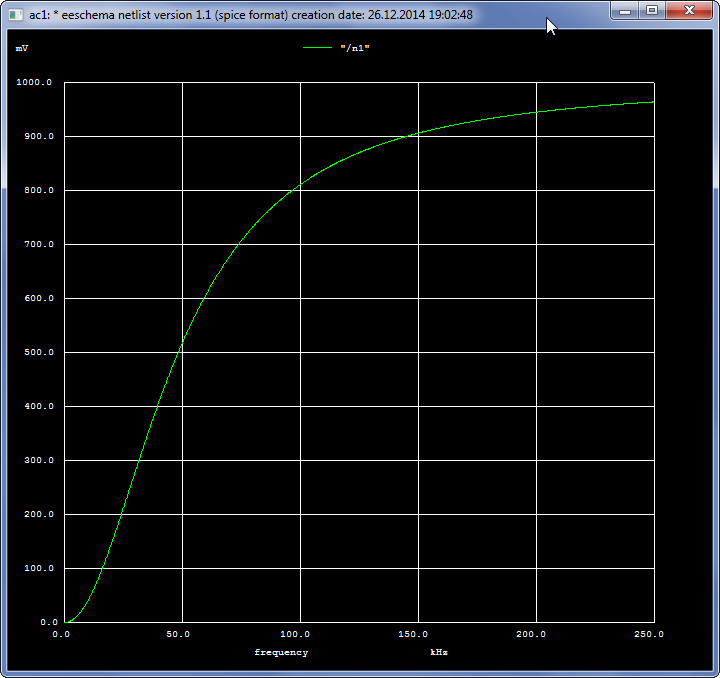
\includegraphics[height=\textheight]{spice/spice4.png}

\pagebreak\noindent
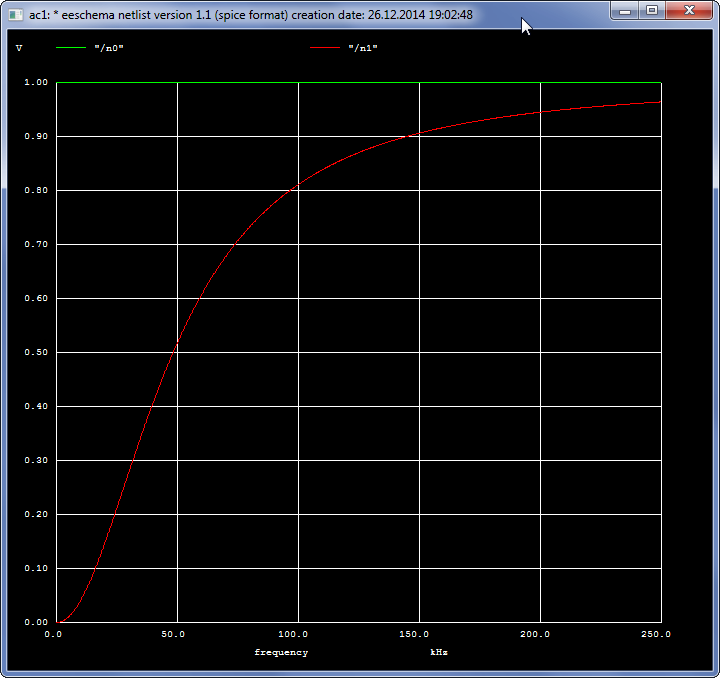
\includegraphics[height=\textheight]{spice/spice5.png}

\secrel{Симуляция полноволнового выпрямителя}

\noindent
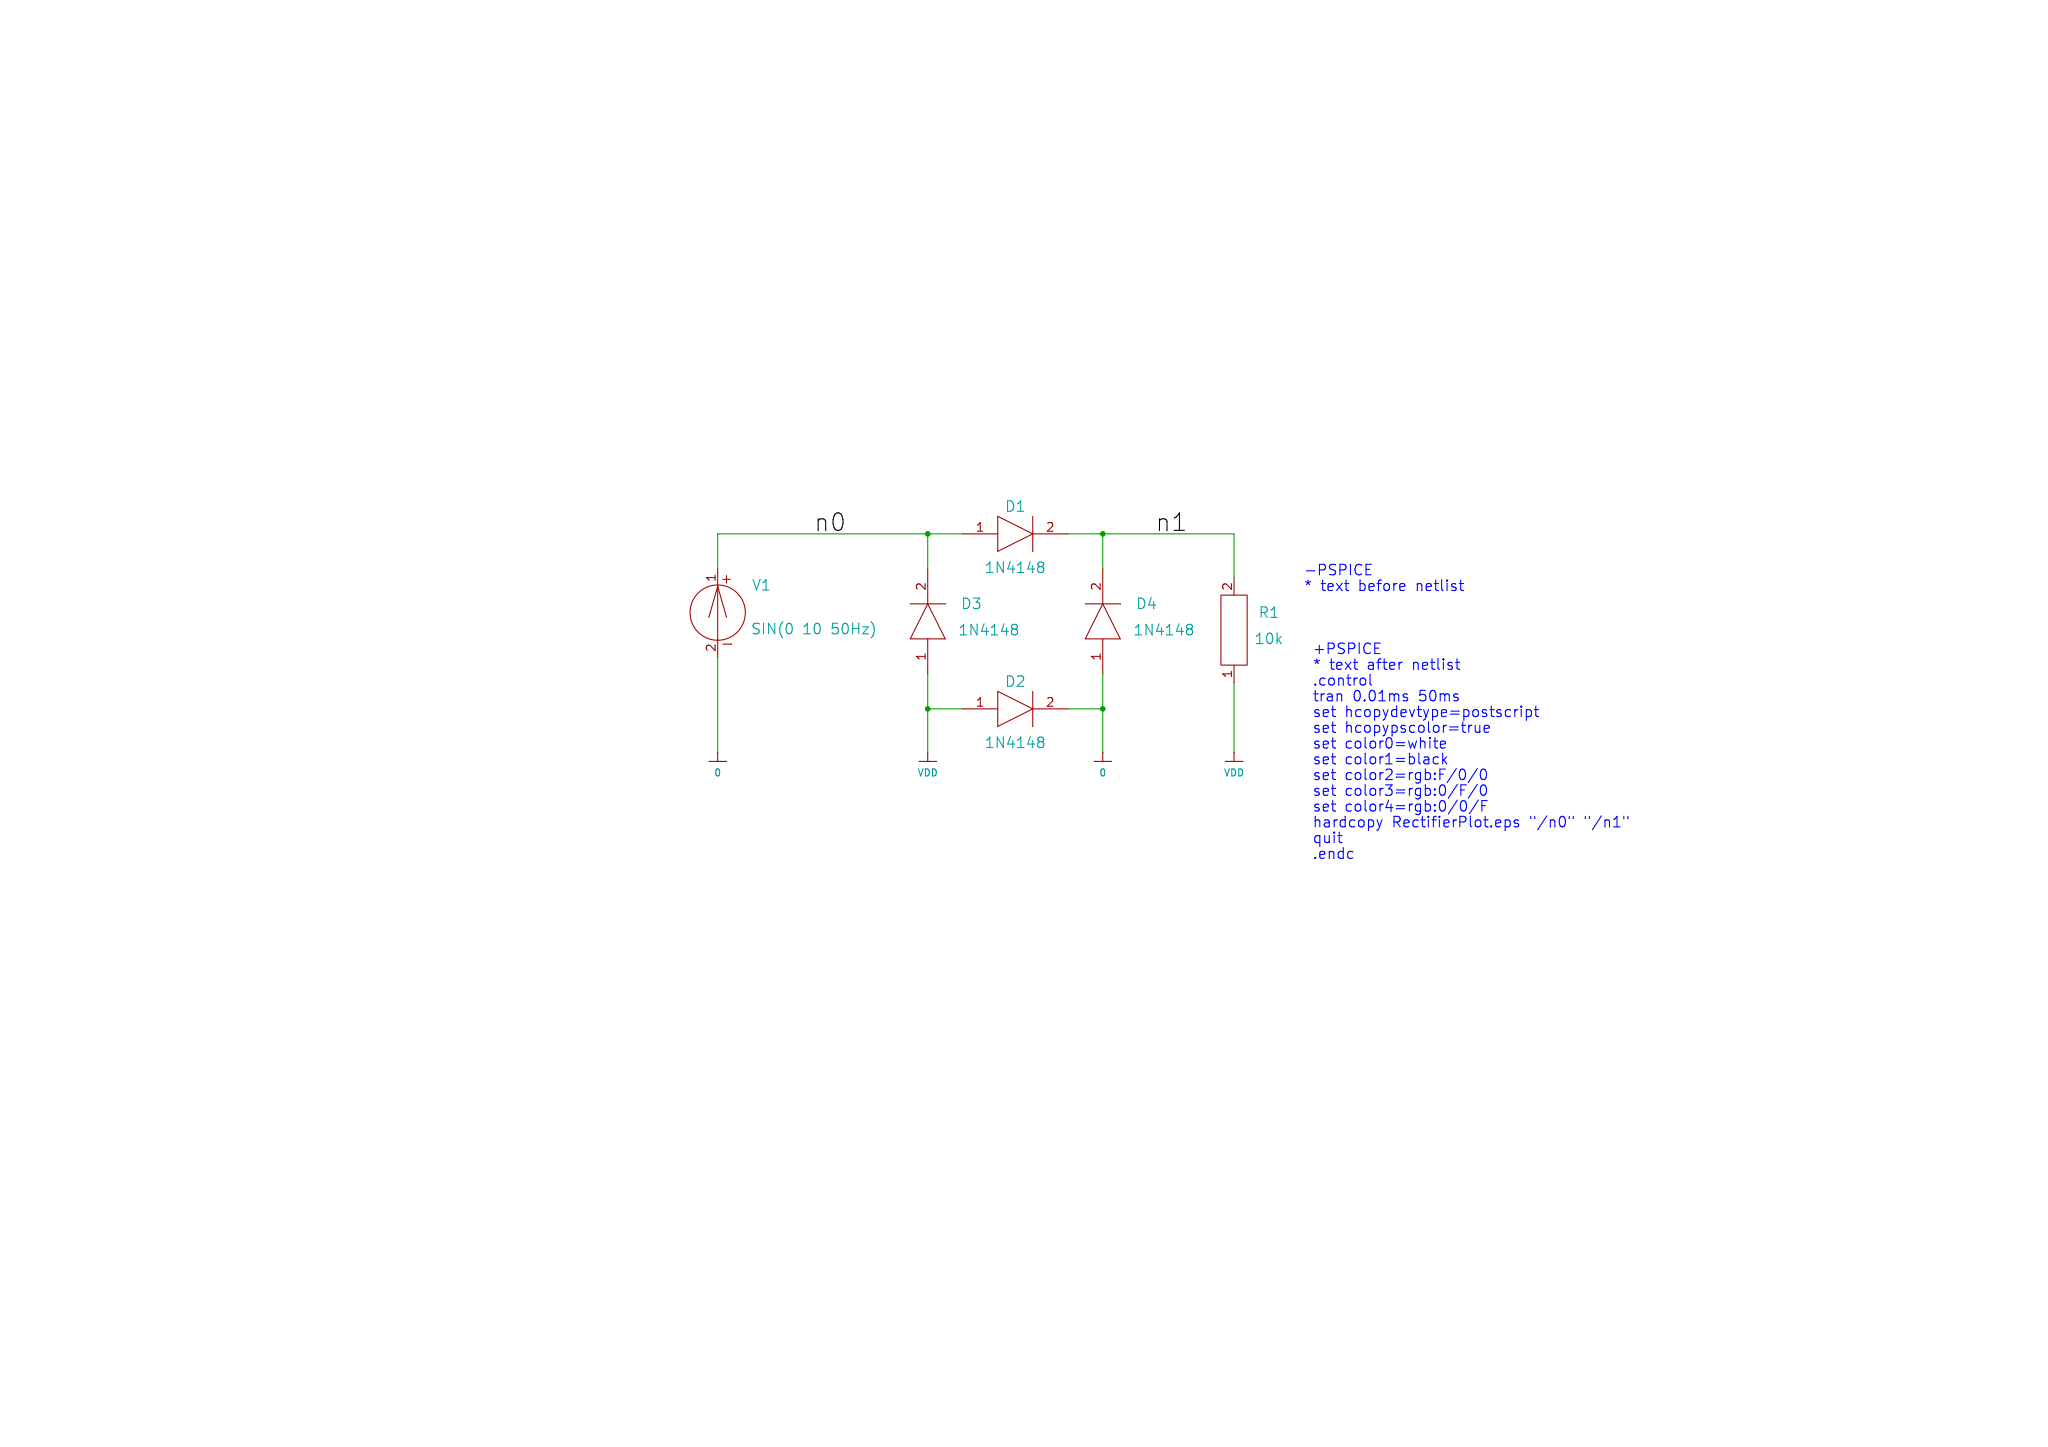
\includegraphics[height=0.5\textheight]{spice/Rectifier.pdf}

\lst{Rectifier.cir}{}{spice/Rectifier.cir}

\pagebreak\noindent
\includegraphics[height=\textheight]{spice/rectifierplot.eps}

% % In the following sections, we are going to simulate more circuits to get
% better involved with NG-spice.
% % 4 Simulating a full wave rectier
% % 1
% % +
% % 2
% % -
% % V1
% % SIN(0 10 50Hz)
% % D1
% % 1N4148
% % n0
% % R1
% % 10k
% % n1
% % 0
% % D2
% % 1N4148
% % D3
% % 1N4148
% % D4
% % 1N4148
% % Vdd Vdd
% % Figure 6: A full wave rectier.
% % Figure 6 shows the typical full wave rectier circuit. Both half waves of the input signal can be used, i.e.
% % the negative half wave is mirrored upwards. This can be seen in Figure 7 which shows the spice simulation of
% % the circuit.
% % time
% % 0.0 5.0 10.0 15.0 20.0 25.0 30.0 35.0 40.0 45.0 50.0
% % ms
% % -10.0
% % -5.0
% % 0.0
% % 5.0
% % 10.0
% % V v(n1,vdd) tran.v(n0)
% % Figure 7: Source voltage transient and voltage across R1
% % 
% % \secrel{Links to useful resources}
% % 
% % URLs
% % [1] , TBD <http://www.ecircuitcenter.com/>.
% % [2] , GPL Electronic Design Automation <http://geda.seul.org>.
% % [3] , TBD <gnucap> .
% % [4] , TBD <gwave> .
% % [5] , NG-SPICE: The free circuit simulator <http://www.ngspice.org>.

\secup
\secup


% % \chapter{FreeCAD}

\section{Чертеж}

\section{Эскиз}

\section{Деталь}

\section{Сборка}

\section{Автогенерация конструкторской докуметации}

\section{Скрипты и пользовательские расширения}



% \secrel{Инструменты и электронное оборудование}\secdown

\secrel{Радиомонтажный инструмент}\secdown

Пара надфилей, заточной камень на дрель, комплект сверел и несколько листов
наждачки.

\secrel{Pro'sKit}
Отдельного обзора заслуживает инструмент и наборы Pro'sKit
% \href{http://www.proskit.com/}{ProsKit}
%  / \href{http://www.proskit.msk.ru/index.html}{ru}.

\clearpage
\noindent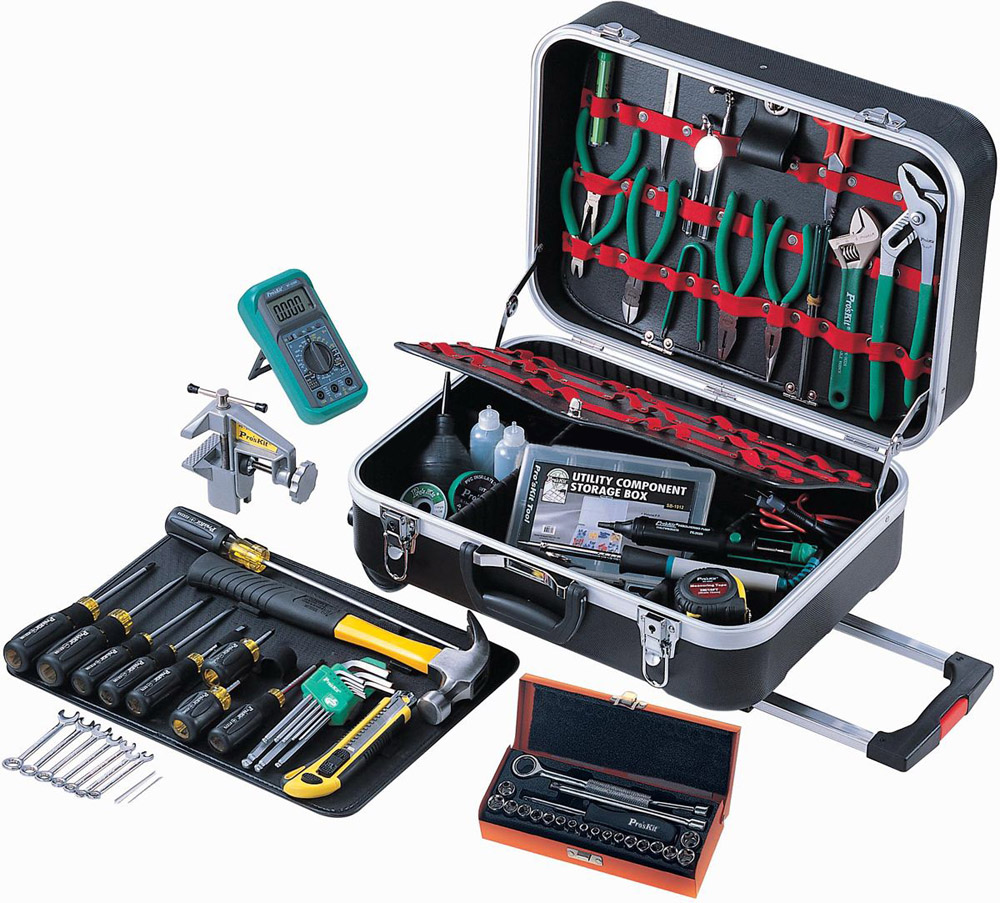
\includegraphics[height=0.95\textheight]{tech/tools/proskit/PK5308BM.jpg}

\textbf{PK-5308BM универсальный набор инструментов}

\clearpage
\noindent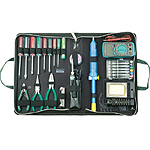
\includegraphics[height=0.95\textheight]{tech/tools/proskit/1PK-616B.jpg}

\textbf{1PK-616B Набор инструментов для электроники профессиональный}

\clearpage\label{1PK-813B}
\noindent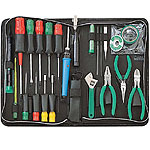
\includegraphics[height=0.95\textheight]{tech/tools/proskit/1PK-813B.jpg}

\textbf{1PK-813B Набор базовых инструментов для электроники}

\clearpage

По личному опыту: в 1PK-813B не хватает

\begin{itemize}
  \item мелкого мультиметра,
  \item стриппера 1PK-3001E,
  \item микрокусачек типа 8PK-30D,
  \item канифоли,
  \item ножа,
  \item настроечную отвертку заменить индикаторной.
\end{itemize}

\clearpage
\secrel{Инструмент до 1000\,В}

Для электромонтажных работ обязательно приобретите комплект
высоковольтного инструмента до 1000\,В:

\begin{tabular}{p{0.45\textwidth} p{0.45\textwidth}}
\noindent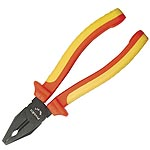
\includegraphics[width=0.45\textwidth]{tech/tools/proskit/PM-911.jpg}
&
\noindent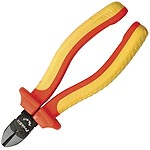
\includegraphics[width=0.35\textwidth]{tech/tools/proskit/PM-917.jpg}
\\

\textbf{PM-911 Пассатижи 1\,кВ}
&
\textbf{PM-917 Кусачки (бокорезы) 1\,кВ}
\\
\end{tabular}
\clearpage

\secrel{Хранение}

\begin{tabular}{p{0.45\textwidth} p{0.45\textwidth}}
\noindent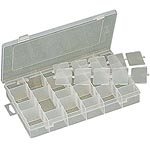
\includegraphics[width=0.45\textwidth]{tech/tools/proskit/103-132D.jpg}
&
\noindent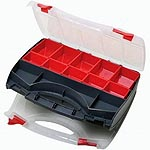
\includegraphics[width=0.45\textwidth]{tech/tools/proskit/SB-3428SB.jpg}
\\
\textbf{103-132D Кассетница для деталей и компонентов}
&
\textbf{SB-3428SB Портативная кассетница для саморезов и т.п.}
\\
\end{tabular}
\clearpage

\secrel{Радиомонтаж}

\begin{tabular}{p{0.45\textwidth} p{0.45\textwidth}}
\noindent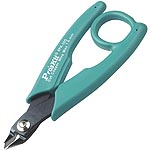
\includegraphics[width=0.45\textwidth]{tech/tools/proskit/8PK-30D.jpg}
&
\noindent\includegraphics[width=0.45\textwidth]{tech/tools/proskit/1PK-709.jpg}
\\
\textbf{8PK-30D Кусачки миниатюрные}
&
\textbf{1PK-709 Длинногубцы-кусачки}
\\
\end{tabular}
\clearpage

\begin{tabular}{p{0.45\textwidth} p{0.45\textwidth}}
\noindent\includegraphics[width=0.45\textwidth]{tech/tools/proskit/1PK-055S.jpg}
&
\noindent\includegraphics[width=0.45\textwidth]{tech/tools/proskit/1PK-29.jpg}
\\
\textbf{1PK-055S Длинногубцы изогнутые}
&
\textbf{1PK-29 Круглогубцы}
\\
\end{tabular}
\clearpage

\begin{tabular}{p{0.45\textwidth} p{0.45\textwidth}}
\noindent\includegraphics[width=0.45\textwidth]{tech/tools/proskit/1PK-101T.jpg}
&
\noindent\includegraphics[width=0.45\textwidth]{tech/tools/proskit/1PK-3001E.jpg}
\\
\textbf{1PK-101T Пинцет прямой}
&
\textbf{1PK-3001E Клещи для зачистки проводов прецизионные (стриппер)}
\\
\end{tabular}
\clearpage

\begin{tabular}{p{0.45\textwidth} p{0.45\textwidth}}
\noindent\includegraphics[width=0.45\textwidth]{tech/tools/proskit/PD-374.jpg}
&\\
\textbf{PD-374 Тиски на струбцине}
&\\
\end{tabular}
\clearpage

\secrel{Прочие}

Попалась интересная недорогая отвертка: aиксация четкая, исполнение очень
неплохое, позволяет добраться до узких мест. Из минусов: ручка похоже не
цельнометаллическая, при изломе есть риск распороть руку.

\bigskip
\noindent\includegraphics[width=0.4\textwidth]{tech/tools/P1020966.jpg}
\noindent\includegraphics[width=0.4\textwidth]{tech/tools/P1020967.jpg}
\clearpage

\secup




\section{Паяльное оборудование}

\subsection{Паяльник}

Паяльник\ --- обязателен дешевый сетевой мощностью не менее 20\,Вт, типа
ЭПСН-25/220. Ограничитель мощности или регулятор температуры легко собрать
самостоятельно.

Для сборки электроники хорошо также иметь маленький монтажный 12\,В 8\,Вт от
паяльной станции ZD-927 ($\sim$100\,р), без самой станции. Если не жалко 500\,р,
берите станцию ZD-927 целиком, внутри простейший регулятор мощности, и вам не
понадобится источник питания на 12\,В, который вы еще не сделали.

\noindent\includegraphics[width=0.4\textwidth]{tech/tools/solder/EPSN25.jpg}
\textbf{Паяльник ЭПСН-25/220}

\noindent\includegraphics[width=0.4\textwidth]{tech/tools/solder/SV-55310-25.jpg}
\textbf{Паяльник 220В 25Вт, СВЕТОЗАР, SV-55310-25 230\,р.}

\noindent\includegraphics[width=0.4\textwidth]{tech/tools/solder/ZD-721N.jpg}
\textbf{Паяльник 220В 25Вт ZD-721N 175\,р.}

\noindent\includegraphics[width=0.4\textwidth]{tech/tools/solder/Iron8W.jpg}
\textbf{Паяльник для станции ZD-927 12\,В 8\,Вт 85\,р.}

\subsection{Паяльная станция}

Из всего разнообразия для хоббита оптимальным являются паяльные станции Lukey
702/853D (3000+\,р). Для работы или регулярного хобби паяльная станция с феном,
а может даже и встроенным источником питания, вещь незаменимая, и не такая уж
дорогая.

\includegraphics[width=0.45\textwidth]{tech/tools/solder/ZD927.jpg}
\textbf{Паяльная станция ZD-927 520\,р.}

\includegraphics[width=0.45\textwidth]{tech/tools/solder/Lukey702.jpg}
\textbf{Паяльная станция LUKEY 702 3100\,р.}

\clearpage
\includegraphics[width=0.95\textwidth]{tech/tools/solder/Lukey853D.jpg}

\textbf{Паяльная станция LUKEY 853D с источником питания 5200\,р.}
\clearpage



% \section{JTAG-адаптер}
% 
% % \input{jtag/soft}
% % \input{stlink/stlink1}
% 
% \section{Отладочные платы}
% 
% Прежде чем начать работать с отдельными \mk, устанавливая их на плату
% собственной разработки, для быстрого старта используют \term{отладочные
% платы}\note{development board, demo board}
% 
% \subsection{Arduino /Atmel Mega AVR8/}
% 
% \subsection{Cortex-Mx} %См. \ref{devkitcmx}
% 
% \subsection{CubieBoard /Cortex-A8 AllWinner A10/}
% 
% \subsection{Raspberry Pi /ARM11 BCM3032/}
% 
% \subsection{BlackSwift /MIPS/}
% 
% \subsection{VoCore /MIPS/}

\secrel{Измерительное оборудование}\secdown

\secrel{Мультиметр}\label{mmetr}

\emph{Мультиметр\ --- обязателен, без него работать невозможно}\note{или
собирать замену на паре измерительных головок тока/напряжения, и делителях}.
Для совсем начинающего больше всего подойдет M320\ref{mmetr320} c
автодиапазоном, когда освоитесь возьмете вторым прибором что-то из крупных серий
M89x/MY6x с измерением температуры\note{иногда нужно для измерения температуры
корпусов элементов, радиаторов, растворов если возитесь с электрохимией}
или ``рыльцеметр''\ref{rlcmetr} (RLC).

\secdown
\secrel{Mastech M838}\label{mmetr838}

\begin{tabular}{p{0.3\textwidth} p{0.6\textwidth}}
\noindent\includegraphics[width=0.3\textwidth]{tech/tools/mes/M838.jpg}
&
Простой, компактный, дешевый, \emph{с измерением температуры}
\\
\end{tabular}

\secrel{Mastech M300}\label{mmetr300}

\begin{tabular}{p{0.3\textwidth} p{0.6\textwidth}}
\noindent\includegraphics[width=0.3\textwidth]{tech/tools/mes/M300.jpg}
&
Простой, \emph{очень компактный}, дешевый, в чехле очень удачно умещается в
набор инструментов.
\\
\end{tabular}

\secrel{Mastech M320}\label{mmetr320}

\begin{tabular}{p{0.3\textwidth} p{0.6\textwidth}}
\noindent\includegraphics[width=0.3\textwidth]{tech/tools/mes/M320.jpg}
&
То же что и M300\ref{mmetr300}, но с \emph{автодиапазоном}, т.е. не требует
переключения диапзонов измерения вручную. На любителя, возможно \emph{удобен для
совсем начинающих}, но слишком медленен если требуется измерение меняющегося
тока/напряжения.
\\
\end{tabular}

\secup

\secrel{Осциллограф}

\secrel{Логический анализатор}

\secrel{Генератор сигналов}

\secrel{Рыльцеметр RLC}\label{rlcmetr}

\secup

\secrel{Электроинструмент}\secdown

\secrel{Дрелъ}

% \noindent
% \begin{tabular}{p{0.5\textwidth} p{0.5\textwidth}}
% \noindent
% \includegraphics[width=0.45\textwidth]{tech/tools/PraktylR.jpg}
% &
% \noindent
% \includegraphics[width=0.45\textwidth]{tech/tools/D_11_530ER.jpg}
% \\
% \textbf{Дрель ударная сетевая} & \textbf{Дрель безударная сетевая} \\
% \textbf{Praktyl-R PID13D01 400\,Вт} 
% \href{http://leroymerlin.ru/catalogue/instrumenty/elektroinstrument/dreli\_udarnye/13805983/}{\textbf{(!)395\,р.}}
% &
% \textbf{Интерскол Д-11/530ЭР (с БЗП)}
% \href{http://leroymerlin.ru/catalogue/instrumenty/elektroinstrument/dreli\_bezudarnye/11857763/}{\textbf{1120\,р.}}
% \\
% \end{tabular}
% \bigskip
% 
% Дрель\ --- одноразовая китайчатина от 400\,р. Продаются уже брендированные на
% Леруа Мерлен, наклейка <<PID13D01 Ударная дрель 400\,Вт, 13\,мм>>. Скорость
% регулируется глубиной нажатия курка, крутилка на курке ограничивает глубину
% механически, фиксатор держит скорость близко к минимальной, запаха горелой
% пластмассы через несколько минут работы на холостом ходу нет.
% 
% По надежности рекомедуется Интерскол 1100+\,р. Надежность Интерскола\ --- не
% <<китай>>, классика ДУ-580ЭР работает в хвост и гриву, используется криворукими
% студентами, лежит в подвале в пыли от точила, и никаких вопросов даже со
% щетками.
% 
% Если не планируете много сверлить бетон, \textbf{берите дрель без ударного
% механизма}: отсутствуют лишние продольные перемещения, что может быть важно при
% использовании в качестве шпинделя сверлильного станка, и механизации других
% технологических поделок.
% 
% У шуруповерта нет 43\,мм шейки для фиксации, поэтому как средство электропривода
% он практически бесполезен, и нужен собственно для заворачивания большого
% количества саморезов. Хотя наличие ограничителя крутящего момента и малые
% габариты удобны при сверлении и сборке поделок.
% 
% \bigskip
% Имея некоторое количество поделочного материала, кривые руки и особенно доступ к
% станочному оборудованию, можно сколкозить некоторое подобие настольных
% станочков\ \pref{fig:drelstans}\ для механизации некоторых работ,
% используя дрель в качестве привода.
% 
% Главным элементом такой оснастки\ --- зажим на шейку дрели 43\,мм. Особых
% требований по его точности и качеству нет, т.к. сама шейка обычно пластиковая, и
% никакой доводки по круглости и параллельности оси инструмента не проходит.
% 
% \clearpage
% \phantomsection\label{fig:drelstans}
% \noindent\includegraphics[height=0.528\textheight]{tech/tools/DrelLathe.jpg}
% \noindent\includegraphics[height=0.528\textheight]{tech/tools/DrelShliph.jpg}
% 
% \noindent\includegraphics[height=0.465\textheight]{tech/tools/DrelLathe2.jpg}
% \noindent\includegraphics[height=0.465\textheight]{tech/tools/DrelBoren.jpg}
% \clearpage

\secrel{Лобзик}

% \noindent
% \begin{tabular}{p{0.5\textwidth} p{0.5\textwidth}}
% \noindent
% \includegraphics[width=0.45\textwidth]{tech/tools/LobzPraktyl.jpg}
% &
% \noindent
% \includegraphics[width=0.45\textwidth]{tech/tools/LobzMakita4329.jpg}
% \\
% \href{http://leroymerlin.ru/catalogue/instrumenty/elektroinstrument/lobziki/13805991/}{\textbf{Praktyl
% 350 Вт 356\,р.}} 
% & 
% \href{http://leroymerlin.ru/catalogue/instrumenty/elektroinstrument/lobziki/12114283/}{\textbf{Makita
% 4329 2260\,р.}}
% \\
% \end{tabular}
% \bigskip
% 
% Лобзик полезен при разделке стеклотекстолита, и изготовлении технологической
% мебели (стеллажи, рабочие столы и т.п.).

\secrel{Жвигатель}

% Если у вас возникло желание механизировать изготовление механических деталей, а
% свободного доступа к настоящему станочному оборудованию нет, есть смысл
% рассмотреть изготовление самодельной механизированной оснастки 
% типа\ \pref{fig:drelstans}, или даже самодельных станочков. В этом случае надо
% рассмотреть применения универсального привода.
% 
% Первый кандидат на место универсального электропривода достается той самой
% дрели, не забываем об обязательном наличии 43\,мм монтажной шейки.
% Достоинство дрели как привода\ --- прямое подключение к сети, встроенный
% редуктор, есть модели с простой регулировкой оборотов, есть резьба и отверстие
% под винт на валу, в комплекте есть патрон для зажима мелких деталей в
% точилке\footnote{\ БЗП удобен, патрон с ключем дает лучший зажим и возможно
% точнее}.
% 
% Ограниченно доставаемые двигатели от стиральных машин, отличаются мощностю и
% оборотистостью, особенно от старых моделей. Часто доступны сразу с готовым
% шкивом на валу, который иногда проще использовать, чем снять.
% 
% Автозапчасти: привод печки Камаза, двигатель постоянного тока 
% 24\,В 50\,Вт
% 
% Новые асинхронные двигатели АИРЕ 56 B2/B4 (3000/1500 об.) с заводским
% конденсатором, подключается к сети $\sim$220\,В, цена от 2500\,р.
% С ростом размеров и мощности цена резко повышается.
% Следует обратить внимание на возможность монтажа на дополнительный фланцевый
% подшипниковый щит, (?) с моделями АИРЕ 80.
% 
% Для самодельных серлилок и микроинструмента хороши китайские воздушные шпиндели
% постоянного тока с цанговыми патронами ER11. Требуют источник питания
% постоянного тока 9$\div$48\,В. В магазинах не попадались, необходима прямая
% покупка с \href{http://www.aliexpress.com/}{AliExpress}\note{пользуйтесь
% английской версией\ --- переводная жуткое УГ}\ по почте.
% 
% % \clearpage
% \begin{tabular}{l l}
% 
% \noindent\includegraphics[width=0.37\textwidth]{tech/tools/VyatkaDvig.jpg} 
% & 
% \noindent\includegraphics[width=0.37\textwidth]{tech/tools/KamazDvig.jpg}
% \\
% \textbf{Жвигатель Вятка-Автомат 19??\,г.}
% &
% \textbf{Двигатель печки Камаза}
% \\
% 
% \noindent\includegraphics[width=0.37\textwidth]{tech/tools/AIRE.jpg}
% & 
% \noindent\includegraphics[width=0.37\textwidth]{tech/tools/ER11.jpg}
% \\
% \textbf{АИРЕ 56 B2, 0.2\,КВт}
% &
% \textbf{Воздушный шпиндель с цангой ER11}
% \\
% 
% \end{tabular}
% \clearpage
% 
% Съемные фрезерные шпиндели, поставляются отдельно или в комплекте с насадкой
% ручного фрезера по дереву. Лучшие, со стальной шейкой\ --- Kress, активно
% применяются хобби-ЧПУшниками. Попроще и сильно дешевле делал Интерскол, иногда
% попадается noname. Недостаток как универсального привода\ --- они
% высокоскоростные, возникают проблемы с понижающими передачами. Применение\ ---
% приводной высокоскоростной инструмент: боры, фрезы по дереву, микроинструмент
% для граверов (микродиски, шарошки). Цанга 8\,мм. Для некоторых моделей бывают
% наборы цанг на мелкий инструмент.
% 
% \bigskip
% \begin{tabular}{p{0.3\textwidth} p{0.3\textwidth} p{0.3\textwidth} }
% \noindent\includegraphics[height=0.3\textheight,width=0.3\textwidth,keepaspectratio]{tech/tools/Kress530.jpg}
% &
% \noindent\includegraphics[height=0.3\textheight,width=0.3\textwidth,keepaspectratio]{tech/tools/Interskol30.jpg}
% &
% \noindent\includegraphics[height=0.3\textheight,width=0.3\textwidth,keepaspectratio]{tech/tools/InterskolFM55.jpg}
% \\
% KRESS 530/800/1050 FM(E)
% &
% Интерскол ФМ-30/750
% &
% Интерскол ФМ-55/1000 Э
% \\
% \href{http://kress-shop.ru/product/frezernyj-dvigatel-530-fm-kress-06082302/}{5600+\,р.}
% &
% /снят с производства/
% &
% \href{http://www.kuvalda.ru/catalog/1867/27920/}{5050\,р.}
% \\
% \end{tabular}

\secup



\secup


% % \secrel{Станки}\label{stanki}
\secdown

На основе \cp{http://rutracker.org/forum/viewtopic.php?t=3126529}

\copyright\ \prog{Joe Martin}, illustration by \prog{Craig Libuse}

\emph{Tabletop Machining}

A basic approach to making small parts on miniature machine tools

\bigskip

\copyright\ \prog{Джо Мартин}, иллюстрации \prog{Craig Libuse} 

\emph{Настольные станки}

Базовый подход к изготовлению мелких деталей на миниатюрных настольных станках

\clearpage
\secrel{A special note to engineers reading this book}

\secrel{Machining for engineen and engineering for machinists}

At first glance the subtitle on the cover of this book
could be a bit deceiving. What does tabletop
machining have do with engineering you may ask?
Compare it to a book that has been written about
the ocean. The seas could he described from the
perspective of a young man who has just sailed
around the world in a twenty-five foot sailboat or
by a merchant seaman who has spent his career
aboard a giant ocean liner. Each would have an
entirely different view of what the ocean was all
about. In a stenn, the chap in the small boat would
write ahout surviving broken masts and
mountainous seas while the merchant seaman might
write about seasick passengers. I believe you would
learn more ahout the ocean from the young man in
the small boat, because in a sense he was more
involved in his subject. He was not just on it, he
was in it.

\secrel{Navigating the seas of machining}

The ocean in this case is the world of machining.
The craftsman using tabletop machine tools is like
the sailor in a small boat, while the professional
machinist with his big CNC shop tools is like the
world-traveling seaman. The process of producing
complex, accurate parts cannot be described by
looking in the window of a quarter million dollar
CNC machine. It would be like a merchant seaman
working in the engine room trying to describe a
stonn in the Atlantic Ocean by telling you how much
extra fuel the ship used. The professional's view of
the subject may be so cluttered with details that it is
difficult to sort the things you really need to know
to sail in rough seas or make good parts. I t is the
craftsman working with small tools, turning the
cranks by hand, who will have the most to tell you
about the real world of working with metal.

\secrel{looking at engineering from the craftsman's perspedive}

With the aid of computers, parts can easily be drawn
that can't be built. CAD prvgrams allow a designer
to put a perfect .0001 " radius on the inside comer of
a pocket cut in tool steel. Hopefully after reading
this book you will not ask a toolmaker to do it, but
if you do, you'll at least know it is going to cost a
great deal of money to try. Working with metal is
far more difficult than one would imagine. A false
impression is gained by looking at the beautiful yet
inexpensive machined parts that we deal with daily.
They have been produced in very large quantities,
and that five-dollar part you may consider a "ripoff'
could easi ly cost five hundred dollars if you
had to manufacture just one. New engineers will
often think a toolmaker is a failure when the
seemingly simple part they design ends up costing
a thousand dollars to make. Most engineers wi ll
eventually have to deal with the craftsman who tum
their ideas into reality, and in reading this book I
would hope you come away with a new perspective
of what is really involved in producing a machined
part or a product. An alternate subtitle for the book
might have been "Things they should have taught
you in engineering school but didn't". This book
might be considered your textbook for a course
called "Reality WI".

\secrel{Seeing produdion from the point of view of both
the engineer and machinist}

My perspective on machining could be considered
unique because, in order to survive, I have had to
deal with every aspect of product design from
engineering to prototyping to tooling to
manufacturing to sales. In this book I have tried to
pass along the logic I used to solve the associated
problems. Understanding how a craftsman thinks
and works is an essential part of getting projects
done. Unless you are willing to build your designs
yourself, you are going to have to learn how to deal
with the craftsman who will actually build them.
The more you know about their methods.
personalities and unique problems, the better your
chances are for success. Smooth sailing.

\bigskip\copyright\ Joe Martin

\secrel{About the Joe Martin}

Joe Martin worked in the construction trades after graduating from high school,
but his real love was always building and fl ying radio controlled model
airplanes. When he decided to turn his hobby into a business and start his own
company making components for the radio control industry, he had to learn about
machining and toolmaking on his own. He simply couldn afford to hire anyone else
to set up the tools and make the molds. He has designed and taken to market
numerous products and owned several companies over the years. He began his
association with Sherline Products as an importer of Australi an-built lathes in
the early 1970's. Since then, Joe's company has grown to become the sole
manufacturer and worldwide distributor of Sherline machine tools.

Joe was one of the founders of the sport ofFonnula One model aircraft
competition as well as one of its early champions. His competitive nature seems
to find its way into whatever form of fun he pursues. He has been a winner in
sports from model airplane competition to ocean sai lboat racing and, most
recently, automobile racing.

Never one to be a spectator in life, he has tried and mastered many skills. In
this book, he passes on to you some of his hard-won knowledge about machining.
His down-to-earth s ty le is not hi gh ly polished. In fact, if you could say
that life has put a finish on him, it would probably be described as "" ground
or honed .. . ve ry company making components for the radio control industry, he
had to learn about machining and toolmaking on his own. He simply couldn afford
to hire anyone else to set up the tools and make the molds. He has designed and
taken to market numerous products and owned several companies over the years. He
began his association with Sherline Products as an importer of Australi an-built
lathes in the early 1970's. Since then, Joe's company has grown to become the
sole manufacturer and worldwide distributor of Sherline machine tools.
Joe was one of the founders of the sport ofFonnula One model aircraft
competition as well as one of its early champions. His competitive nature seems
to find its way into whatever form of fun he pursues. He has been a winner in
sports from model airplane competition to ocean sai lboat racing and, most
recently, automobile racing. Never one to be a spectator in life, he has tried
and mastered many skills. In this book, he passes on to acc urate but not slick.
I think his heartfe lt love of good too ls and miniature machining will be
apparent to all who read this book. Working with him these past 25 years is
certainly an experience I would not have wanted to miss.

\bigskip\copyright\ Craig Libuse

\secrel{Dedication}

\note{The photo COII/positioll ahol'e ix ajoillt effort. The photo a/Carl II'OS
taken by his wife Barbara. The photo o/Swall Lake. MOil/alia. a /m'odle spot oj
Carl's, was takeu byfrieud WaYl1e Arll/s/rOllg. The two images were composed ill
PIIO/OShopl by artist £Ioille lolli/IS}

Carl Hammons, my friend and business partner
for thirty years. died September 11 , 1997 as I
was writing this book. We shared thousands of
lunches and coffee breaks over the years we worked
together, and much of the knowledge I have passed
on in this book came from Carl. Carl and I shared
the rare distinction of having been partners not just
once, but twice. We both played different roles in
putting together the product line, and without him
it just isn't going to be as much fun.

When we joined forces for the second time. we had
an agreement that eliminated any need to financially
justify the purchase of a new piece of equipment.
We would buy machines that interested us and find
a job for them later. The laser engraver was a
perfect example of thi s, but now we couldn't get
along without it. It may seem contrary to smart
business practice, but that's the way we did it. I have
no regrets, for we were always the happiest when
we were confronted with a new set of technical
problems. Therefore. I dedicate this book to Carl
Hammons: my business partner, my friend.

\bigskip
I should also credit the English teachers in the
Cranston, Rhode Island school system for forcing a
not-so-willing student enrolled in the "boys general
class" to learn enough about our language to dare to
take on the task of expressing difficult concepts in
simple words. I graduated in 1953. You, the reader,
will be the ultimate judge of their (and my) success
in this undertaking.

\bigskip\copyright\ Joe Martin

\secrel{Safety Rules}
\secrel{Foreword}
\secrel{Introduction}
\secrel{A gallery of machining project photos}

\secrel{SECTION I-GENERAl MACHINING}
\secdown
\secrel{Craftsman Profile-Scotty Hewitt ........... 24}
\secrel{I. Getting information on machining. . . . . . 27}
\secrel{2. Do you need a lathe. a mill or bOlh? ........ 29}
\secrel{3. Materials for metalworking .............. 39}
\secrel{4. Processes for metalworking}
\secrel{4. I- Heat treating ............ ..• ...... 45}
\secrel{4.2-Metal fini shes ........... . ........ 46}
\secrel{4.3-Castings. . . ... .... ..... .... 49}
\secrel{4.4-----0ther ways 10 form metal .. .. .. . .. .. 5 1}
\secrel{4.5- Joining metal- Soldering}
\secrel{and we lding . . . . . . . .. . . .. . .. . 52}
\secrel{5. Using hand tools and abrasives .......... .. 57}
\secrel{6. Cutting tools for metalworking}
\secrel{6. I- General notes on cutting IDols . . 63}
\secrel{6.2- Cutting tools for both}
\secrel{the lathe and mill ................... 65}
\secrel{6.3-Lathe cutting tools ................. 72}
\secrel{6.4-Culter,S for milling ...... ....... .... 81}
\secrel{7. Measuring and measurement tools . . . 85}
\secrel{8. Cool ants and CUlling oils ................ 99}
\secrel{9. General machining terms . . .. . 101}
\secrel{10. Machine tool lubrication and maintenancc . 107}
\secup

\secrel{SECTION 2-LATHE OPERATIONS}
\secdown
\secrel{Craftsman Profile-Jerry Kieffer ..... .. .. .. . 112}
\secrel{Jerry Kieffer's Flying Pendulum Clock .. . .. 114}
\secrel{I. Lathe work holding ... .. . .. . .. .. .. . .. . . 115}
\secrel{2. Lathe operating instnlclions . . . . ......... 121}
\secrel{3. Tail slock lools and operations . . . . . ...... 141}
\secrel{4. Ri ser blocks .. . . . . . . . . . . . . ........... 145}
\secrel{5. Supporting long or thin work . . ... ... . . .. 149}
\secrel{6. Gelling started in thread cutting. . . . .. 157}
\secrel{7. Knurled fini shes. . . . . . . . .. .. . ....... 167}
\secrel{8. Watchmaking and clockmaking tools . ... . 171}
\secrel{9. Milling operations on a lathe . . . . .. . . . ... 177}
\secup

\secrel{SECTION 3-MIll1NG OPERATIONS}
\secdown
\secrel{Craftsman Profile- Augie Hiscano . ........ . 180}
\secrel{I. Holding parts for milling. . . . . . . . . . . . . 183}
\secrel{2. Mill operating in structions.. . . . ....... . 191}
\secrel{3. Squaring up a block ...... ........ .. .... 205}
\secrel{4. The rotary table and index ing attachment ..... 209}
\secrel{5. Gears and Geartrains ................... 2 19}
\secrel{6. Accessories for milling}
\secrel{• Horizontal milling conversion .... . ..... 235}
\secrel{• Rotary column attachmcnt . . . . . . .. 237}
\secup

\secrel{SECTION 4-OTHER MACHINING TOPICS}
\secdown
\secrel{Craft sman Profiles-Dan Lutz and Paul White . 242}
\secrel{I. Setting up a small workshop .... .... .... . 247}
\secrel{2. Lathe and mill alignment and adj ustments .. 25 1}
\secrel{3. Enginering drawings . .... .. ............ 259}
\secrel{4. Frequently asked questions . . . . .. . . . .. . . 265}
\secrel{5. Making a bus iness o ut of a hobby .. .Joe Martin's}
\secrel{and Sherline's story ................... 273}
\secrel{6. Using CNC in a home shop ... ........... 309}
\secup

\secrel{SECTION S-PROJECTS AND RESOURCES}
\secdown
\secrel{Cra ftsman Profi le-Bob Bres lauer ........... 3 16}
\secrel{Machini st's tips .......................... 3 18}
\secrel{I. Plans and projects you can build ........... 3 19}
\secrel{1. Miniature Tap Handle ... a beginning}
\secrel{project you can use in your shop ........... 32 1}
\secrel{2. Mill vise "sofe jaws. . . . . . . . . . . . . . . . 325}
\secrel{3. Lay ing out a circul ar hole pattern}
\secrel{fordrilling, a handy skill to learn. . .. . 327}
\secrel{4. "Millie" ... a small oscillating steam}
\secrel{engine by Ed Warren, a simple project}
\secrel{from the pages of Modeltec magazine) ..... . 329}
\secrel{5. Ordering plans for the Little Ange l}
\secrel{hit 'n miss engine ... an advanced}
\secrel{machining project by Bob Shores .......... 333}
\secrel{2. Contests and awards for tabletop machini sts . . 335}
\secrel{3. Exploded views and part number li sting}
\secrel{ Model 4000 and 4400 Lathes .. ......... 340}
\secrel{ Model 5000 and 5400 Milling machines . . . 341}
\secrel{ Model 2000 8-Direction Mill Column ..... 342}
\secrel{ Part number listing ... . ... . ........ . .. 343}
\secrel{4. A simple RPM gage for your latheor mill ... . 345}
\secrel{Harold Cli sby and the first Sherline lathe .... . 346}
\secrel{S. Index ............. .... ...... . . . 347}
\secrel{ Conversion faclors .. . ... . . .. .. ........ 350}
\secup

\secrel{Станочное оборудование}\secdown

Самый распространенные станки\ --- \term{сверлильные}, т.к. имеют самую простую
конструкцию, и минимальную стоимость. Предназначены для самой частой операции:
изготовления перпендикулярных круглых дырок в различных материалах, топовые
модели имеют также функцию нарезения резьбы.

\bigskip

Наиболее многочисленную группу металлорежущих станков составляют \term{токарные
станки}, используются в механических, инструментальных и ремонтных цехах
заводов, а также в ремонтных мастерских в основном для обработки деталей,
имеющих форму тел вращения. При использовании соответствующей оснастки позволяют
растачивать отверстия в призматических (прямоугольных) деталях, и фрезеровать
небольшие детали. Самый ходовой тип детали\ --- тело вращения с наружними и
внутренними резьбами: валики, втулки, оси, болты, винты, шпильки, кольца, шайбы
и т.д.

К основным размерам, характеризующим токарный станок, относятся 
\begin{itemize}
  \item наибольший допустимый диаметр обрабатываемой заготовки, 
  \item высота \term{центров} над станиной и 
  \item расстояние между центрами.
  \item 
Часто обращают внимание на диаметр \emph{проходного отверстия шпинделя},
определяющий максимальный диаметр \term{длинномерных заготовок}, что важно при
изготовлении мелких партий деталей или нарезке резьб на трубах.
\end{itemize}

\bigskip
Значительную часть среди металлорежущих станков составляют \term{фрезерные
станки}. Наибольшее распространение имеют консольно-фрезерные.
Предназначены для выполнения различных фрезерных работ цилиндрическими,
дисковыми, фасонными и другими \term{фрезами}, можно фрезеровать плоскости,
пазы, фасонные поверхности, и т.д. Кроме этого, универсальные
консольно-фрезерные станки c поворотным столом или делительной головкой
позволяют фрезеровать различного рода винтовые канавки и зубья зубчатых колес.

Основными размерами фрезерных станков, по которым можно определить возможность
установки и обработки конкретных заготовок с определенными габаритами, являются
размеры рабочей поверхности стола (длина и ширина) и \emph{рабочий ход
стола}/\term{рабочая зона} в продольном, поперечном и вертикальном направлениях.

\secrel{Маркировка моделей станков производства СССР}

\begin{tabular}{p{0.3\textwidth} p{0.6\textwidth}}
\includegraphics[height=0.3\textheight]{stanki/chugunok.jpg}
&
станок-''чугунок'', простой, дубовый, надежный (потому что ненадежные давно
сломались), дешевый, но требует помещение с силовым полом, 3х-фазное питание, и
кучу времени на поиск запчастей для восстановления по металлобазам и развалам. В
диком виде пока что встречается в школах и других типа учебных заведениях, т.к.
висит на балансе, но не эксплуатируется, и не обслуживается, потому что некем.
Отличается дешевизной (ржавого) инструмента и (еще более ржавой) оснастки, и
некоторым гемором с поиском запчастей.
\\
\end{tabular}
\clearpage


Для станков, выпускавшихся в СССР, принята единая система классификации и
условных обозначений, основанная на присвоении каждому станку особого шифра
(номера). Cтанки каждой группы подразделяются на девять \emph{типов}.
Внутри каждого типа металлорежущие станки могут отличаться друг от друга
конструктивными особенностями. Эти особенности, а также некоторые другие
характеристики и отражаются в шифре (номере) станка.

\begin{verbatim}
<группа>[<буква1>]<тип><характеризующий размер>[<буква2>]
\end{verbatim}

Кроме цифр, в условные обозначения модели станка часто входят буквы. Если
\emph{буква1} стоит между первой и второй цифрами, то это означает, что
конструкция станка подверглась усовершенствованию по сравнению с прежней
моделью. Если \emph{буква2} стоит в конце номера станка, то это говорит об
изменении основной, «базовой» модели станка.

\bigskip
\noindent\emph{группа}/\emph{тип}:
\begin{enumerate}[label={\arabic*}]
  \item токарные;
  \item сверлильные и расточные;
  \begin{enumerate}[label={\arabic*}]
    \item вертикально-сверлильные,
    \item одношпиндельные полуавтоматы,
    \item многошпиндельные полуавтоматы,
    \item координатно-расточные,
    \item радиально-сверлильные,
    \item горизонтально-расточные,
    \item алмазно-расточные,
    \item горизонтально-сверлильные,
    \item разные сверлильные.  
  \end{enumerate}
  \item шлифовальные, полировальные, доводочные и заточные;
  \item специальные;
  \item зубо- и резьбообрабатывающие;
  \item фрезерные;
  \item разрезные;
  \item строгальные, долбежные, протяжные;
  \item прочие
\end{enumerate}

\bigskip
\term{Характеризующий размер}:
\begin{description}
\item[токарные] \hfill \\
высота оси шпинделя над станиной, \\
задает \emph{максимально возможный радиус} обрабатываемой \emph{заготовки}
\end{description}


\clearpage
\section{\odina: станок токарно-винторезный}

\includegraphics[height=0.5\textheight]{stanki/1A616.jpg}

\subsection{Назначение и области применения}

\subsection{Распаковка и транспортировка}

\subsection{Фундамент станка, монтаж и установка}

\subsection{Подготовка станка к первоначальному пуску}

\subsection{Паспортные данные}

\subsection{Описание основных узлов}

\subsection{Смазка}

\subsection{Первоначальный пуск}

\subsection{Указания по технике безопасности}

\subsection{Настройка}

\subsection{Регулирование}

\subsection{Ведомость комплектации}

\secup

\secup

% % 
% % \secrel{Разработка ПО для встраиваемых систем}\secdown

% \chapter{Архитектура программных систем}

\section{Литература}

\cite{proghant}\ Программист-прагматик. Путь от подмастерья к мастеру
Хант Э., Томас Д., Лори/Питер, 2004, 2007

\section{Ортогональность}

\cp{http://ru.wikibooks.org/wiki/\%D0\%9E\%D1\%80\%D1\%82\%D0\%BE\%D0\%B3\%D0\%BE\%D0\%BD\%D0\%B0\%D0\%BB\%D1\%8C\%D0\%BD\%D0\%BE\%D1\%81\%D1\%82\%D1\%8C}

\term{Ортогональность}\ очень важна, если вы хотите создавать системы, которые
легко поддаются проектированию, сборке, тестированию и расширению. Однако этому
принципу редко обучают непосредственно. Часто он является лишь скрытым
достоинством других разнообразных методик, которые вы изучаете. Это неправильно.
Как только вы научитесь непосредственно применять принципы ортогональности, вы
сразу заметите, как улучшилось качество создаваемых вами систем.

\paragraph{Что такое ортогональность?}

Термин "ортогональность"\ заимствован из геометрии. Две линии являются
ортогональными, если они пересекаются под прямым углом, например, оси координат
на графике. В терминах векторной алгебры две \emph{такие линии перемещения
являются независимыми}. Если двигаться параллельно оси X вдоль одной из линий,
то проекция движущейся точки на другую линию не меняется. Этот термин был введен
в информатике для обозначения некой разновидности независимости или
несвязанности. В грамотно спроектированной системе программа базы данных будет
ортогональной к интерфейсу пользователя: вы можете менять интерфейс пользователя
без воздействия на базу данных и менять местами базы данных, не меняя
интерфейса. Перед тем как рассмотреть преимущества ортогональных систем,
познакомимся с неортогональной системой.

\paragraph{Неортогональная система}

Предположим, вы находитесь в экскурсионном вертолете, совершающем полет над
Гранд-Каньоном, когда пилот, который совершил ошибку, наевшись рыбы за обедом
внезапно вскрикивает и теряет сознание. По счастливой случайности это
происходит, когда вы парите на высоте 30 метров. Вы догадываетесь, что рычаг
управления общим шагом несущего винта обеспечивает подъем машины, так что, если
его слегка опустить, вертолет начнет плавно снижаться. Однако когда вы пытаетесь
сделать это, то осознаете, что жизнь\ --- не такая уж простая штука. Вертолет
клюет носом, и вас начинает вращать по спирали влево. Внезапно вы понимаете, что
управляете системой, в которой каждое воздействие имеет побочные эффекты. При
нажатии на левый рычаг вам придется сделать уравновешивающее движение назад
правым рычагом и нажать на правую педаль. Но при этом каждое из этих действий
вновь повлияет на все органы управления. Неожиданно вам приходится жонглировать
невероятно сложной системой, в которой любое изменение влияет на все остальные
управляющие воздействия. Вы испытываете феноменальную нагрузку: ваши руки и ноги
находятся в постоянном движении, пытаясь уравновесить все взаимодействующие
силы. Органы управления вертолетом определенно не являются ортогональными.

\paragraph{Преимущества ортогональности}

Как показывает пример с вертолетом, неортогональные системы сложнее изменять и
контролировать. Если составляющие системы отличаются высокой степенью
взаимозависимости, то невозможно устранить какую-либо неисправность лишь на
локальном уровне.

\bigskip
\emph{Исключайте взаимодействие между объектами, не относящимися друг к другу}
\bigskip

Мы хотим спроектировать компоненты, которые являются самодостаточным
независимыми, с единственным, четким назначением. Когда компоненты изолированы
друг от друга, вы уверены, что можно изменить один из них, не заботясь об
остальных. Пока внешние интерфейсы этого компонента остаются неизменными можете
быть спокойны, что не создадите проблем, которые распространятся по
\emph{всей}\ системе. С созданием ортогональных систем у вас появятся два
больших преимущества: увеличение производительности и снижение риска.

\paragraph{Увеличение производительности}

\begin{itemize}
\item Изменения в системе локализуются, поэтому периоды разработки и
тестирования сократятся. Легче написать относительно небольшие, самодостаточные
компоненты, чем один большой программный модуль. Простые компоненты могут быть
спроектированы, запрограммированы, протестированы и затем забыты\ --- не нужно
непрерывно менять существующий текст по мере того, как к нему добавляются новые
фрагменты.

\item Ортогональный подход также способствует многократному использованию
компонентов. Если компоненты имеют определенную, четкую сферу ответственности,
они могут комбинироваться с новыми компонентами способами, которые не
предполагались при их первоначальной реализации. Чем меньше связанность в
системах, тем легче их перенастроить и провести их обратное проектирование.

\item При комбинировании ортогональных компонентов происходит заметное
увеличение производительности. Предположим, что один компонент способен
осуществлять М, а второй\ --- N различных операций. Если эти компоненты
ортогональны и комбинируются, то в сумме они способны осуществить $M\times N$
различных операций. Но если два компонента не являются ортогональными, они будут
перекрываться, и результат их действия будет меньшим по сравнении с
ортогональными компонентами. Вы получаете большее количество функциональных
возможностей в пересчете на единичное усилие, если комбинирует между собой
ортогональные компоненты.
\end{itemize}

\paragraph{Снижение риска}

Ортогональный подход приводит к снижению уровня риска, присущего любой
разработке.

\begin{itemize}
\item Ошибочные фрагменты текста программы изолируются. Если модуль содержит
ошибку, то вероятность ее распространения на всю систему уменьшается. Кроме
того, ошибочный фрагмент может быть извлечен и заменен новым (исправленным).

\item Конечный продукт (система) становится менее хрупким. Проблемы,
появляющиеся при внесении небольших изменений и устранении недочетов на
определенном участке, не проходят дальше этого участка.

\item Ортогональная система способствует повышению качества тестирования,
поскольку облегчается проектирование и тестирование отдельных ее компонентов.

\item Вы не будете слишком сильно привязаны к определенному субподрядчику,
программному продукту или платформе, поскольку интерфейсы между компонентами,
производимыми фирмами-субподрядчиками, не будут играть главенствующей роли в
проекте.
\end{itemize}




\part{IDE}

IDE\ --- Integrated Development Environment, интегрированная среда разработки.

Программный пакет, включающий 
\begin{itemize}
  \item средства управления проектом,
  \item отслеживание зависимостей между файлами (в т.ч. с анализом исходного
  текста программ на конструкции типа \verb|#include|, \verb|module|,
  \verb|uses|),
  \item автозапуском компиляторов для изменившихся файлов,
  \item GUI для отладчиков (gdb),
  \item специализированный редактор plain text\note{файлы не включающие
  непечатаемых символов и бинарных данных, которые можно причитать простым
  выводом на экран командами типа \textbf{type}, \textbf{cat}, \textbf{more}}
  файлов c
  \begin{itemize}
    \item цветовой и шрифтовой \term{подстветкой синтаксиса},
  	\item \term{автодополнением}: дописываются имена объектов программ, 
  	синтаксические конструкции и параметры функций,
 \item \term{автоформатированием}: фрагмент текста переформатируется в
 соответствии с синтаксисом языка редактируемого файла, проставляются отступы в
 зависимости от вложенности синтаксических конструкций типа циклов и условных
 блоков)
  	\item выделением строк, на которые указывают сообщения об ошибках
  	компиляторов,
  	\item маркеры точек останова отладчика
  \end{itemize}
  \item отображение структуры программ, например деревья классов и структур
  данных
  \item контекстные справочники по используемым языкам программирования,
  автоматический вывод списка параметров при вводе имени функции
  \item отображение дизассемблерных листингов для компилируемых языков
  \item отображение браузера как вкладки или MDI окна
  \item отображение вывода \term{статических анализаторов} программ c
  кликабельными ссылками
  \item вывод компиляторов и трансляторов с цветовым выделением и переход на
  ошибочную строку в редакторе при щелчке на ошибке
  \item \ldots
\end{itemize}

В этой книге рассмотрены три бесплатных мультиплатформенных OpenSource IDE, в
порядке навороченности, универсальности, и требуемым ресурсам для работы самой
среды:

\begin{enumerate}
  \item \eclipse\ \ref{eclipse}: самая навороченная и ресурсоемкая IDE, написана
  на Java, имеет десятки дополнительных модулей на все случаи, умеет работать со
  всеми распространенными языками программирования, жрет память, и требует
  современного компьютера минимум с 2+ Гб ОЗУ. Последний релиз \eclipse\ Luna
  работает заметно быстрее (особенно при запуске). 
  \item Code::Blocks \ref{cb}: легкая среда для разработки на C/\cpp, для других
  языков модет потребоваться написать свои модули или файлы описания синтаксиса
  \item \vim\ \ref{vim}: самый легкий и \emph{портабельный} универсальный
  текстовый редактор с расширенными функциями, работает на всех
  существующих платформах (кроме совсем уж embedded), использует минимум
  ресурсов, но требует некоторого обучения даже чтобы выйти из \verb|vim|
  \smiley
\end{enumerate}

\secrel{\eclipse}\label{eclipse}\secdown

\includegraphics[height=0.5\textheight]{logo/eclipse.png}

\secrel{Установка \eclipse\ под \win}

\menu{\winr>\url{https://eclipse.org/}>Download>Eclipse Luna release for>\win}

Качаем архив базовой системы:
\menu{Eclipse IDE for Java Developers>\win\ 32/64 Bit}

Или сразу сборку CDT\eclipse:
\menu{Eclipse IDE for C/C++ Developers>\win\ 32/64 Bit}

\secrel{Установка \eclipse\ под \linux}

\menu{\winr>\url{https://eclipse.org/}>Download>Eclipse Luna release for>\linux}

Качаем архив базовой системы:
\menu{Eclipse IDE for Java Developers>\linux\ 32/64 Bit}

Или сразу сборку CDT\eclipse:
\menu{Eclipse IDE for C/C++ Developers>\linux\ 32/64 Bit}

\bigskip

Пока качается, параллельно устанавливаем в систему Java-рантайм:

\begin{verbatim}
sudo aptitude install openjdk-7-jre
\end{verbatim}

Распаковывем полученный архив
\file{eclipse-java-luna-SR1-linux-gtk-x86\_64.tar.gz}
в \file{\$HOME}:

\begin{verbatim}
cd ~
tar zx < Downloads/eclipse-java-luna-SR1-linux-gtk-x86_64.tar.gz
ls -la eclipse/eclipse
-rwxr-xr-x 1 user user 74675 Авг 13 16:12 eclipse/eclipse
\end{verbatim}

Прописываем запуск \eclipse\ в ваш оконный менеджер или \file{.blackboxmenu}
с параметром \file{-noSplash} для лечения глюка с запуском на x64-битных
системах:

\lst{.blackbox.menu}{}{ide/eclipse_blackbox.menu}

\secrel{Установка CDT}

\href{https://eclipse.org/cdt/}{\prog{CDT}}\ --- расширение \eclipse\ для
разработки на Си/\cpp, редактирования make-файлов. Это расширение критически
важно для вашей работы, поэтому ставить его обязательно, или сразу качать сборку
CDT\eclipse.
\bigskip

\menu{\eclipse>Help>Install New Software\ldots}

\menu{Work with>Add>Add repository}

\menu{Name>CDT}

\menu{Location>\url{http://download.eclipse.org/tools/cdt/releases/8.5}}

\menu{OK}

\menu{Work with>CDT}

\menu{CDT Main Features>\checkbox\ C/C++ Development Tools}

\menu{CDT Optional Features}

Парсер файлов исходников на диалекте С99:
\menu{\checkbox\ C99 LR Parser}

Поддержка \prog{gcc}\ в режиме кросс-компиляции:
\menu{\checkbox\ GCC Cross Compiler Support}

Аппаратная отладка через \prog{gdb}:
\menu{\checkbox\ GDB Hardware Debugging}

\menu{Next>Next>Accept>Finish}

\secrel{Установка PyDev}

\href{http://pydev.org/}{\prog{PyDev}}\ --- расширение для разработки на Python:
\bigskip

\menu{\eclipse>Help>Install New Software\ldots}

\menu{Work with>Add>Add repository}

\menu{Name>PyDev}

\menu{Location>\url{http://pydev.org/updates}}

\menu{OK}

\menu{Work with>PyDev}

\menu{PyDev>\checkbox\ PyDev for Eclipse}

\menu{Next>Next>Accept>Finish>Certitificate>Restart Eclipse>Ok}

\secrel{Установка TeXlipse}

Если планируете работать с документацией в формате \LaTeX, установите расширение
\href{http://texlipse.sourceforge.net/}{\prog{TeXlipse}}:
\bigskip

\menu{\eclipse>Help>Install New Software\ldots}

\menu{Work with>Add>Add repository}

\menu{Name>TeXlipse}

\menu{Location>\url{http://texlipse.sourceforge.net/}}

\menu{OK}

\menu{Work with>TeXlipse}

Это расширение поддерживает подсветку синтаксиса, автодополнение, построение
динамического оглавления, автокомпиляцию по сохранению, и несколько визардов
создания проекта.

\secrel{Редактирование файлов в формате XML и производных}

Установите пакет \eclipse\ WST:

\menu{Help>Install New Software}

\menu{Work with:>Luna - http://download.eclipse.org/releases/luna}

\menu{Filter:>WST>Eclipse WST>Next>Next>Restart>OK}

\secrel{Проверка орфографии}

\cp{http://www.simplecoding.org/proverka-orfografii-v-eclipse.html}

То, что проверка орфографии очень удобная вещь вряд ли нужно объяснять. Есть
конечно люди, которые не обращают на неё внимание, но это чаще всего из-за
экономии времени и отсутствия удобных средств проверки.

Действительно, удобная автоматическая проверка орфографии есть в офисных
пакетах, но мне сложно представить разработчика, который будет переносить
комментарии в Word и обратно \smiley.

Поэтому очень удобно иметь \emph{проверку правописания прямо в IDE}. И \eclipse\
в этом смысле полностью соответствует ожиданиям.

Долго объяснять что к чему нет смысла. Проверка орфографии встроена в \eclipse\
и если вы пишите только на английском, то может быть не захотите ничего менять.

Кроме того, есть
\href{http://www.102degrees.com/blog/2007/07/09/spell-checking-in-eclipse-pdt/}{статья
Aaron'а} (en) в которой автор рассказывает о подключении дополнительных словарей
и плагине \file{eSpell}.

Но \emph{русских словарей в дистрибутиве нет}, а при подключении внешних есть
нюансы. Поэтому мы максимально подробно рассмотрим \emph{подготовку и добавление
русских словарей}.

Первый вопрос. В каком виде должны быть словари и где их взять?

Тут всё просто. Формат словаря\ --- обычный текстовый файл, в котором каждое
слово начинается с новой строки. И нам вполне подойдут свободно распространяемые
словари \file{aSpell}.

Установка состоит из \ref{aspellecl}\ шагов:
\begin{enumerate}
  \item качаем \href{}{aSpell}\ и словари для нужных языков

  \menu{\winr>\url{http://aspell.net/win32/}>}

  \menu{Binaries>Full installer}

  \menu{Precompiled dictionaries>English}

  \menu{Precompiled dictionaries>Russian}

  \item устанавливаем сначала \file{aSpell}, потом отдельно каждый словарь

  \menu{\file{Aspell-0-50-3-3-Setup.exe}>Setup GNU Aspell>Next>License>Next}

  \menu{Directory>\file{C:/GnuWin32/Aspell}>Next>Next}

  \menu{Additional>Next>Install>Next>\uncheckbox\ View manual>Finish}

  \menu{\file{Aspell-en-0.50-2-3.exe}>Aspell English Dictionary>Next>License>Next}

  \menu{Directory>\file{C:/GnuWin32/Aspell}>Next>Next>Install>Finish}

  \menu{\file{Aspell-ru-0.50-2-3.exe}>Aspell Russian Dictionary>Next>License>Next}

  \menu{Directory>\file{C:/GnuWin32/Aspell}>Next>Next>Install>Finish}

  \item делаем дамп словарей, перекодируем из koi8r в utf8 и объединяем

  \menu{\winr cmd}

\begin{lstlisting}
cd \GnuWin32\Aspell
bin\aspell dump master en > en.dict
bin\aspell dump master ru > ru.koi8
iconv -f koi8-r -t utf-8 < ru.koi8 > ru.dict
copy en.dict + ru.dict enru.dict
\end{lstlisting}

  \item \label{aspellecl} настраиваем \emph{spell-checker} \eclipse

  \menu{\eclipse>Window>Preferences>Editors>Text editors>Spelling}

  \menu{User defined dictionary>\file{C:/GnuWin32/Aspell/enru.dict}}

  \menu{Encoding>UTF-8}

  \menu{Apply>OK}

\end{enumerate}

\secup

\secrel{\cb}\label{cb}\secdown
\secup

\chapter{\vim}\label{vim}

\includegraphics[width=0.3\textwidth]{logo/vim.png}

\section{Установка под \win}

\menu{\winr cmd > \url{http://www.vim.org/} > Download > PC: MS-DOS and
MS-Windows > \href{ftp://ftp.vim.org/pub/vim/pc/gvim74.exe}{\file{gvim74.exe}}}

\menu{Vim 7.4 Setup>This will install>Да}

\menu{License>I'm Angry}

\menu{Installation Options>\checkbox\ Create .bat files>Next}

\menu{Installation Folder>Install}

\menu{Completed>Close}

\menu{Do you want to see README>\textbf{Да}}
\bigskip

Теперь можно настроить темную тему и выключение подстветки синтаксиса, по
умолчанию после установки используется светлая тема и подстветка выключена:

\nopagebreak
\menu{меню>Правка>Настройка запуска}
\bigskip

Переходим в конец файла и включаем \emph{режим вставки}

\keys{Ctrl+Down}\ \keys{Ins}\ \keys{Enter}\keys{Enter}

\begin{lstlisting}
syntax on
colorscheme pablo
\end{lstlisting}
\bigskip

Выходим в \emph{режим команд} и принудительно сохраняем

\keys{Esc}:\keys{w}\keys{!}\keys{Enter}\keys{Enter}
\bigskip

\textbf{Выходим из \vim}

\keys{Esc}:\keys{q}\keys{!}\keys{Enter}

\bigskip
Если не получилось (под Windows 7):

\bigskip
\menu{\winr cmd > \file{/Program Files (x86)/Vim/}}
\bigskip

Копируем файл \file{\_vimrc}\ в любой каталог, например в \file{/tmp/},
затем \menu{\rms\rms>Edit with Vim}, и повторяем редактирование еще раз.

\bigskip
Затем копируем \file{\_vimrc}\ обратно в \file{/Program Files (x86)/Vim/}\ с
заменой.

\bigskip
Если теперь открыть на редактирование тот же файл, или любой другой текстовый,
получим более удобный вид: для файлов известных типов будет работать подсветка
синтаксиса.

\nopagebreak\bigskip
\includegraphics[height=0.9\textheight]{ide/vim28.png}

\section{Выход из \vim}

\keys{Esc}\ :\ \keys{!}\ \keys{q}\ \keys{Enter}

\subsection{Выход с автосохранением}

\keys{Esc}\ \keys{Shift+Z}\ \keys{Shift+Z}

\section{Переход в режим редактирования}

\vim\ запускается в \emph{командном режиме}, для перехода в режим редактирования
используются следующие клавиатурные команды:

\begin{itemize}
  \item \keys{Ins}\ или \keys{i}: включение \emph{режима вставки} по текущему
  положению курсора
  \item \keys{Ins}\keys{Ins}\ или \keys{r}: включение \emph{режима перезаписи}
  поверх текста после курсора
  \item \keys{Shift+A}: включение режима вставки \emph{в конец текущей строки}
\end{itemize}

\section{Переход в режим команд}

\keys{Esc}

\section{Запись редактируемого файла}

\keys{Esc}\ :\ \keys{w}\ \keys{Enter}
\bigskip

Если выводится предупреждение типа ``файл защищен от записи'' или подобное,
может сработать принудительная запись:

\bigskip
\keys{Esc}\ :\ \keys{!}\ \keys{w}\ \keys{Enter}

\section{Перезагрузка файла}

Для перезагрузки возможно изменененного извне файла или отмены всех
несохраненных изменений

\bigskip
\keys{Esc}\ :\ \keys{e}\ \keys{Enter}

\section{Отмена последних изменений (undo)}

\keys{Esc}\keys{u}\keys{u}\ldots



\secrel{\prog{Make}: управление сборкой проектов}\label{make}

\secrel{VCS: cистемы контроля версий}\label{vcs}\secdown

\secrel{CVS}

\secrel{Subversion}

\secrel{Git}
\secdown

\secrel{GitHub}

\secup

\secup


\chapter{Вспомогательные скрипты на языке \py}

\begin{tabular}{p{0.1\textwidth} p{0.8\textwidth}}
\includegraphics[width=0.1\textwidth]{python/logo.png}&
\emph{
Название языка произошло вовсе не от вида пресмыкающихся. Автор назвал язык в
честь популярного британского комедийного телешоу 1970-х «Летающий цирк Монти
Пайтона». Впрочем, всё равно название языка чаще ассоциируют именно со змеёй,
нежели с передачей\ --- пиктограммы файлов в KDE или в Microsoft Windows и даже
эмблема на сайте \url{http://www.python.org} (до выхода версии 2.5) изображают
змеиные головы.
}
\\
\end{tabular}
\bigskip

\py\note{в оригинале читается \textbf{п\'{а}йтон}, но давно русифицировался как
\textbf{пит\'{о}н}}\ --- высокоуровневый язык программирования общего
назначения, ориентированный на повышение производительности разработчика и
читаемости кода.

\py\ удобно применять для написания различных вспомогательных скриптов.
Часто его используют при разработке сложных программных систем для написания
первых версий. В процессе работы над большими программами часто перерабатываются
большие объемы кода, поэтому для ускорения разработки требуется максимально
высокоуровневый язык. После того как архитектура программы стабилизируется,
узким местом становится производительность, и программу переписывают на более
низкоуровневом компилируемом языке, чаще всего \cpp.

Написание программ упрощают:

\begin{itemize}
  \item \textbf{объектно-ориентированное программирование} облегчает разработку
  программ, позволяет переопределить стандартные операторы для пользовательских
  типов данных, упрощая синтаксис
  \item \textbf{динамическая типизация} не требуется заранее упределять
  переменные, они создаются простым присваиванием
  \item \textbf{обработка исключений} для секции кода можно определить
  обработчик ошибок
  \item \textbf{высокоуровневые структуры данных}\ --- списки, словари (набор
  элементов ключ:значение), очереди
  \item богатая стандартная библиотека и множество дополнительных библиотек на
  все случаи
\end{itemize}

\section{Установка под \win}\label{pywinstall}

\bigskip
\menu{
\keys{\winstart+R}
>
\url{http://www.python.org}
>
Downloads
>
\href{https://www.python.org/ftp/python/2.7.8/python-2.7.8.msi}{Python 2.7.8}
}

\bigskip
\menu{\file{python-2.7.8.msi}
>
Setup>
for all users/for me
}

\menu{Destination Directory > \file{C:/Python/} > Next}

\nopagebreak
\bigskip
\includegraphics[width=0.45\textwidth]{python/install/037.png}
\includegraphics[width=0.45\textwidth]{python/install/038.png}
\bigskip


\menu{Customize > Python > Add python.exe to PATH > Next > Finish}

\nopagebreak
\bigskip
\includegraphics[width=0.45\textwidth]{python/install/039.png}
\includegraphics[width=0.45\textwidth]{python/install/045.png}
\bigskip

\section{Дополнительные материалы}

\cite{pyotkidach} Г. Россум, Ф.Л.Дж. Дрейк, Д.С. Откидач, 
\href{http://rus-linux.net/MyLDP/BOOKS/python.pdf}{Язык программирования Python}

\cite{pythink} Аллен Дауни
\href{https://drive.google.com/file/d/0B0u4WeMjO894Q2hWV1QwOFFQOVk/view?usp=sharing}{Думать
на языке \py: Думать как компьютерный специалист}



\secrel{Основы Си и \cpp}\secdown
\secup


\secrel{Лексический и синтаксический анализ}\secdown

Очень часто в практике возникает необходимость работы с данными в текстовых
форматах\ --- \termdef{plain text}{plain text} файлы, в которых в каком-либо
формате (на языке разметки, или \termdef{DDL}{DDL}: \termdef{[D]ata
[D]efinition [L]anguage}{Data Definition Language}) описаны данные. И от вас
требуется реализовать разбор такого файла, выделяя синтаксические структуры и
элементы данных, чтобы в дальнейшем после их преобразования например записать
текстовый файл в другом формате.

В таком виде хранятся результаты расчетных программ, работащих в пакетном
режиме, данные с измерительных систем, поток данных с приемников
GPS\note{протокол NMEA 0183}, очень популярный мета-формат XML со всеми его
частными случаями типа HTML, XLIFF\ref{xliff}, OpenDocument, тексты программ
для станков с ЧПУ,\ldots

С некоторыми хинтами точно так же можно работать и с бинарными файлами,
преобразовав их сначала в текстовую форму (в простейшем случае просто сделав hex
dump).

В некоторых случаях необходимо написание трансляторов форматов (текстовых)
данных, или даже интерпретаторов/компиляторов языков программирования.

\bigskip
Все эти техники с использованием стандартных утилит \prog{flex}\ и \prog{bison}\
будут кратко описаны в этой главе. Подробнее эти техники рассмотрены в
книгах\ref{lexlit}, особенно стоит отметить талмуд
\textbf{DragonBook}:

\bigskip

\label{exdragon}\cite{dragonbook} \textbf{Книга Дракона}: Ахо, Сети, Ульман
Принципы построения компиляторов.

\bigskip

\href{http://habrahabr.ru/post/99162/}{Habr: Компиляция. 1: лексер}

\href{http://habrahabr.ru/post/99298/}{Habr: Компиляция. 2: грамматики}

\href{http://habrahabr.ru/post/99366/}{Habr: Компиляция. 3: бизон}

\href{http://habrahabr.ru/post/99397/}{Habr: Компиляция. 4: игрушечный ЯП}

\href{http://habrahabr.ru/post/99466/}{Habr: Компиляция. 5: нисходящий разбор}

\href{http://habrahabr.ru/post/102597/}{Habr: Компиляция. $5\frac{1}{2}$: llvm
как back-end}

\href{http://habrahabr.ru/post/99592/}{Habr: Компиляция. 6: промежуточный код}

\bigskip

\url{http://ds9a.nl/lex-yacc/cvs/lex-yacc-howto.html}

\url{http://alumni.cs.ucr.edu/~lgao/teaching/flex.html}

\url{http://www.capsl.udel.edu/courses/cpeg421/2012/slides/Tutorial-Flex\_Bison.pdf}

\secrel{Лексер и лексический анализ, утилита \prog{flex}}

\begin{framed}
\noindent
\termdef{Л\'{е}ксер}{лексер}/\termdef{сканер}{сканер}\ --- программа или ее
часть, которая \begin{enumerate}[nosep]
  \item
получает на вход исходные
данные в виде сплошного потока одиночных сиволов,
  \item
группирует символы согласно
набору правил (заданных \termdef{регулярными выражениями}{регулярное
выражение}) и
  \item
отдает на выходе символы, уже сгруппированные в \termdef{лекс\'{е}мы}{лексема}\
или \termdef{ток\'{е}ны}{токен}.
\end{enumerate}
Цель лексера\ --- подготовить последовательность лексем для входа другой
программы. \\
В самый простых случаях на лексер можно возложить простые преобразования текста.
\end{framed}

\termdef{Лексический анализ}{лексический анализ}\ --- процесс программного
разбора входной последовательности символов\note{например, такой как исходный
код на одном из языков программирования} с целью получения на выходе
последовательности групп символов\ --- \term{токенов}, имеющих собственное
смысловое значение\note{подобно группировке букв в слово}. Как правило,
лексический анализ производится в соответствии набора правил определённого
\term{формального, искуственного или компьютерного языка}.

\begin{framed}\noindent
\term{Компьютерный язык}, а точнее его \termdef{грамматика}{грамматика}, задаёт
определённый набор лексем, которые могут встретиться на входе лексера, и набор
правил, по которым их следует группировать.
\end{framed}

Традиционно принято организовывать процесс лексического анализа, рассматривая
входную последовательность символов как поток одиночных символов. При такой
организации \term{лексер}\ самостоятельно управляет выборкой отдельных символов
из входного потока.

Распознавание лексем с учетом грамматики обычно производится путём их
идентификации согласно идентификаторам токенов, определяемых грамматикой языка.
При этом любая последовательность символов входного потока (лекс\'{е}ма),
которая согласно грамматике не может быть идентифицирована как токен языка,
обычно рассматривается как специальный \term{токен-ошибка}.

\bigskip
Каждый выделенный токен можно представить в виде парной структуры,
содержащей
\begin{enumerate}
  \item идентификатор токена и
  \item саму последовательность символов лексемы, выделенной из входного
потока\note{запись строки, числа и т. д.}.
\end{enumerate}

\bigskip
Рассморим обработку текстового файла: разделение текстового фрагмента на абзацы,
запись в формате
\href{http://docs.oasis-open.org/xliff/xliff-core/xliff-core.html}{XLIFF} для
перевода в системе \href{http://smartcat.pro}{ABBYY SmartCAT}, и обратной
трансляции из XLIFF в \LaTeX-совместимое форматирование.

\bigskip
Так как задача построения \termdef{лексических анализаторов}{лексический
анализатор} является стандартной задачей информатики, был разработан типовой
инструмент: \term{генератор лексических анализаторов} \prog{flex}. Эта программа
транслирует описание лексера на своем высококоуровневом языке в фрагмент
программы на языке Си/\cpp\ или самостоятельную программу. Описание лексера
прописывается в \file{.lex}-файле в формате:

\begin{verbatim}
определения, опции, декларации
%%
правила выделения токенов через регулярки
%%
сишный код
\end{verbatim}

\paragraph{Комментарии} поддерживаются сишные \verb|/* */| комментарии.

\paragraph{Опции} \verb|%option|

\bigskip\noindent
\begin{tabular}{l l}
noyywrap & отключает вызов лексером функции \verb|yywrap()| при достижении
конца текущего файла \\
main & включение типовой функции \verb|main()| вместо заданной пользователем \\
case-insensitive & регистро-независимый лексический анализ, большие/маленькие
буквы не различаются \\
yylineno & в глобальной си-переменной \verb|yylineno| доступен номер
текущей строки \\
\end{tabular}

\paragraph{Формат опреления} \verb|имя определение|:
\begin{verbatim}
digit    [0-9]
number   [\+\-]{0,1}{digit}+\.{digit}*
\end{verbatim}

\paragraph{Декларации на Си} прописываются в скобках \verb|%{ }%|

\cp{http://matt.might.net/articles/standalone-lexers-with-lex/}

\lstx{Makefile}{}{xliff/Makefile}{mk}

\lst{\prog{flex} лексер}{}{xliff/tex2xliff.l}

\secrel{Генератор синтаксических анализаторов \prog{bison}}

\begin{framed}\noindent
\termdef{Синтаксический анализ}{синтаксический анализ}\ --- процесс анализа
последовательности токенов с определением их грамматической структуры. На этом
этапе выделяются \term{синтаксичекие ошибки}.
\end{framed}

\lst{\prog{bison} парсер}{}{xliff/tex2xliff.y}

%\lst{\file{X.tex}}{}{xliff/X.tex}

%\lst{\file{xliff.xliff}}{}{xliff/xliff.xliff}

\secup


\secup

% % 
% % \secrel{Микроконтроллеры \cmx}
\secdown

\secrel{Производители}\secdown
\secrel{ST Microelectronix STM32}\secdown
\secup

\secrel{LPC}\secdown
\secup

\secrel{Миландр}\secdown
\secup

\secup


\secrel{Отладочные платы}\secdown

\secrel{LeafLabs Maple Mini: STM32F103 /\cm{3}/}
\secdown
\secup


\secrel{Серия STM32 STM32DISCOVERY}\secdown
\secrel{STM32DISCOVERY: STM32F103 /\cm{3}/}

\secrel{STM32F4DISCOVERY: STM32F406 /\cm{4F}/}

\secrel{STM32F0DISCOVERY: STM32F040 /\cm{0}/}

\secup

\secup

% \label{devkitcmx}
% 
% \secdown
% 
% \secrel{STM32DISCOVERY /\cm{3} STM32F103/}
% 
% \secrel{STM32F4DISCOVERY /\cm{4} STM32F407/}
% 
% \secrel{Maple Mini /\cm{3} STM32F100/}
% 
% \secup

\secup


\part{Встраиваемый \emlinux}

Linux для встраиваемых систем\note{будем называть его
\termdef{em\linux}{em\linux}}\ --- популярный метод быстрого создания комплекса
ПО для больших сложных приложений, работающих на достаточно мощном железе,
особенно предполагающих интенсивное использование сетевых технологий.

За счет использования уже существующей и очень большой базы исходных текстов
ядра, библиотек и программ для \linux, бесплатно доступных в т.ч. и для
коммерческих приложений, можно на порядки сократить стоимость разработки
собственных программных компонентов, и при этом получить готовую команду
бесплатных стронних разработчиков, уже знакомых с созданием ПО для \linux.

Из недостатков можно отметить:
\begin{itemize}
  \item Отсутствие полноценной поддержки режима жесткого реального времени;
  \item Тяжелое ядро;
  \begin{itemize}
  \item Поддерживаются только мощные семейства процессоров\note{32-бит,
  необходим блок MMU};
  \item Значительные требования по объему \ram\ и общей производительности;
  \end{itemize}
  \item Дремучесть техспециалистов, контуженных ТурбоПаскалем и
Win\-dows\-ом;
\end{itemize}

Для \termdef{сборки}{сборка}\ em\linux-системы используется метод
\termdef{кросс-компиляции}{кросс-компиляция}, когда используется
\termdef{кросс-тулчейн}{кросс-тулчейн}, компилирующий весь комплект ПО для
компьютера с другой архитектурой. Типичный пример\ --- сборка ПО на ПК c
процессором Intel i7 для Raspberry Pi или планшета на процессоре
AllWinner/Tegra/\ldots.

em\linux\ очень широко применяется на рынке мобильных устройств\note{в т.ч.
является основой Android}, и устройств интенсивно использующих сетевые протоколы
(роутеры, медиацентры).

В качествe примера применения рассмотрим относительно простое приложение:
многофункциональные настенные часы с синхронизацией времени через \internet, с
будильником, медиапроигрывателем, блэкджеком и плюшками.

\section{Загрузчик \prog{syslinux}}

Самый простой и удобный загрузчик для i386-систем, ставится на флешку
из под Windows, работает с FAT-разделами, поддерживает загрузку с флешек, CDROM
и по сети.

\bigskip
\url{http://www.syslinux.org/}

\subsection{Закачка}

\file{.zip}\ с бинарной сборкой \prog{syslinux}:

\url{https://www.kernel.org/pub/linux/utils/boot/syslinux/syslinux-6.03.zip}
\bigskip

\prog{memtest86+}\ --- полезная утилита для тестирования \ram:

\url{http://www.memtest.org/download/5.01/memtest86+-5.01.zip}
\bigskip 

Если планируете устанавливать рабочую станцию для сборки az\linux\ с флешки,
нужно скачать полные или \emph{netinst}\ установочные \file{.iso}-образы: 

\emph{Установочный образ Debian Linux} i386:

\url{http://cdimage.debian.org/debian-cd/7.7.0/i386/iso-cd/debian-7.7.0-i386-netinst.iso}

\emph{Установочный образ Debian Linux} amd64:

\url{http://cdimage.debian.org/debian-cd/7.7.0/amd64/iso-cd/debian-7.7.0-amd64-netinst.iso}

\emph{Сборка HDD-инсталлятора} i386:

\url{http://http.us.debian.org/debian/dists/wheezy/main/installer-i386/current/images/hd-media/initrd.gz}

\url{http://http.us.debian.org/debian/dists/wheezy/main/installer-i386/current/images/hd-media/vmlinuz}

\emph{Сборка HDD-инсталлятора} amd64:

\url{http://http.us.debian.org/debian/dists/wheezy/main/installer-amd64/current/images/hd-media/initrd.gz}

\url{http://http.us.debian.org/debian/dists/wheezy/main/installer-amd64/current/images/hd-media/vmlinuz}

\subsection{Установка под \win\ на флешку}

Распакуйте файлы из \file{.zip}
\bigskip

\begin{tabular}{l l}
\file{/bios/win32/syslinux.exe} & консольный
инсталлятор \\
\file{/bios/com32/menu/menu.c32} & модуль текстового меню \\
\file{/bios/com32/menu/vesamenu.c32} & модуль графического меню (VESA)\\
&\emph{служебные библиотеки \prog{syslinux}}\\
\file{/bios/com32/libutil/libutil.c32} &  \\
\file{/bios/com32/lib/libcom32.c32} &  \\
\end{tabular}
\bigskip

Для установки \prog{syslinux}\ на флешку с FAT, на которую назначена буква
\file{F:}, выполните батник:

\lst{/syslinux/syslinuxusb.bat}{}{linux/syslinuxusb.bat}

\begin{tabular}{l l l}
-i & install & установить \\
-m & MBR & в MBR \\
-a & active & сделать раздел активным \\
-d & directory & в каталог \file{syslinux}
\end{tabular}
\bigskip

Если ставите Debian, распакуйте из \file{debian-netinst.iso}
в \file{F:/Debian/}
\bigskip

\begin{tabular}{l l}
\file{debian-7.7.0-amd64-netinst.iso} & \file{.iso}-образ установочного CD-ROM\\
\file{debian-7.7.0-i386-netinst.iso} & \file{.iso}-образ установочного CD-ROM\\
\file{.iso/install.amd/vmlinuz} & ядро amd64 (x64) \\
\file{.iso/install.amd/initrd.gz} & ramdisk с инсталляром \\
\file{.iso/install.386/vmlinuz} & ядро i386 (x32) \\
\file{.iso/install.386/initrd.gz} & ramdisk с инсталляром \\
\end{tabular}
\bigskip

\subsection{\file{syslinux.cfg}}

\prog{syslinux}\ настривается текстовым файлом \file{syslinux.cfg}.

\lstx{/syslinux/syslinux.cfg}{}{linux/syslinux.cfg}{syslinux}

В примере показана реализация с использованием графического VESA меню. 
Для использования более надежного текстового меню замените на 
\verb|UI menu.c32|.

\emph{Обратите внимание на возможность включения нестандартных видеорежимов}
используя \file{[VESA]MENU RESOLUTION}: этот финт нужен для включения графики на
ASUS EeePC 701: режим 800$\times$480 недоступен для включения через параметр
ядра \file{vga=}, поэтому приходится использовать возможности \prog{syslinux}.

\chapter{azLinux}

Чтобы разобраться как можно собрать встраивамый \linux, в этом разделе описан
набор \make-файлов и файлов конфигурации для сборки минимального \emlinux.
Это обрезанный форк проекта \href{https://github.com/ponyatov/cross}{Cross
Linux}, подробнее описанного в разделе \ref{cross}. Ограничено количество
поддерживаемого железа, упрощены конфигурационные файлы, минимизировано
количество библиотек и программных пакетов.

\bigskip

Изначально идея создания этой системы появилась из желания заменить тухлую
связку x86/DOS/Tur\-bo\-Pas\-cal на что-то

\begin{itemize}
  \item \emph{более переносимое}: на
 энергоэффективное ARM/MIPS-железо, в т.ч. (типа)отечественного производства,
\item \emph{стабильное}: с полноценной многозадачностью,
защитой памяти и данных, и
\item \emph{позволяющее использовать максимум возможностей аппаратуры}: большая
\ram, ECC, gcc-оп\-ти\-ми\-зи\-ро\-ван\-ный 32/64-битный код, USB, CAN, Ethernet,
WiFi, разнообразные носители данных, аппаратный watchdog.
 
\item Также большой интерес представляют \emph{десятки готовые библиотек} сжатия
и кодирования данных, численных методов, ЦОС, и обработки изображений, а также

\item множество \emph{готовых программ, доступных в исходных кодах}\note{для
использования как есть, изучения принципов работы и модификации под
собственные нужды}\ для выполнения различных полезных функций: сетевые серверы,
символьная математика, обработка данных,\ldots

\item Еще одна ключевая фича\ --- \emph{способность}\ \linux\ полностью
\emph{загружаться в \ram\ с \textbf{любых} носителей, в т.ч. заблокированных на
запись}. Это важно для случаев, когда возможны внезапные выключения питания:
вся система работает в \ram-диске, а корректность записи данных на изменяемые
носители можно гибко контролировать программно. При запуске после аварийного
выключения никаких проверок файловых систем не требуется, ОС стартует сразу, а
проверку/починку разделов данных возможно выполнять в фоновом режиме.

\item \emph{Время запуска системы}\ --- на x86 удалось экспериментально получить
время запуска \emph{0.2\,сек от загрузки ядра до начала выполнения
пользователького кода}.
Используя модульное ядро, возможно выполнить критический к времени запуска
пользовательский код до инициализации USB, сети, внешних носителей данных и
тяжелых сервисов.

\end{itemize}

\paragraph{Почему не BuildRoot}

Эта система сборки создавалась как \emph{максимально облегченный пакет
для решения узких задач}, и для освоения технологии кросс-компиляции.
Предполагается что функциональное наполнение не будет развиваться шире набора:

\begin{itemize}
  \item ядро (реального времени)
  \item libc
  \item урезанная командная оболочка (busybox)
  \item несколько прикладных библиотек поддержки (сжатие, кодирование, базовая
  графика)
  \item пользовательский узкоспециализированный код на Си/\cpp
\end{itemize}

Расширять функционал, добавляя libQt, X Window, Apache, MySQL,\ldots, Gnome/KDE
и т.д. не планируется в принципе\ --- \emph{это система для решения узких
прикладных задач}\ на аппаратуре с минимальными ресурсами\note{особенно
интересны процессорные модули в DIMM форм-факторе, только CPU, RAM,
NAND и GPIO гребенка}. \emph{Интерактивная работа}\ с пользователем также
\emph{не предполагается}, доступна только командная консоль\note{ее можно
считать сервисным режимом}, и очень ограниченные графические и мультимедийные
возможности. Если ваши хотелки выходят за этот функционал, рекомендую сразу
уходить на использование ширко известной системы кросс-сборки \linux-систем под
названием \file{BuildRoot}\ref{buildroot}.

\section{Использование пакета сборки az\linux}

\section{APP: Приложение}

\term{Приложение}\ --- короткое кодовое название вашего варианта сборки системы
в целом.

Приложение задается в файле \file{mk/head.mk}\ через
переменную \file{APP}, доступные значения:

\begin{enumerate}
  \item \prog{micro}: минимальная версия системы, только командная консоль
  \item \prog{clock}: простые \linux-powered электронные часы
\end{enumerate}

В \file{app/\$\{APP\}.mk}\ в переменных задаются:

\begin{itemize}
  \item \file{LIBS}: набор используемых библиотек
  \item \file{PACKS}: набор используемых программных пакетов \ref{azpacks}
\end{itemize} 

\section{HW: Поддерживаемое железо}

Конфигурация целевого железа задается в файле \file{mk/head.mk}\ через
переменную \file{HW}, доступные значения приведены в таблице:

\noindent
\begin{tabular}{|l| l l|l l l l l|l|}
\hline
HW & CPU & ARCH & RAM & HDD/NAND & SD & USB & WiFi & GPIO \\
\hline
qemu386 & i486sx & i386 & 32M+ & \uncheckbox\ IDE/SATA & & \uncheckbox &&\\
eeepc701 & CeleronM & i386 & 512M+ & \uncheckbox\ SSD 4G & \uncheckbox\
SD & \checkbox & \uncheckbox\ Atheros AR2425 &\\
\hline
qemuARM & & arm & 32M+ &&&&&\\
cubie1 & AllWinnerA10 & armhf & 1G && \uncheckbox\ $\mu$SD & \checkbox &&\\
rpi & BCM2835 & armel & 512M && \uncheckbox\ SD&\checkbox&&\\
\hline
qemuMIPS & &mips& 32M+ & & & & &\\
mr3020 & AR7240 &mips& 32M & 4M & & \checkbox & \uncheckbox\ Atheros AR9331 &\\
vocore & RT5350 &mips& 32M & 8M & & \uncheckbox
& \uncheckbox\ SoC &\\
bswift & AR9331 &mips& 64M & 16M
NOR & & \uncheckbox\ host & & 20+ \\
\hline
\end{tabular}

\lst{mk/head.mk}{}{azlin/mk/head.mk}

\subsection{i386}

Персоналки с архитектурой \file{i386}\ --- самое сложное семейство с точки
зрения поддержки. Комбинации процессоров, материнских плат и плат расширений
дают сотни вариантов конфигураций, в т.ч. десятки моделей компьютеров в формате
PC/104 и промышленных панелей. Особенно доставляет тот факт, что 95\% периферии
имеет закрытые бинарные драйвера только для \win, поэтому будьте аккуратны с
выбором железа.

\subsubsection{qemu386: эмулятор QEMU}

\lst{hw/qemu386.mk}{}{azlin/hw/qemu386.mk}

\subsubsection{eeepc701: ASUS Eee PC 701}

\lst{hw/eeepc701.mk}{}{azlin/hw/eeepc701.mk}

\subsection{ARM}

\subsubsection{qemuARM: эмулятор QEMU}
\lst{hw/qemuARM.mk}{}{azlin/hw/qemuARM.mk}
\subsubsection{cubie1: Cubie Board v.1}
\subsubsection{rpi: Raspberry Pi model B}
\subsection{MIPS}
\subsubsection{qemuMIPS: эмулятор QEMU}
\lst{hw/qemuMIPS.mk}{}{azlin/hw/qemuMIPS.mk}
\subsubsection{mr3020: роутер MR3020}
\href{http://wiki.openwrt.org/ru/toh/tp-link/tl-mr3020}{mr3020}
\subsubsection{vocore: VoCore} 
\href{http://vocore.io/}{vocore}
\subsubsection{bswift: BlackSwift}
\href{http://habrahabr.ru/post/242731/}{bswift} 

\section{CPU: Конфигурации процессоров}

Настройки на процессор задаются в файле \file{cpu/\$\{CPU\}.mk}.

\subsection{i386}

\lst{cpu/i486sx.mk}{}{azlin/cpu/i486sx.mk}

\lst{cpu/CeleronM.mk}{}{azlin/cpu/CeleronM.mk}

\subsection{ARM}
\subsection{MIPS}

\lst{cpu/AR7240.mk}{}{azlin/cpu/AR7240.mk}

\lst{cpu/RT5350.mk}{}{azlin/cpu/RT5350.mk}

% За счет использования уже существующей и очень большой базы исходных текстов
% ядра, библиотек и программ для \linux, бесплатно доступных в т.ч. и для
% коммерческих приложений, можно на порядки сократить стоимость разработки
% собственных программных компонентов, и при этом получить готовую команду
% бесплатных стронних разработчиков, уже знакомых с созданием ПО для \linux.
% 
% Из недостатков можно отметить:
% \begin{itemize}
%   \item Отсутствие полноценной поддержки режима жесткого реального времени;
%   \item Тяжелое ядро;
%   \begin{itemize}
%   \item Поддерживаются только мощные семейства процессоров;
%   \item Значительные требования по объему \ram\ и общей производительности;
%   \end{itemize}
%   \item Дремучесть техспециалистов, контуженных ТурбоПаскалем и
% Win\-dows\-ом;
% \end{itemize}
% 
% Для \emph{сборки}\ \emlinux-системы используется метод кросс-компиляции, когда
% используется \emph{кросс-тулчейн}, компилирующий весь комплект ПО для компьютера
% с другой архитектурой\footnote{\ типичный пример\ --- сборка ПО на ПК c
% процессором Intel i7 для Raspberry Pi или планшета на процессоре
% AllWinner/Tegra/\ldots}.
% 
% \emlinux\ очень широко применяется на рынке мобильных устройств\footnote{\ в
% т.ч. является основой Android}, и ус\-тройств интенсивно использующих сетевые
% протоколы (роутеры, медиацентры).
% 
% В качествe примера применения возьмем относительно простое приложение:
% многофункциональные настенные часы с синхронизацией времени через \internet, с
% будильником, медиапроигрывателем, блэкджеком и плюшками.
% 
% \section{Требования к системе сборки (\file{BUILD})}
% 
% Требования жесткие\ --- 2х-ядерный процессор, 2+\,Гб \ram, для 4+\, Гб \ram\
% нужен 64х-битный дистрибутив \linux\ (рекомедую Debian), и естественно никаких
% виртуалок.
% 
% Возможна установка системы на флешку, в этом случае требования к \ram\ еще более
% ужесточаются\ --- потребуется каталоги с временными файлами смонтировать как
% \file{tmpfs}:
% 
% \lstinputlisting[title=добавить в \file{/etc/fstab}]{fstab.txt}
% 
% Можно попытаться сделать \file{билд-сервер}\ и на худшем железе, но будьте
% готовы к тормозам или внезапному окончанию памяти\ --- ресурсоемка сборка
% тяжелых библиотек типа \file{libQt}\ или крупных пакетов типа \file{gcc}.
% 
% Вы можете
% попробовать поставить \linux\ на виртуалку, на флешку, и на жесткий диск (если
% найдете место) и оценить возможности этих вариантов на сборке пакета \file{gcc}.
% При сборке с флешки на ноутбуке в 2\,Гб \ram\ мне для сборки \file{gcc}\
% пришлось временно размонтировать \file{cross/src}, сделать \file{./mk.rc \&\&
% make gcc ramclean}, а потом примонтировать \file{tmpfs}\ опять на \file{src}.
% 
% Сборка под MinGW/Cygwin совершенно неживая. Если совсем никак без винды\ ---
% используйте виртуалки, и будьте готовы ждать.

\section{Пакеты}\label{azpacks}


\chapter{Библиотека \prog{libSDL2} }

Библиотека \href{http://www.libsdl.org/}{SDL} предоставляет такие средства, как
быстрый вывод 2D-графики, обработку ввода, проигрывание звука, вывод 3D через
OpenGL и другие операции, причем делает это кросплатформенно.
Список платформ обширный: Linux, Windows, Windows CE, BeOS, Mac OS X, FreeBSD, NetBSD,
OpenBSD, BSD/OS, Solaris, IRIX и QNX\ --- и вдобавок есть неофициальные порты на
другие системы.

Сама библиотека написана на Си и поддерживает \cpp, однако есть биндинги к
большинству популярных языков. Автор \prog{libsdl} был нанят компанией Valve,
программные продукты которой активно используют библиотеку. К тому же, теперь
библиотека выходит под лицензией zlib, а не LGPLv2, как было раньше, и SDL 2.0
можно использовать в любых своих приложениях, в т.ч. коммерческих Скорее всего
сделано это было для того, чтобы Valve смогла включить ее в Steam для Linux.

\chapter{\prog{OpenGL}}\label{opengl}


\chapter{\term{RealTime}: режим жесткого реального времени в \linux}

\chapter{\term{netboot}: Сетевая загрузка}


\chapter{cross}

\chapter{BuildRoot}

\chapter{Особенности OpenWrt}

\section{Реализация microGUI}

\chapter{Приложения для X Window}

\chapter{Программирование сетевых приложений}

\chapter{Сборка кросс-компиляторя GNU мальтийским крестом}


% % \secrel{Подготовка технической документации}\secdown

\secrel{Верстка в \LaTeX}

\secrel{Оформление листингов}

\secrel{Подготовка иллюстраций}\secdown

\secrel{GIMP}

\secrel{Inkscape}

\secrel{Graphviz}

\secup

\secrel{Замечания для соавторов ``Абзуки ARMатурщика''}

% \part{Замечания для авторов}
% 
% \section{Набор репозиториев на GitHub}
% 
% \begin{tabular}{l l}
% 
% \url{https://github.com/ponyatov/Azbuka}
% & основная репа \\
% 
% \url{https://github.com/ponyatov/bib}
% & библиографические базы данных \\
% 
% \url{https://github.com/ponyatov/scratcher}
% & журнал, используются некоторые материлы \\
% 
% \end{tabular}
% \bigskip
% 
% Для работы с проектом сделайте собственный форк основной репы,
% библиографическую базу и журнал можете клонироввать напрямую.
% Создайте каталог и склонируйте репы:
% 
% \begin{lstlisting}
% D:
% cd \
% mkdir w
% cd \w\
% git clone --depth=1 -o gh git@github.com:username/Azbuka.git
% 
% git clone --depth=1 -o gh git@github.com:ponyatov/bib.git
% git clone --depth=1 -o gh git@github.com:ponyatov/scratcher.git
% \end{lstlisting}
% 
% \section{Верстка в \latex}
% 
% Было много вопросов по выбору языка разметки, и даже предложения некоторые
% материалы просто навордятить. Но все же используется \latex, т.к. это самая
% наворченная система подготовки больших изданий, широко распространенная (в
% узких кругах), и прежде всего как имеюющая богатейший набор пакетов-расширений
% для всевозможных вывертов.
% 
% \bigskip
% \latex\ не предназначен для верстки полноцвета, журнальной верстки или
% ручного таскания блоков по листу. \latex\ изначально был заточен на подготовку
% научно-технической и учебной многостраничной литературы \textbf{с логической
% разметкой}.
% 
% \bigskip
% \textbf{Как профессиональный инструмент, \latex\ требует обучения}. Начерно
% навордятить на нем текст, накидав как попало картинок, и наляпав
% шрифтов\note{про существование стилей многие вордятники даже не слышали} не
% получиться. И это хорошо.
% 
% \bigskip
% \textbf{Но\ --- материалы на добавление принимаются в любых форматах, группой
% авторов, способных их доварить до нужного качества. Единственное ограничение:
% наличие бесплатных средств просмотра на трех основных платформах: \win, Linux и
% MacOS, или в онлайне (Google Docs, M\$ облака, и прочие сетевые болота).}
% 
% \bigskip
% Также приветствуетсся использование различных более простых языков разметки
% (SPHINX, Wiki, DocBook, .md, \ldots). Для первоначального сбора и группировки
% материала они проще для освоения, чаще всего рендер-движки для этих языков
% заточены под веб-редактиврование в т.ч. групповое, и хорошо подходят для простой
% по оформлению документации на программные пакеты, или как сборник ссылок на
% другие ресурсы.
% 
% Для включения таких материалов в основную верстку несложно написать
% \TeX-транслятор (если нет сразу готового), который создаст .tex файлы нужного
% вида с минимумом ручной доработки.


\secup


% \secrel{Примерные учебные планы}\secdown\label{learnplans}

\secrel{Блондинко}

\secrel{Школотрон}

\begin{enumerate}
  \item \nameref{bcollis}: \nameref{bcentry} \\ 
  постараться понять разделы\\
  \nameref{bctok}\\
  \nameref{bcohm}\\
  \nameref{bcisol}\\
  \nameref{bcmux}\\
  Текст может оказаться сложноватым, но эти понятия необходимы
  для понимания электроники, как минимум нужно понимать что такое ток,
  напряжение, сопротивление и мощность.
  \item \nameref{bcollis}: \nameref{bcmmetr} \\
  Умение хотя бы немного пользоваться простейшим измерительным прибором
  необходимо: проверить батарейку, посмотреть ток через элемент, определить ноги
  светодиода и т.п.
\end{enumerate}

\secrel{Студень}

\begin{enumerate}
  \item \nameref{bcollis}
\end{enumerate}

\secrel{Технический специалист}

\begin{enumerate}
  \item \nameref{bcollis} прочитать по диагонали
\end{enumerate}

\secup


% % \secrel{Куча}

В этот раздел собраны все материалы, не вошедшие в основную часть потому что
слишком сложны для начинающих, не попадают не в один раздел по тематике, или
не вписались по каким-то другим параметрам.

Все новые материалы также сначала попадают сюда, а потом принимается решение об
их переносе в основную часть.

Часто сюда пишут статьи те, кто принимает участие в создании книги эпизодически,
или те, у кого нет достаточно времени заниматься их подготовкой.


% \addcontentsline{toc}{part}{Список литературы}
% \printbibliography

\addcontentsline{toc}{part}{Предметный указатель}
\printindex

\end{document}
